\documentclass[9pt]{article}
\usepackage[english]{babel}
\usepackage{amsmath,amsthm}
\usepackage{amsfonts}
\usepackage{graphicx}
\usepackage[margin=0.2in]{geometry}
\newcommand{\setlinespacing}[1]{\setlength{\baselineskip}{#1 \defbaselineskip}}
\newcommand{\doublespacing}{\setlength{\baselineskip}{2.0 \defbaselineskip}}
\newcommand{\singlespacing}{\setlength{\baselineskip}{\defbaselineskip}}
\newcommand{\A}{{\cal A}}
\newcommand{\h}{{\cal H}}
\newcommand{\s}{{\cal S}}
\newcommand{\W}{{\cal W}}
\newcommand{\BH}{\mathbf B(\cal H)}
\newcommand{\KH}{\cal  K(\cal H)}
\newcommand{\Real}{\mathbb R}
\newcommand{\Complex}{\mathbb C}
\newcommand{\Field}{\mathbb F}
\newcommand{\RPlus}{[0,\infty)}
\newcommand{\norm}[1]{\left\Vert#1\right\Vert}
\newcommand{\essnorm}[1]{\norm{#1}_{\text{\rm\normalshape ess}}}
\newcommand{\abs}[1]{\left\vert#1\right\vert}
\newcommand{\set}[1]{\left\{#1\right\}}
\newcommand{\seq}[1]{\left<#1\right>}
\newcommand{\eps}{\varepsilon}
\newcommand{\To}{\longrightarrow}
\newcommand{\RE}{\operatorname{Re}}
\newcommand{\IM}{\operatorname{Im}}
\newcommand{\Poly}{{\cal{P}}(E)}
\newcommand{\EssD}{{\cal{D}}}
\newcommand{\field}[1]{\mathbb{#1}}
\newcommand{\C}{\field{C}}
\newcommand{\R}{\field{R}}
\newcommand{\script}[1]{\mathcal{#1}}
\newcommand{\fall}{\; \forall \;}
\newcommand{\exts}{\; \exists \;}
\newcommand{\mbf}[1]{\mathbf{#1}}
\newcommand{\binomial}[2]{\biggl( \begin{array}{c}  #1 \\ #2  \\ \end{array} \biggr) }
\newcommand{\fderiv}[2]{ \frac{d}{ d #1} \: #2}
\newcommand{\sderiv}[2]{ \frac{d^2}{ d^2 #1} \: #2}
\newcommand{\pfderiv}[2]{ \frac{\partial}{ \partial #1} \: #2}
\newcommand{\psderiv}[2]{ \frac{\partial^2}{ \partial^2 #1} \: #2}
\newcommand{\mat}[1]{\mathbf{#1}}
\DeclareSymbolFont{AMSb}{U}{msb}{m}{n}
\DeclareMathSymbol{\dblz}{\mathalpha}{AMSb}{"5A}
\DeclareMathSymbol{\dblr}{\mathalpha}{AMSb}{"52}
\DeclareMathSymbol{\dblt}{\mathalpha}{AMSb}{"54}
\DeclareMathSymbol{\dblq}{\mathalpha}{AMSb}{"51}
\DeclareMathSymbol{\dbln}{\mathalpha}{AMSb}{"4E}
\DeclareMathSymbol{\dblf}{\mathalpha}{AMSb}{"46}
\DeclareMathSymbol{\dblc}{\mathalpha}{AMSb}{"43}
\DeclareMathSymbol{\dbld}{\mathalpha}{AMSb}{"44}
\theoremstyle{plain}
\newtheorem{thm}{Theorem}[section]
\newtheorem{cor}[thm]{Corollary}
\newtheorem{lem}[thm]{Lemma}
\newtheorem{prop}[thm]{Proposition}
\theoremstyle{definition}
\newtheorem{defn}{Definition}[section]
\theoremstyle{remark}
\newtheorem{rem}{Remark}[section]
\numberwithin{equation}{section}
\renewcommand{\theequation}{\thesection.\arabic{equation}}
\begin{document}
\title{Regression of KL Software Distribution   }
\author{KL Software Libraries}
\date{Wed Jun 11 17:10:01 2014
}
\maketitle
\textbf{ KL Library test output.  This LaTex file and the associated diagrams are produced by the KL software libraries.}
\subsubsection{Matrix Quick Check <double>}
QueryPerformanceCounter  =  0.0937077
\subsubsection{Linear Regression atan data 3x1}
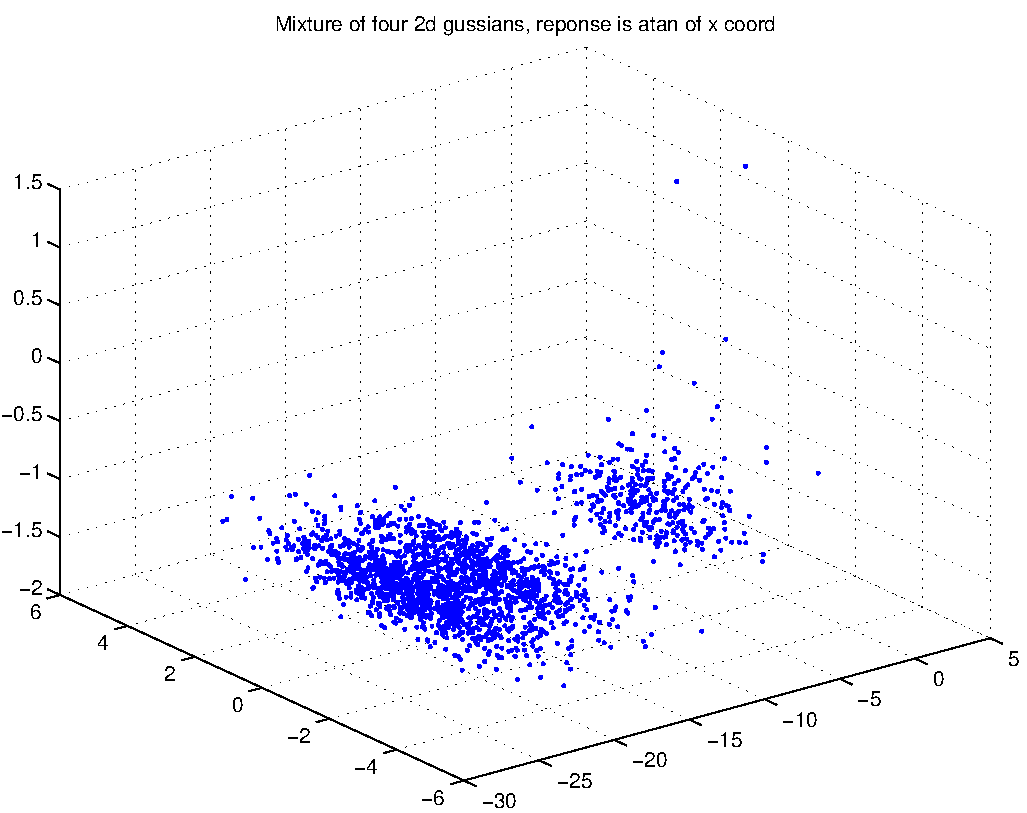
\includegraphics[width=10.0cm,height=10.0cm]{AtanDataSet.pdf}

\subsubsection{3 x 1 Linear Regression}
Sample size = 4000

Number of features = 3

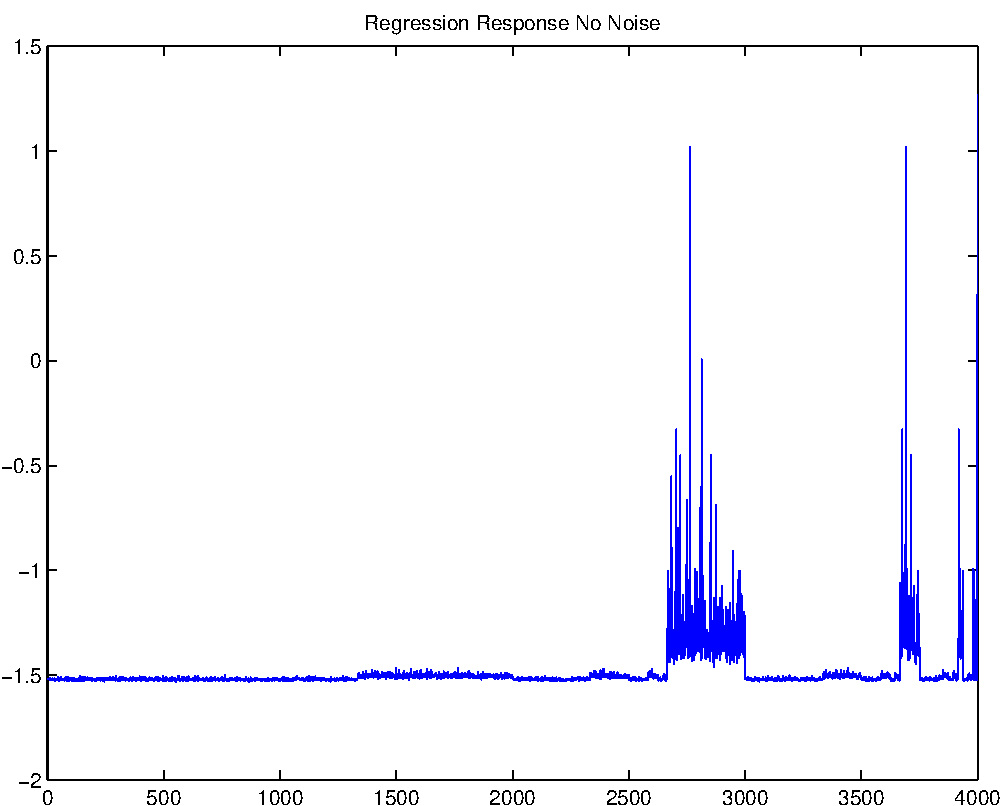
\includegraphics[width=10.0cm,height=10.0cm]{AtanDataSet_regression_response_no_noise.pdf}

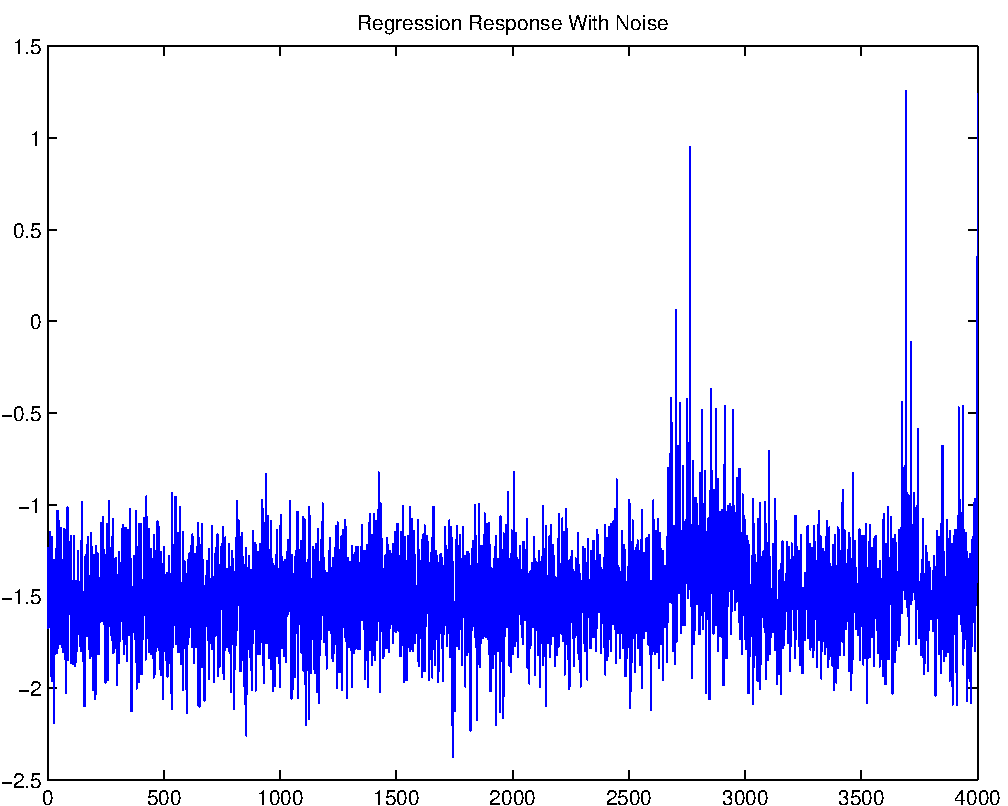
\includegraphics[width=10.0cm,height=10.0cm]{AtanDataSet_regression_response_with_noise.pdf}

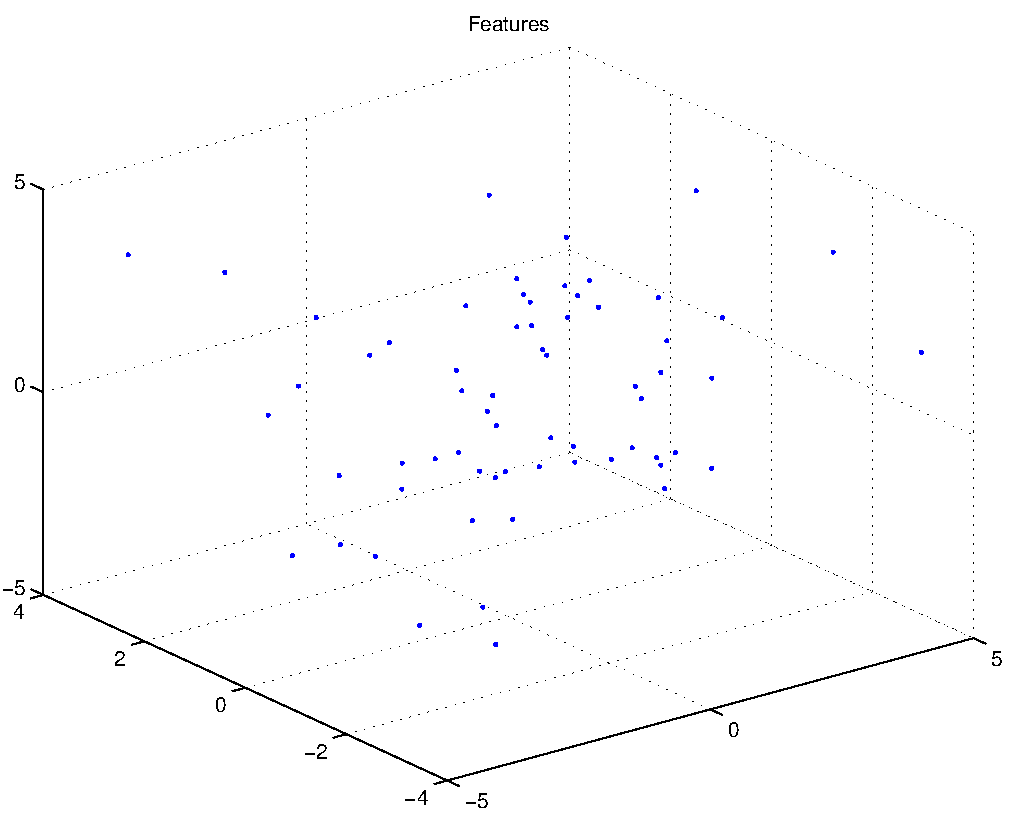
\includegraphics[width=10.0cm,height=10.0cm]{regression_features.pdf}

Response
-1.43591
-1.65403
-1.35841
1.62861
-1.31177
-1.32991
-1.17566
1.58583
-1.32446
-1.1459
-1.60304
0.355108
-1.74172
-1.487
-1.20725
0.929465
-1.17477
-1.36398
-1.77529
1.23309
-1.42294
-1.5148
-0.99204
1.04457
-1.47739
-2.17286
-1.10275
1.45417
-1.45464
-1.75051
-1.29873
1.53846
-1.80555
-1.77319
-1.46602
1.62233
-1.26056
-1.48332
-1.09481
1.07233
-1.17269
-1.37689
-0.928347
1.35367
-1.23084
-1.76028
-1.3358
1.14516
-1.52267
-1.06372
-1.18884
1.58285
-1.55745
-1.74396
-1.23503
1.18468
-1.457
-1.12413
-1.51461
1.13248
-1.48968
-1.75597
-1.28196
1.23406
-1.81473
-1.29265
-1.39913
0.833173
-1.53401
-1.47596
-0.922315
1.75072
-1.73665
-1.20802
-1.27511
1.06809
-1.5995
-1.99582
-0.560041
1.33649
-1.43988
-1.51288
-1.45924
1.81524
-1.34042
-0.985938
-1.16933
1.42019
-1.85039
-1.54254
-1.28675
1.48222
-1.3884
-1.51723
-1.26788
1.17528
-1.37053
-1.19198
0.240696
1.07926
-1.82044
-1.50086
-1.04249
1.0923
-1.69809
-1.8111
-1.12227
1.39849
-1.61492
-1.61637
-1.71357
1.36575
-1.17737
-1.35855
-1.55076
1.24813
-1.81242
-1.40133
-1.655
1.31251
-1.67469
-1.61367
-1.70657
1.04916
-1.80347
-1.54038
-1.50167
1.4005
-1.41139
-1.22453
-1.43446
1.26447
-1.69721
-1.64088
-1.21417
1.38307
-1.58308
-1.76381
-1.60968
1.22656
-1.66463
-1.44175
-1.00929
1.11927
-1.78486
-1.14433
0.00557643
1.97363
-1.63513
-1.76892
-1.75062
1.08996
-1.48388
-1.71093
-1.32797
1.2322
-1.67855
-1.47035
-1.90984
1.14259
-1.38388
-1.28393
-0.990676
1.46334
-1.67988
-1.5701
-0.958005
1.68889
-1.7073
-1.46645
-0.456024
1.4626
-1.37981
-1.18246
-1.09521
0.917664
-1.62223
-1.74401
-0.45417
1.56552
-1.4828
-1.55622
-0.948877
1.34555
-1.48533
-1.81181
-1.02726
1.52015
-1.55457
-1.43179
-1.51223
1.63624
-1.73618
-1.37542
-1.34259
1.33796
-2.01623
-1.40264
-1.43185
1.08337
-1.27002
-1.34612
-1.85704
1.10659
-1.34929
-1.39055
-1.84651
1.43921
-1.46958
-1.21415
-1.43103
1.41034
-1.61809
-1.7289
-1.16641
1.24528
-1.51316
-1.79665
-1.5597
1.30479
-1.8153
-1.41762
-1.41226
1.35529
-1.4504
-1.38207
-1.52432
1.16274
-1.53788
-1.07703
-1.20074
1.48921
-1.39722
-1.16118
-1.48282
1.14267
-1.51142
-1.41583
-1.05937
1.84957
-1.47828
-1.51374
-1.4088
1.24561
-1.33128
-1.73047
-1.16156
1.26051
-1.97217
-1.51077
-1.37693
1.32273
-1.43465
-1.34887
-0.930818
1.27524
-1.32995
-1.55402
-1.05451
0.941748
-1.96307
-1.46394
-0.811841
1.49563
-1.66043
-1.17397
-1.16678
1.62659
-1.56826
-1.61921
-1.33713
1.55341
-1.62274
-1.41428
-1.32739
1.46764
-1.19522
-1.72505
-0.985426
1.03471
-1.34569
-1.4419
-0.858916
1.06758
-1.64345
-1.58642
-1.54969
1.24505
-1.50449
-1.32771
-0.664183
1.15128
-1.44292
-1.29706
-1.44748
1.20614
-1.41894
-1.46488
-1.62402
0.934648
-1.37517
-1.435
-1.30057
1.35019
-1.67545
-1.58843
-0.948338
1.03558
-1.45419
-1.72578
-1.07613
1.43654
-1.62267
-1.27977
0.52303
1.39176
-1.58756
-1.49987
-1.26409
1.6594
-1.50607
-1.50371
-1.53534
1.43947
-1.11667
-1.56631
-1.26299
1.08761
-1.41542
-1.59024
-1.39206
1.43849
-1.4188
-1.55012
-0.974399
1.13364
-1.42524
-1.20148
-1.67416
1.22249
-1.42585
-1.16944
-1.73699
1.38053
-1.13385
-1.60727
-1.41572
1.16213
-1.40998
-1.41922
-1.55229
1.44513
-1.4654
-1.23485
-0.665645
1.81985
-1.6044
-1.47163
-1.35999
1.35558
-2.12088
-1.42181
-1.56593
1.38695
-1.45537
-1.6628
-1.26726
1.23698
-1.61241
-1.66728
-0.991629
1.39513
-1.51606
-1.67784
-1.35301
1.39935
-1.58071
-1.70972
-1.59267
1.8446
-1.84805
-1.3388
-1.19252
1.1405
-1.59652
-1.60699
-1.05156
1.11386
-1.254
-1.3609
-1.29671
0.251363
-1.78072
-1.10058
-1.55209
1.49185
-1.62409
-1.86817
-1.50773
1.15822
-1.10527
-1.5868
-0.994109
1.0078
-1.67862
-1.54145
-1.55926
1.11535
-1.59023
-1.46733
-1.50436
1.46051
-1.48992
-1.4106
-0.350893
1.65765
-1.07635
-1.32318
-1.1786
1.228
-1.49971
-1.81109
-1.24138
1.66558
-0.957246
-1.57253
-0.911891
1.08279
-1.25995
-1.41921
-1.17472
1.68037
-1.16445
-1.34305
-0.414831
1.37331
-1.80706
-1.683
-1.38345
1.29288
-1.56319
-1.57699
-1.39582
1.57811
-1.24874
-1.38217
-1.62792
1.53561
-1.31204
-1.42229
-0.26416
1.62961
-1.81677
-1.5966
0.562467
1.02448
-1.1603
-1.22987
-1.23907
0.978572
-1.9025
-1.54562
-1.79696
0.936588
-1.24685
-1.73442
-1.62481
1.29202
-1.53714
-1.18463
-1.24335
1.1704
-1.08975
-1.15009
-1.3507
1.12579
-1.39842
-1.11126
-1.43641
0.752984
-1.23504
-1.70357
-1.68716
1.51904
-1.73091
-1.52023
-1.33689
0.448949
-1.93043
-1.44818
-1.4677
1.26849
-1.49146
-1.49793
-1.0201
1.46815
-2.0575
-1.3318
-1.66979
1.13433
-1.22752
-1.26858
-1.57933
1.29688
-1.78728
-1.57382
-1.27212
1.17193
-1.84902
-1.39987
-1.38992
1.2991
-1.82426
-1.61205
-1.23007
0.828597
-1.77205
-1.51078
-1.1746
1.43354
-1.27696
-1.78746
-1.30968
1.06331
-1.86383
-1.74484
-1.60516
1.41441
-1.37414
-1.46204
-0.255508
0.922954
-1.4054
-1.48083
-0.80561
1.17716
-2.10989
-1.31315
-1.09269
1.67575
-1.42327
-1.28345
-1.13757
1.24366
-1.48537
-1.41977
-1.1353
1.49692
-1.46879
-0.942888
-1.14598
1.1059
-1.75505
-1.53386
-1.54325
1.11547
-1.61986
-1.37243
-1.17815
1.42363
-1.44639
-1.1243
-0.772213
1.40201
-1.72929
-1.44004
-1.28344
1.24411
-1.0062
-1.5286
-1.25875
1.40623
-1.87435
-1.66206
-1.31636
0.81542
-1.54757
-1.53549
-1.04499
1.29511
-2.00822
-1.3384
-1.04977
0.904481
-1.50465
-1.52321
-1.45226
1.4602
-1.29945
-1.44593
-1.01225
1.132
-1.48308
-1.56705
-1.08076
1.53949
-1.85421
-2.12383
-1.7232
1.29074
-1.71534
-1.49045
-0.412351
1.21727
-1.76516
-1.30184
-1.22268
1.1158
-1.72345
-1.24073
-1.40857
1.21506
-1.40596
-1.41191
-1.3146
1.60389
-1.23422
-1.4992
-1.39663
0.225738
-1.17807
-1.25575
-0.843848
1.71242
-1.52523
-1.33679
-1.22073
1.23932
-1.31068
-1.83485
-1.28334
1.27475
-1.28157
-1.65942
-0.918958
1.6167
-1.46002
-1.75783
-1.21875
1.51235
-1.77178
-1.25203
-0.935508
1.59125
-1.51971
-1.74447
-1.56195
1.7082
-2.0984
-1.25938
-1.35449
1.18761
-1.18807
-2.07767
-0.986003
1.3265
-1.42356
-1.53884
-1.19387
1.33486
-1.43916
-1.69237
-1.20758
0.943011
-1.11186
-1.28694
-1.61905
1.37955
-1.31146
-1.60897
-1.42198
1.21835
-1.43937
-1.73237
-1.61799
1.3381
-1.8211
-1.82515
-1.58743
1.44364
-1.63255
-1.64904
-1.32656
1.50076
-1.46999
-1.41506
-1.24381
1.31527
-1.73967
-1.47037
-1.16806
1.53537
-1.94748
-1.23437
-1.40823
0.910769
-1.43975
-1.72856
-1.65636
0.754631
-1.40224
-1.54891
-1.54125
1.23381
-1.42568
-1.39413
-1.3684
1.59006
-1.77861
-1.38664
-1.24168
1.32883
-1.72371
-1.37988
-1.81208
0.973187
-1.41086
-1.66819
-1.17921
0.95364
-1.49272
-1.28943
-0.963406
1.408
-1.51791
-1.40362
-1.45405
1.09379
-1.28789
-1.53515
-0.963575
0.914001
-1.52994
-1.41451
-1.16032
1.28049
-1.53139
-1.58679
-1.52151
0.959979
-1.33174
-1.73781
-1.38499
1.2992
-1.26702
-1.5495
-1.11806
1.68028
-1.44776
-1.3684
-0.229398
1.39454
-1.43063
-1.89048
-0.940539
1.78349
-1.52937
-1.83309
-1.33256
0.871879
-1.33424
-1.62997
-1.28741
0.97509
-1.17497
-1.61801
-1.17491
1.47172
-1.54411
-1.65141
-1.19899
1.08759
-1.77934
-1.50398
-1.45496
1.1761
-1.74006
-1.41216
-1.53015
1.64644
-1.32982
-1.78721
-1.495
1.16479
-1.81009
-1.49178
-1.36648
1.30719
-2.01625
-1.4447
-0.823907
1.18344
-1.64955
-1.6994
-1.12877
1.00034
-1.53081
-1.28757
-1.37254
0.566754
-1.4136
-1.78415
-1.83948
1.01197
-1.41833
-1.6394
-1.26218
0.796834
-1.1835
-1.18186
-1.12505
1.07003
-1.58913
-1.57116
-0.856137
1.19672
-1.33746
-1.37846
-1.35668
1.51994
-1.0884
-1.50212
-1.40812
1.3093
-1.47248
-1.30761
-1.57018
1.35614
-1.56252
-1.89269
-1.39454
1.27669
-1.18248
-1.46113
-1.37169
1.09333
-1.15638
-1.30226
-1.38559
0.817941
-1.44735
-1.26738
-1.46938
1.18607
-1.99341
-1.32026
-1.41061
0.907181
-2.08839
-1.57251
-1.66423
1.55392
-1.62124
-1.57334
-2.0097
1.14367
-1.80117
-1.41472
-1.19926
1.13812
-1.52996
-1.73451
-1.4793
1.30075
-1.47864
-1.29001
-1.5142
1.55924
-1.65426
-1.80979
-1.31957
1.40263
-1.67101
-1.33564
-1.10224
1.03136
-1.69223
-1.5023
-1.68357
1.17496
-2.00568
-1.13229
-1.33716
1.07045
-1.35085
-1.405
-1.50615
1.05173
-1.65418
-1.31143
-1.39691
1.4088
-1.56145
-1.17686
-1.36691
1.50804
-1.45354
-1.18693
-0.961155
1.64673
-1.80424
-1.61932
-1.0932
1.56606
-1.81181
-1.77649
-1.0248
1.26237
-1.60418
-1.37297
-1.64325
1.17847
-1.29855
-1.20702
-1.70714
1.16798
-1.53528
-1.457
-0.817141
1.22701
-1.39836
-0.96812
-1.50029
1.39021
-1.57804
-1.43444
-0.90566
0.986569
-1.87602
-1.69211
-1.68933
1.10529
-1.75417
-1.58719
-1.14711
1.34243
-1.09767
-1.38914
-1.1992
1.13773
-0.835163
-1.73321
-1.23103
1.37211
-1.55413
-1.52825
-0.714698
1.3024
-1.5179
-1.44636
-1.65916
1.32066
-1.39945
-1.21928
-1.13518
1.57141
-1.82396
-1.65705
-1.0979
1.35452
-1.89535
-1.06932
-1.38137
1.56471
-1.67903
-1.31239
-1.54496
1.54887
-1.67725
-1.36438
-1.35905
1.11703
-1.59428
-1.7133
-1.25468
0.867577
-1.56368
-1.6496
-1.19705
1.26873
-1.27357
-1.42545
-1.18709
1.38456
-1.13835
-1.2502
-1.61616
1.27303
-1.48768
-1.43786
-1.33511
1.13621
-1.35113
-1.38485
-1.73148
1.41057
-1.60673
-1.19529
-1.02312
0.846022
-1.99285
-1.64402
-0.653845
1.17187
-1.6116
-1.59121
-1.08949
1.43239
-1.77527
-1.31546
-1.26518
1.34707
-1.35582
-1.46744
-1.17142
1.4855
-1.81645
-1.43087
-0.921134
1.61937
-1.28886
-1.65798
-0.859524
1.4708
-1.5593
-1.55112
-1.74578
1.3818
-1.53779
-1.43893
-1.11535
1.44543
-1.39446
-1.57145
-0.790327
1.32161
-1.24908
-1.43689
-0.932746
1.60747
-1.50639
-1.4465
-0.89683
1.96084
-1.58657
-1.53067
-1.56494
0.212882
-2.05946
-1.58799
-1.68876
1.43038
-1.45115
-1.99593
-1.61643
1.00356
-1.7136
-1.38346
0.297869
1.39945
-1.38683
-1.40869
-1.41659
0.280137
-1.93296
-1.31123
-1.00668
1.2999
-1.39464
-1.25538
-1.06667
1.69085
-1.70817
-1.38275
-0.941988
0.534518
-1.84401
-1.51935
-1.31064
1.10352
-1.49343
-1.63473
-0.97026
1.40831
-1.60995
-1.62779
-1.35188
1.50742
-1.39472
-1.45517
-1.1074
0.649978
-1.4939
-1.42989
-1.33008
1.54011
-1.27955
-1.3304
-1.26633
1.862
-1.9001
-1.33247
-1.1502
1.02885
-1.07098
-1.75348
-0.58375
0.965155
-1.54227
-1.3222
-2.14773
-0.460791
-1.53783
-1.47883
-1.38067
1.57374
-1.33332
-1.88776
-1.45742
0.863094
-1.54646
-1.27972
-1.44281
0.711296
-1.02428
-1.55529
-0.691838
1.38915
-1.79231
-1.57853
-1.68654
1.25111
-1.48735
-1.85225
-0.840279
1.29503
-1.40893
-1.53976
-1.23369
1.17317
-1.37625
-1.21187
-1.1359
1.35727
-1.65936
-1.2438
-1.32066
0.942127
-1.39116
-1.47366
-1.63402
1.37434
-1.35548
-1.79981
-1.06253
1.15271
-1.64912
-1.29052
-0.969945
0.863071
-1.75864
-1.09908
-1.09082
0.985559
-1.73575
-2.04148
-0.107647
1.634
-1.59833
-1.5494
-1.18993
0.906792
-1.47395
-1.34118
-1.44663
1.39298
-1.17692
-1.5712
-0.827724
1.53456
-1.5976
-1.20809
-0.754198
1.32232
-1.34179
-1.41931
-1.45589
0.961671
-1.53406
-1.26798
-1.08675
1.44202
-1.62465
-1.58139
-1.18833
1.53114
-1.74141
-1.71816
-1.60756
0.790041
-1.36861
-1.46813
-1.53416
1.35609
-1.44151
-1.48945
-0.0285284
1.40291
-1.5187
-1.46618
-1.51629
1.48356
-1.18226
-1.33523
-1.16911
1.46863
-1.61206
-1.33098
-1.30663
1.12127
-1.65836
-1.8159
-1.28494
1.26621
-1.77069
-1.69832
-1.04226
1.02565
-1.28661
-1.37197
-1.5944
1.34955
-1.46096
-1.45085
-1.57662
1.38728
-1.51668
-1.33233
-0.926682
1.152
-1.16643
-1.27173
-0.565118
1.56233
-2.0043
-1.39274
-1.29508
1.75346
-1.53698
-1.44839
-1.17424
1.02571
-1.62817
-1.60066
-1.45622
1.51903
-1.25657
-1.65014
-1.03462
0.973285
-1.66627
-1.14518
-1.14567
1.02971
-2.01256
-1.49533
-1.04036
1.53321
-1.46046
-1.44126
-0.940955
1.24129
-1.66273
-1.63195
-1.23742
1.16223
-1.59606
-1.63735
-1.31225
1.11874
-1.0828
-1.71694
-1.25358
1.70162
-1.33675
-1.71227
-1.59465
-0.142081
-1.4939
-1.33809
-1.55197
1.55431
-1.40251
-1.55403
-1.72428
-0.119481
-1.56472
-1.70302
-1.23256
1.03172
-1.53592
-1.30137
-1.49193
1.26589
-1.61248
-1.62412
-1.5648
1.64028
-1.99428
-1.57653
-0.920159
1.53047
-1.50875
-1.25357
-1.26084
1.58044
-1.4585
-1.79824
-1.22417
1.11435
-1.72576
-1.28011
-1.11003
1.01244
-1.75012
-1.20677
-1.20906
1.19538
-1.68022
-1.6744
-1.42155
1.1169
-1.78416
-1.22947
-1.61241
1.03273
-1.56834
-1.46568
-0.990528
1.52506
-1.66622
-1.52665
-1.34463
1.10669
-1.44421
-1.31611
-1.24031
1.23085
-1.27454
-1.23408
-1.34067
1.68599
-1.64966
-1.38041
-1.3336
1.53281
-1.3966
-1.3064
-1.24595
1.3224
-1.53469
-1.68317
-1.23556
0.89637
-1.97182
-1.24
-1.58372
1.19131
-1.54731
-1.6087
-1.67344
1.3774
-1.54595
-1.22268
-1.15232
1.47953
-2.00163
-1.68209
-1.0623
1.3737
-1.6487
-1.0974
-1.2557
1.5612
-1.56337
-1.34937
-1.70686
1.5338
-1.1912
-1.18282
-1.51212
1.2124
-1.56433
-1.31772
-1.57366
1.55327
-1.35623
-1.63216
-1.06483
0.880496
-1.21909
-1.41972
-1.3699
1.2589
-1.07531
-1.81731
-1.7864
1.34301
-1.68689
-1.36922
-0.664221
1.41914
-1.38209
-1.12324
-1.46999
1.18728
-1.74982
-1.15225
-1.2289
1.33072
-1.3822
-1.46085
-1.17948
1.95249
-1.31215
-1.51806
0.799966
1.42601
-1.73952
-1.22415
-1.82531
1.33562
-1.00418
-1.35348
-1.21957
1.45597
-1.71523
-1.54587
-1.13284
0.853978
-1.3789
-1.84306
-1.09012
1.52601
-1.45791
-1.48279
-1.59665
1.49782
-1.77367
-1.72442
-1.26888
1.06124
-1.28939
-1.59768
-1.28583
1.40832
-1.65272
-1.78973
-1.35567
1.58909
-1.71876
-1.50313
-0.796441
1.10373
-1.48156
-1.43214
-1.42322
1.0691
-1.3461
-1.31605
-1.5323
1.40612
-1.64667
-1.69708
-1.43615
1.493
-1.45966
-1.6381
-1.02202
1.35206
-1.31074
-1.27884
-1.35925
1.39774
-1.77445
-1.42271
-1.19026
1.57761
-1.52681
-1.48813
-1.15267
1.24217
-1.16187
-1.34475
-1.45276
1.15833
-1.29653
-1.54842
-1.43319
1.10541
-1.42963
-1.09398
-1.36907
1.60719
-1.24638
-1.59791
-0.92651
1.29689
-1.69857
-1.25801
-0.969946
1.24973
-1.64569
-1.5406
-1.31171
0.789486
-1.56055
-1.83117
-1.41495
1.26237
-1.16042
-1.36002
-0.980248
1.17821
-1.6573
-1.58488
-1.0948
1.86997
-1.42477
-1.47976
-0.879966
1.48176
-1.96891
-1.34748
-0.810582
1.07096
-1.56659
-1.17626
-1.37128
1.18022
-1.32208
-1.54195
-1.1197
0.930228
-1.37558
-1.59647
-0.941289
1.53947
-1.78723
-1.34805
-1.05612
1.12163
-1.19282
-1.41759
-0.914145
1.46083
-1.81459
-1.00636
-1.5966
1.33539
-1.59693
-1.59381
-1.68218
1.03824
-1.12171
-1.28644
-1.21463
1.62116
-1.42545
-1.47745
-1.58905
1.38965
-1.58558
-1.63339
-1.43947
1.67891
-1.34407
-1.29034
-1.30437
1.21575
-1.75704
-1.68528
-1.20954
1.36585
-1.68148
-1.67744
-1.16375
1.36095
-1.45065
-1.48384
-1.49565
1.42179
-1.8575
-1.08225
-1.19527
1.03248
-1.63038
-1.25536
-1.78515
1.15424
-1.72874
-1.37979
-1.44038
1.24955
-1.33135
-1.54111
-1.40158
1.29241
-1.28321
-1.93476
-1.04288
1.4103
-1.59499
-1.46583
-1.56054
1.08598
-1.18385
-1.47637
-1.34398
1.53745
-1.91973
-1.12044
-1.28768
1.19886
-1.63625
-1.44593
-1.32212
1.38327
-1.59383
-1.49636
-1.09495
0.962613
-1.51563
-1.20072
-1.37207
1.615
-1.36242
-1.333
-0.908005
1.38799
-1.9961
-1.75818
-1.47762
1.06358
-1.46606
-1.65403
-1.67582
0.933833
-1.53135
-1.57854
-0.775384
1.74205
-1.63082
-1.43252
-1.83871
1.12391
-1.80731
-1.605
-1.61187
1.69466
-1.40504
-1.40465
-1.66592
1.27119
-1.69053
-1.87073
-1.04767
1.13927
-1.74765
-1.26104
-1.40798
1.60882
-1.30652
-1.61914
-1.37649
0.970318
-1.49082
-1.61766
0.802411
0.983382
-1.64134
-1.31471
-1.26229
0.960088
-1.75686
-1.48906
-1.34159
1.57468
-1.61194
-1.34571
-1.15286
1.14786
-1.7063
-1.27631
-1.2206
0.8547
-1.71227
-1.75062
-0.903459
0.969868
-1.45979
-1.53195
-1.46882
1.32594
-1.7138
-1.62652
-1.43397
1.30065
-1.13465
-1.3689
-1.34547
1.25027
-1.50573
-1.23985
-1.60237
1.13561
-1.60354
-1.25626
-1.67456
1.34136
-1.29424
-1.34464
-1.15032
1.54998
-1.69932
-1.16623
-0.846868
1.82885
-1.57898
-1.30333
-1.06956
0.957356
-1.70365
-1.66523
-0.90345
1.27389
-1.46038
-1.64078
-1.44834
1.48615
-1.96687
-2.37306
-1.03978
1.4192
-1.80064
-2.00472
-1.52054
1.24591
-1.55614
-1.72321
-1.13147
1.20611
-2.13662
-1.993
-0.665464
1.71496
-1.56844
-1.49502
-1.26796
1.03339
-1.41973
-1.12366
-1.57229
0.769616
-1.72667
-1.74785
-1.46577
1.03784
-1.37725
-1.62631
-1.29184
1.60041
-1.18826
-1.18502
-1.12359
1.49117
-1.66417
-1.57675
-1.14596
1.37463
-1.86255
-1.59286
-1.02988
1.50152
-1.22851
-1.12374
-1.31028
1.3192
-1.54518
-1.45782
-1.52301
1.12411
-1.39275
-1.46101
-1.31682
0.984572
-2.00679
-1.31242
-1.5066
1.26879
-1.69125
-1.49487
-1.48752
0.987649
-1.83508
-1.24969
-1.34183
1.36278
-1.38814
-1.78533
-1.0846
1.32096
-1.44705
-1.63448
-1.18188
1.57105
-1.65254
-1.87278
-2.0112
1.41292
-1.56951
-1.34069
-0.630452
1.69135
-1.36293
-1.67199
-1.26544
1.4624
-1.66525
-1.16905
-0.438915
1.67473
-1.68138
-1.62771
-1.39806
1.21671
-1.71988
-0.99094
-1.31753
1.17618
-1.28765
-1.16873
-1.36044
0.969927
-1.69899
-1.71582
-1.43908
0.610445
-1.35767
-1.32648
-1.65592
1.12485
-1.50342
-1.41325
-1.43769
1.76545
-1.88056
-1.53147
-1.0895
1.37707
-1.90532
-1.74058
-1.19088
1.53501
-1.55764
-1.40014
-1.00183
1.25066
-1.29998
-1.43981
-1.65009
0.991165
-1.37139
-1.24944
-1.17483
1.48361
-1.52066
-1.46001
-1.09591
1.80018
-1.59668
-1.43342
-1.36719
1.6866
-1.54184
-1.36185
-1.56961
1.24099
-1.51089
-1.1103
-1.2276
1.07852
-1.47583
-1.7438
-1.23506
1.16502
-1.11711
-1.81364
-1.39187
1.52156
-1.23769
-1.72553
-1.51249
1.06183
-2.03115
-1.57992
-1.34507
1.39209
-1.63852
-1.3383
-1.23893
0.994306
-1.39518
-1.65207
-1.79761
1.20276
-1.63079
-1.65151
-1.13029
1.6202
-1.36128
-1.69107
-1.22575
1.54103
-1.40221
-1.70557
-1.76579
1.19712
-2.22255
-1.15732
-1.33804
1.38399
-1.72694
-1.3851
-1.23777
1.25617
-1.38799
-1.29913
-1.74385
0.733132
-1.69462
-1.5982
-0.2152
1.43203
-2.14645
-1.45985
-1.1231
1.79799
-1.33354
-1.26003
-1.00017
1.72758
-1.40175
-1.62155
-1.2562
1.34866
-2.18463
-1.83174
-1.50599
1.50597
-1.27018
-1.12271
0.339137
1.33431
-1.25174
-1.71587
-1.51519
1.17674
-1.28964
-1.3214
-1.04635
0.72384
-1.51492
-1.30406
-0.916919
1.38718
-1.68282
-1.37828
-1.12876
1.43919
-0.955194
-1.58959
-0.98188
1.12061
-1.42714
-1.71488
-1.2385
1.16046
-1.50923
-1.40803
-1.21299
0.869166
-1.31483
-1.31019
-0.995872
1.77411
-1.4746
-1.45453
-1.08629
0.939973
-1.29424
-1.80522
-1.63647
1.15853
-0.812536
-1.48778
-0.563454
1.36714
-1.77104
-1.35955
-1.33209
1.17894
-1.15114
-1.32884
-1.28263
1.31372
-1.7343
-1.31431
-0.946174
1.22161
-1.67093
-1.83406
-1.347
0.945994
-1.54644
-1.47339
-1.32711
1.40378
-1.2908
-1.57395
-1.19715
1.65946
-1.57845
-1.41823
-1.07972
1.36361
-1.55827
-1.63987
-1.23229
1.37167
-1.44441
-1.6848
-0.472396
1.25612
-1.75222
-1.27459
-0.954101
1.36923
-1.43438
-1.43745
-1.40285
1.43799
-1.30829
-1.58317
-1.21109
1.3215
-1.45468
-1.60642
-1.50469
1.4776
-1.70495
-1.0687
-1.26848
0.891123
-1.42731
-1.7237
-1.4388
1.08407
-1.50284
-1.36
-1.33356
0.87936
-1.42838
-1.76154
-1.45665
1.52024
-1.53733
-1.34703
-1.50868
1.33689
-1.54936
-1.34029
-1.12807
1.27908
-1.51534
-1.56204
-1.53023
1.3675
-1.40362
-1.41668
-1.04012
1.7286
-1.3074
-1.25818
-1.22682
0.719895
-1.77894
-1.78472
-1.10875
1.40067
-1.36977
-1.58982
-1.17863
1.28894
-1.37374
-1.68785
-1.49253
0.479914
-1.49935
-1.80546
-1.46252
1.65686
-1.62439
-1.65229
-1.04576
1.11712
-2.00162
-1.29444
-1.51281
1.46471
-1.58141
-1.40706
-1.52574
1.34825
-1.282
-1.63452
-1.15279
1.43763
-1.30407
-1.84774
-0.692443
1.42038
-1.32642
-1.45437
-1.20329
1.55953
-1.46055
-1.46935
-0.714458
1.10665
-1.64296
-1.50655
-0.716621
0.819552
-1.69226
-1.41508
-1.40848
1.11046
-1.68151
-1.40523
-1.59907
1.15841
-1.43397
-1.4394
-0.980593
1.42263
-1.40204
-1.47896
-1.01045
1.34489
-1.53444
-1.80477
-1.26817
1.66833
-1.75156
-1.08393
-0.841831
1.20819
-1.6734
-1.35143
-1.04698
1.5243
-1.21883
-1.64772
-1.54773
1.53504
-1.51225
-1.40659
-1.30125
1.45876
-1.86344
-1.5453
-0.341772
1.24483
-1.38368
-1.5195
-0.361843
1.19031
-1.47323
-1.48274
-1.49824
1.14913
-1.80958
-1.64905
-1.17563
1.31358
-1.19048
-1.76614
-1.14085
1.72058
-1.75345
-1.44696
-1.58262
1.2932
-1.41553
-1.37223
-1.05028
1.26108
-1.56595
-1.53975
-1.02663
1.20676
-1.23089
-1.07576
-1.63028
0.511799
-1.49744
-1.72897
-1.46187
1.36783
-1.36338
-1.67094
-0.941403
0.927424
-1.71209
-1.57647
-0.446716
1.49016
-1.42352
-1.00283
-1.47161
1.48995
-1.64285
-1.43603
-0.741485
1.15679
-1.67569
-1.77341
-1.10925
1.21965
-2.00346
-1.65193
-1.10741
1.54186
-1.33402
-1.96129
-1.05588
1.56398
-1.30181
-1.30232
-1.1233
1.30368
-1.52942
-1.4554
-1.09732
1.48672
-1.63082
-1.34207
-1.14999
1.17064
-1.62862
-1.70848
-1.51087
0.95764
-1.46722
-1.72345
-1.36689
1.53639
-1.54299
-1.50887
-0.985668
1.35042
-1.65094
-1.7053
-1.44554
1.42428
-1.49431
-1.38757
-1.26464
1.71079
-1.72399
-1.74564
-1.59974
0.992657
-1.63926
-1.30845
-1.39771
1.24425
-1.90606
-1.36096
-1.51625
1.02535
-2.00094
-1.42225
-1.45233
0.375188
-1.55205
-1.49655
-1.50457
0.748279
-1.44731
-1.52289
-1.20452
1.50571
-1.24251
-1.23209
-1.39988
1.65877
-1.48963
-1.38489
-1.69308
1.37873
-1.33815
-1.74212
-1.35194
1.24968
-1.51788
-1.30459
-1.16264
1.41842
-1.47953
-1.9463
-0.961162
1.32498
-1.51642
-1.36163
-1.22759
1.3868
-1.43295
-1.43865
-1.42891
1.17703
-1.40632
-1.41372
-1.59805
1.06486
-1.49416
-1.24354
-1.00621
1.18459
-1.48371
-1.6868
-1.24754
1.39012
-1.60023
-1.70986
-1.33472
1.61863
-1.31944
-1.72831
-1.28278
1.4614
-1.68076
-1.52075
-0.983626
1.58628
-1.54644
-1.37899
-1.39444
1.24184
-1.68718
-1.13293
-0.69365
1.78727
-1.37658
-1.55547
0.0783144
1.66724
-1.52808
-1.28458
-1.41328
1.47649
-1.49808
-1.52539
-1.15347
1.1748
-1.43494
-1.38113
-1.69719
1.3044
-1.34624
-1.472
-1.0461
1.49485
-1.37236
-1.48131
-1.0072
1.26031
-1.57758
-1.41045
-1.27507
1.3372
-1.79579
-1.53315
-1.4743
0.793941
-1.29736
-1.54394
-1.81324
1.05052
-1.41599
-1.52822
-0.583886
1.59983
-1.6069
-1.45333
-1.07216
0.90283
-1.31723
-1.66488
-1.76793
0.946053
-1.33455
-1.10792
-1.02566
1.62522
-1.35269
-1.74729
-1.29399
0.871379
-1.45135
-1.10963
-1.35937
1.06821
-1.49028
-1.50782
-1.22829
0.802581
-1.46107
-1.65079
-0.982819
1.31447
-1.48418
-1.08197
-1.3262
1.55019
-1.41562
-1.55852
-1.30227
0.843759
-1.49729
-1.6396
-0.914292
0.798709
-1.57694
-1.68177
-1.13909
1.97943
-1.29412
-1.57277
-1.47208
1.46433
-1.70727
-1.58197
-1.26146
1.39054
-1.46138
-1.33256
-1.40183
1.4717
-1.53434
-1.83083
-1.42841
1.25492
-1.71412
-1.65908
-1.12471
1.20231
-1.28921
-1.62117
-0.999836
1.3002
-1.43139
-1.42503
-1.06654
1.33545
-1.57956
-1.23155
-1.4384
1.04238
-1.60398
-1.45597
-1.54944
1.07426
-1.26338
-1.92354
-1.29762
1.36473
-1.55328
-1.84091
-1.41557
1.18814
-1.67431
-1.41407
-1.481
1.33099
-1.7236
-1.53066
-1.07268
1.14795
-0.965893
-1.67745
-1.22716
0.819078
-1.57021
-0.977882
-1.34401
1.32965
-1.70894
-1.67155
-1.67426
1.69864
-1.69694
-1.84033
-1.58601
1.18978
-1.08332
-1.25046
-0.956413
1.2334
-1.7135
-1.69104
-0.705957
1.57585
-1.6237
-1.79082
-1.62911
1.18902
-1.47221
-1.45992
-1.10241
1.29423
-1.4433
-1.65337
-1.5316
1.60125
-1.2996
-1.19321
-1.4912
-0.105221
-1.31811
-1.30542
-1.25294
1.47238
-1.55143
-1.66373
-1.26193
1.18954
-1.24383
-1.85699
-0.877462
1.64307
-1.55565
-1.45306
-1.80941
0.831245
-1.01977
-1.05541
-1.24354
1.4818
-1.61364
-1.55647
-1.20618
1.08884
-1.26802
-1.31979
-1.26594
1.25714
-1.68953
-1.31189
-1.52751
0.851377
-1.30677
-1.26698
-1.50748
1.6507
-1.38673
-1.21647
-1.31483
1.62797
-1.46748
-1.41667
-1.49894
0.980127
-1.66492
-1.44515
-1.16572
1.71181
-1.48955
-1.43486
-1.5304
1.07553
-1.81581
-1.66621
-0.364422
1.51814
-1.65276
-1.84024
-1.10838
1.39682
-1.67888
-1.6506
-1.23593
1.37662
-0.98346
-1.8003
-1.67732
0.946598
-1.10289
-1.77319
-1.14367
1.30112
-1.83195
-1.48552
-1.35663
1.5691
-1.28194
-1.14186
-1.44313
1.35384
-1.82099
-1.66432
-1.21097
1.35395
-1.4691
-1.18308
-0.903207
1.57567
-1.88889
-1.45719
-1.30538
1.39416
-1.25412
-1.69591
-1.5603
1.64867
-1.4925
-1.36315
-1.51458
1.63158
-1.44195
-1.50195
-1.10372
1.07518
-1.24666
-1.92946
-0.971126
1.47846
-1.40154
-1.43476
-1.31153
1.26299
-1.57573
-1.66753
-1.10774
1.43448
-1.45385
-1.31723
-1.37628
1.2584
-1.39048
-1.45659
-1.34154
1.34971
-1.17948
-1.53036
-1.34219
1.541
-1.81487
-1.58714
-1.396
1.47881
-1.60297
-1.58203
-0.989433
1.91439
-1.21952
-1.59723
-1.53055
1.46144
-1.17586
-1.691
-1.26012
1.81179
-1.57573
-1.70167
-1.18848
1.37583
-1.67327
-1.76612
-1.42572
0.916944
-1.4303
-1.95008
-1.11099
1.06634
-1.62691
-1.58819
-1.38499
1.48749
-1.72601
-1.74207
-1.20052
1.75036
-1.60028
-1.8158
-1.19453
1.26486
-1.40216
-1.37459
-1.12809
1.11919
-1.64048
-1.65145
-0.651363
1.77204
-1.14455
-1.06431
-1.36167
1.49868
-1.52292
-1.22033
-1.39399
0.528934
-1.41193
-1.56324
-1.21047
1.30345
-1.53439
-1.5749
-1.69503
1.6466
-1.73603
-1.16381
-1.0576
1.08126
-1.51472
-1.35401
-1.13305
1.36987
-1.44348
-1.35733
-1.78022
1.17345
-1.56541
-1.78189
-1.41998
1.31822
-1.36716
-1.21085
-1.1904
1.50905
-1.46165
-1.61703
-0.977284
1.73898
-0.994345
-1.38118
-1.29757
1.32167
-1.57222
-1.53057
-1.21748
1.09925
-1.55716
-1.37276
-1.48343
1.17103
-1.40468
-1.88927
-1.51955
1.27156
-1.62655
-1.35949
-0.883161
1.27202
-1.5974
-1.27309
-1.65171
1.12135
-1.68567
-1.77247
-1.51056
1.38692
-1.36951
-1.28252
-1.04759
1.49405
-1.69316
-1.44156
-1.18467
1.25727
-1.70777
-1.12131
-1.5292
1.24656
-1.7259
-1.45803
-1.39789
1.12365
-1.47168
-1.73058
-1.33589
0.973135
-1.80304
-1.53207
-1.40823
1.41659
-1.10498
-1.50018
-1.2389
1.41296
-2.01375
-1.34683
-1.39383
1.19629
-1.7682
-1.93596
-1.16102
1.43402
-1.47255
-1.32945
-1.55831
1.103
-1.73699
-0.928318
-1.15569
0.835989
-1.48398
-1.42656
-1.2675
0.396781
-1.83982
-1.54444
-1.61989
1.06893
-1.55866
-1.35678
-1.13168
1.243
-1.2781
-1.63938
-1.39293
1.46289
-1.85722
-1.23108
-2.0776
1.25252
-1.2268
-1.73409
-1.39829
1.46883
-1.68747
-1.43212
-0.843862
1.2209
-1.61115
-1.08461
-1.36687
1.3319
-1.58515
-1.21299
-0.663946
1.05193
-1.3093
-1.22897
-1.6187
1.06403
-1.73324
-1.59489
-1.66571
1.21477
-1.67204
-1.303
-1.42003
0.943868
-1.79153
-1.11799
-0.918818
1.22837
-1.09154
-1.637
-1.81421
1.72375
-1.33362
-1.26119
0.651828
1.7391
-1.35994
-1.83123
-1.61557
0.888466
-1.20504
-1.47626
-1.53438
1.54423
-1.55864
-1.40893
-0.178291
1.48158
-2.00498
-1.33087
-1.00619
1.33363
-1.44885
-1.67485
-2.04346
0.230874
-2.04368
-1.42974
-1.21712
2.15361
-1.60296
-1.14759
-0.706645
1.52793
-1.54753
-1.63342
-1.04028
0.897371
-1.73152
-1.66187
-0.917056
1.40364
-1.19341
-1.54436
-1.48383
1.54207
-1.66711
-1.37025
-1.34949
1.00294
-1.62973
-1.34345
-1.31796
1.30474
-1.48556
-1.65423
-0.943386
1.0637
-1.29912
-1.52008
-1.47368
-0.927151
-1.27455
-1.5538
-1.0354
1.74495
-1.09138
-1.34306
-0.975186
1.40311
-1.71749
-1.48395
-1.43056
1.31046
-1.49648
-1.75385
-0.90225
1.62531
-1.43822
-1.26395
-1.53953
1.33328
-0.933727
-1.56764
-1.36007
1.4053
-1.47384
-1.1433
-0.745171
1.58809
-1.64892
-1.80378
-1.5192
1.54338
-1.97456
-1.6746
-1.16136
1.57515
-1.6237
-1.62903
-0.912948
1.31081
-1.74811
-1.7727
-1.15335
0.899941
-1.86465
-1.08831
-1.56586
1.18389
-1.6149
-1.34807
-1.71342
1.20068
-1.22446
-1.38563
-1.17313
1.4827
-1.45936
-1.72383
-1.42451
1.49997
-1.78656
-1.2733
-0.880883
1.51053
-1.64113
-1.53748
0.164817
1.69802
-1.40095
-1.73028
-1.70258
1.27281
-1.61044
-1.19328
-1.19768
1.41328
-1.5064
-1.81418
-1.55288
1.40454
-1.60927
-1.71434
-1.45023
1.18972
-1.46816
-1.2635
-1.24529
1.60663
-1.93564
-1.62993
-0.782676
0.743586
-1.5691
-1.54775
-0.912981
0.946268
-1.6128
-1.755
-1.11712
1.58804
-1.59473
-1.59058
-1.74714
0.506093
-1.52069
-1.75858
-1.18317
0.807658
-1.55772
-1.56232
-0.879801
0.955431
-1.9601
-1.79197
-1.53514
1.52052
-1.80673
-1.53938
-0.980445
1.87076
-1.99856
-1.39548
-1.60603
1.58006
-1.50581
-1.52549
-1.03138
1.26846
-1.59585
-1.35938
-1.32531
1.58302
-1.27865
-1.54488
-1.09937
1.47248
-1.36123
-1.48134
-1.5219
1.14976
-1.65721
-0.965141
-1.25918
1.18681
-1.96188
-1.18888
-0.905621
1.32226
-1.57352
-1.25276
-1.2061
1.23807
-1.51015
-1.34114
-1.1146
0.814433
-1.7901
-1.50094
-0.421333
1.25131
-1.78339
-1.40046
-1.20282
1.62999
-1.8163
-1.58024
-1.31676
1.15464
-1.52616
-1.53661
-1.38837
1.31554
-1.64738
-1.68237
-1.41454
1.30697
-1.20875
-1.39085
-1.38261
1.44495
-1.56717
-1.34761
-1.34629
1.36477
-1.39447
-0.943852
-1.26713
1.41193
-1.2439
-1.06585
-1.45004
0.867858
-1.51705
-1.50711
-1.3755
1.18162
-1.7415
-1.71544
-1.40683
0.911185
-1.44448
-1.38844
-1.02848
0.981949
-1.54136
-1.56043
-1.59181
0.940249
-1.5253
-2.02377
-1.2038
1.13207
-1.64637
-1.63788
-1.46539
1.18015
-1.20105
-1.40614
-1.61364
1.29093
-1.58525
-1.75802
-1.63431
1.04375
-1.58826
-1.54639
-1.25918
1.26449
-1.68276
-1.42578
-1.27323
1.31494
-1.52541
-1.51449
-1.3421
1.6059
-1.40338
-1.19437
-1.41182
0.98093
-1.2427
-1.70933
-1.11568
1.14088
-1.5835
-1.22004
0.535206
1.55019
-1.90789
-1.8645
-1.29283
1.49615
-1.77211
-1.74824
-1.27393
1.57694
-1.25822
-1.39251
-1.21571
1.16325
-1.32983
-1.42121
-1.15838
1.20763
-1.5016
-1.6022
-1.27467
1.13117
-1.64104
-1.58131
-1.67866
0.977436
-1.05653
-1.44417
-1.48857
1.09138
-1.2507
-1.3362
-1.26739
1.30987
-1.24279
-1.3545
-1.3493
0.934018
-1.41523
-1.22982
-1.5775
1.56057
-1.56189
-1.447
-1.14528
1.52092
-1.8777
-1.65386
-1.07249
0.664133
-1.6531
-1.7531
-1.49294
1.09419
-1.77924
-1.47824
0.332426
1.42454
-1.56497
-1.66772
-0.945646
1.3431
-1.70757
-1.57892
-0.936202
1.19713
-1.66425
-1.34751
-1.21631
1.28482
-1.50173
-1.49679
-1.09135
1.48994
-1.5797
-1.11307
-1.46217
1.31314
-1.47377
-1.10621
-1.29306
1.15226
-1.40684
-1.48104
-1.43599
1.22763
-1.40093
-1.61236
-0.905366
1.27706
-1.78716
-1.72727
-1.51396
1.29903
-1.77348
-1.2678
-1.48411
1.34102
-1.24193
-1.48159
-1.17659
1.19281
-1.8313
-1.35367
-1.33017
1.60146
-1.79421
-1.24462
-1.02962
1.27613
-1.34018
-1.41148
-1.35853
1.18195
-1.43471
-1.29207
-1.40624
1.5213
-1.51523
-1.87334
-1.40867
1.27853
-1.10434
-1.6637
-1.24847
1.73823
-1.04226
-1.15502
-1.54034
0.984578
-1.62329
-1.35608
-1.30395
1.42121
-1.17009
-1.40283
-1.36514
0.875475
-1.78281
-1.50771
-1.11967
1.33223
-1.52618
-1.65928
-1.18368
1.53609
-1.26461
-1.72027
-1.61713
1.16905
-1.53464
-1.74787
-1.14853
1.23192
-1.81748
-1.5706
-0.81717
1.12097
-1.48041
-1.60461
-0.98625
1.04297
-1.70358
-1.50955
-1.48678
1.26485
-1.9019
-1.58817
-1.15134
1.06144
-1.59923
-1.13076
-1.21441
1.29802
-1.49221
-1.3508
-1.66423
1.30397
-1.43979
-1.73341
-1.63966
1.25949
-1.51337
-1.34993
-1.31492
0.963836
-1.53364
-1.76477
-0.179417
1.29373
-1.64706
-1.73525
-1.03648
0.865407
-1.18447
-1.21347
-1.35083
1.2709
-1.70832
-1.77905
-1.39684
1.38253
-1.99091
-1.33944
-1.54505
0.952018
-1.6765
-1.12042
-1.59989
1.15114
-1.89448
-1.13326
-1.12759
1.41558
-1.64181
-1.35032
-1.27096
1.49302
-1.83892
-1.4543
-1.42035
1.5893
-1.56325
-1.46739
-1.20508
1.35383
-1.30726
-1.73124
-0.515102
1.98876
-1.03776
-1.48426
0.149182
1.44549
-1.82694
-1.15467
-1.11205
1.49036
-1.32273
-1.14071
-1.25595
1.39232
-1.70242
-1.52161
-1.24584
1.4333
-1.6259
-1.43314
-1.25332
1.23
-1.4404
-1.26952
-1.45147
1.41353
-1.27045
-1.93196
-1.07868
0.947772
-1.27702
-1.61978
-1.14946
1.4785
-1.53268
-1.30265
-1.20749
0.812478
-1.36264
-1.32058
-1.47128
0.893122
-1.58185
-1.843
-1.15974
1.98078
-1.54263
-1.45065
-1.05519
1.4214
-1.30279
-1.21519
-1.19096
1.70912
-1.42574
-1.44015
-1.3812
1.19647
-1.68908
-1.34316
-1.1038
1.35233
-1.65693
-1.57719
-1.30576
1.17544
-1.71121
-1.54307
-1.22338
1.37242
-1.62075
-1.52301
-1.33264
1.30337
-1.31567
-1.80952
-1.14465
0.92881
-1.38349
-1.42289
-1.24174
1.18267
-1.313
-1.59735
-1.18472
1.54286
-1.1731
-1.64272
-0.887247
1.30868
-1.85868
-1.30253
-0.641807
1.77574
-1.66879
-1.64648
-1.23405
1.09185
-1.45753
-1.36962
-1.37419
1.15889
-1.10756
-1.57508
-1.35387
1.29484
-1.34693
-2.07016
-1.34769
1.14353
-1.44634
-1.4868
-1.37126
1.23961
-1.63829
-1.18917
-1.37699
1.6411
-1.83678
-1.3073
-1.34863
1.19511
-1.32277
-1.65262
-1.29078
1.34305
-1.37587
-1.2175
-1.29521
1.02968
-1.71837
-1.54279
-1.38517
1.44124
-1.4375
-1.86311
-1.04367
1.09131
-1.48971
-1.2323
-1.14814
1.28375
-1.16475
-1.45648
-1.13175
1.72481
-1.43458
-1.66715
-1.36081
1.14734
-1.46988
-1.41064
-1.64598
1.44745
-1.65356
-1.33942
-1.5507
1.24754
-1.62621
-1.56634
-1.71856
1.37158
-1.31532
-1.83564
-1.33785
1.4141
-1.6096
-1.63541
-1.21617
1.47889
-1.86631
-1.42874
-1.39913
1.71141
-1.77789
-1.5939
-1.78087
1.17131
-1.28993
-1.05482
-1.58892
1.17845
-1.59526
-1.2684
-1.15915
0.852
-1.80401
-1.22127
-1.44119
1.38294
-1.39102
-1.62476
-1.34385
1.39441
-1.66981
-1.0646
-0.947034
0.771896
-1.86107
-1.29887
-1.20558
1.30625
-1.44521
-1.53384
-0.954456
1.38277
-1.42955
-1.17212
-1.22694
1.19853
-1.07677
-1.35288
-1.39233
1.346
-1.64093
-2.01386
-1.00224
1.5068
-1.67919
-1.80301
-1.3324
1.07669
-1.64035
-1.59369
-1.62283
1.70169
-1.86449
-1.54817
-1.65618
1.56162
-1.3524
-1.60443
-1.1245
1.31231
-1.75577
-1.68961
-1.16779
1.26894
-1.73447
-1.68579
-1.46686
1.3072
-1.13399
-1.76614
-1.62204
1.07836
-1.32515
-1.44539
-1.89725
0.516011
-1.40505
-1.42572
-0.635878
1.49153
-1.61264
-1.76887
-0.830358
1.29837
-1.68482
-1.67182
-1.63512
0.544817
-1.46321
-1.49748
-1.31605
1.81833
-0.963072
-1.61013
-1.30679
1.44895
-1.24888
-1.97327
-1.07553
1.42383
-1.5478
-1.30699
-1.31837
1.40223
-1.56912
-1.69058
-1.30395
1.09027
-1.64856
-1.78149
-1.10895
1.39432
-2.04328
-1.39194
-1.22117
1.56746
-1.19036
-1.53949
-0.92902
1.15005
-1.17738
-1.11536
-1.28303
1.50157
-1.57661
-1.45021
-1.5188
1.37963
-1.43966
-1.27509
-1.28323
1.29148
-1.38589
-1.42373
-1.027
0.984213
-1.61906
-1.48164
-0.902281
1.21348
-1.51318
-1.23348
-1.29807
0.942252
-1.62963
-1.33833
-1.23149
1.46703
-1.57893
-1.27897
-1.14728
1.63641
-1.63997
-1.86877
-1.4722
1.04583
-1.84514
-1.80742
-1.5526
1.03299
-1.44646
-1.58257
-1.72264
1.09581
-1.37669
-1.61465
-1.22838
1.39385
-1.43372
-1.72317
-1.19518
1.05369
-1.82538
-1.07074
-1.2148
1.25274
-1.68091
-1.91424
-1.73622
1.20355
-1.85795
-1.73806
-1.15784
1.20283
-1.40483
-1.20634
-1.38068
1.44451
-1.26872
-1.53176
-1.262
0.917992
-1.51542
-1.71467
-1.3016
0.789525
-1.43332
-1.30023
-1.15915
1.19926
-1.67498
-1.33498
-1.26771
1.33313
-1.44419
-1.61186
-1.3318
1.22697
-1.58024
-1.4432
-1.20552
1.34772
-1.58413
-1.44641
-1.36818
1.52901
-1.68647
-1.56838
-1.17151
1.61473
-1.62734
-1.5287
-0.840617
1.58588
-1.6529
-1.5403
-1.90097
1.31043
-1.80355
-1.63744
-1.50128
1.6026
-1.41941
-1.51988
-1.02796
1.22473
-1.61544
-1.52751
-1.24121
1.52743
-1.17654
-1.70089
-1.58057
1.0862
-1.57438
-1.63285
-1.30284
1.13898
-1.11287
-1.75439
-1.10209
0.965967
-1.78527
-1.36639
-1.25329
1.52949
-0.683573
-1.39425
-1.04534
1.45474
-1.47359
-1.45507
-1.13151
0.906081
-1.4061
-1.39767
-1.348
1.15682
-1.57192
-1.81884
-1.52082
1.26238
-1.72663
-1.7195
-1.39377
0.926064
-1.10326
-1.19053
-0.75235
1.40933
-1.43819
-1.79986
-1.21719
1.51147
-1.32049
-1.50206
-0.976711
0.93992
-1.14291
-1.53749
-1.55759
1.44741
-1.38039
-1.35328
-1.20319
1.65884
-1.98638
-1.48754
-1.48932
1.6505
-2.10514
-1.41638
-1.61036
1.07245
-1.37845
-1.67802
-1.47668
1.03656
-1.19132
-1.31001
-1.12713
1.24059
-1.13643
-1.40123
-1.50626
1.34936
-1.39266
-1.51802
-1.41191
0.63477
-1.66182
-1.46851
-1.14252
1.27757
-1.32404
-1.18734
-1.37659
1.97629
-1.79749
-1.67025
-1.02014
1.13047
-1.59039
-1.38162
-1.51601
1.21166
-1.57732
-1.49298
-1.46803
1.41782
-1.80146
-1.74542
-1.0429
1.26989
-0.585326
-1.66178
-1.65394
1.30145
-1.64991
-1.12196
-1.64244
1.11355
-1.31109
-1.52075
-1.25112
1.62876
-1.54263
-1.20326
-1.49222
1.11991
-1.78057
-2.05531
-1.15693
1.60829
-1.35955
-1.81295
-1.77906
1.29443
-1.95108
-1.55788
-1.1929
1.3107
-1.32394
-1.88376
-1.14122
0.791129
-1.63793
-1.79971
-1.94597
1.3982
-1.52775
-1.57136
-1.67733
1.12832
-1.70862
-1.19943
-1.32221
1.41629
-1.71979
-1.35347
-1.21453
1.39714
-1.58748
-1.61399
-0.706494
1.93672
-1.66232
-1.79255
-1.30538
1.57063
-1.4248
-1.55531
-1.43763
0.932325
-1.07031
-1.3736
-0.660413
1.38713
Estimate for Beta
4.07731e-005
-0.00141942
0.998019
QueryPerformanceCounter  =  6.11445
\subsubsection{Linear Regression 3x1}
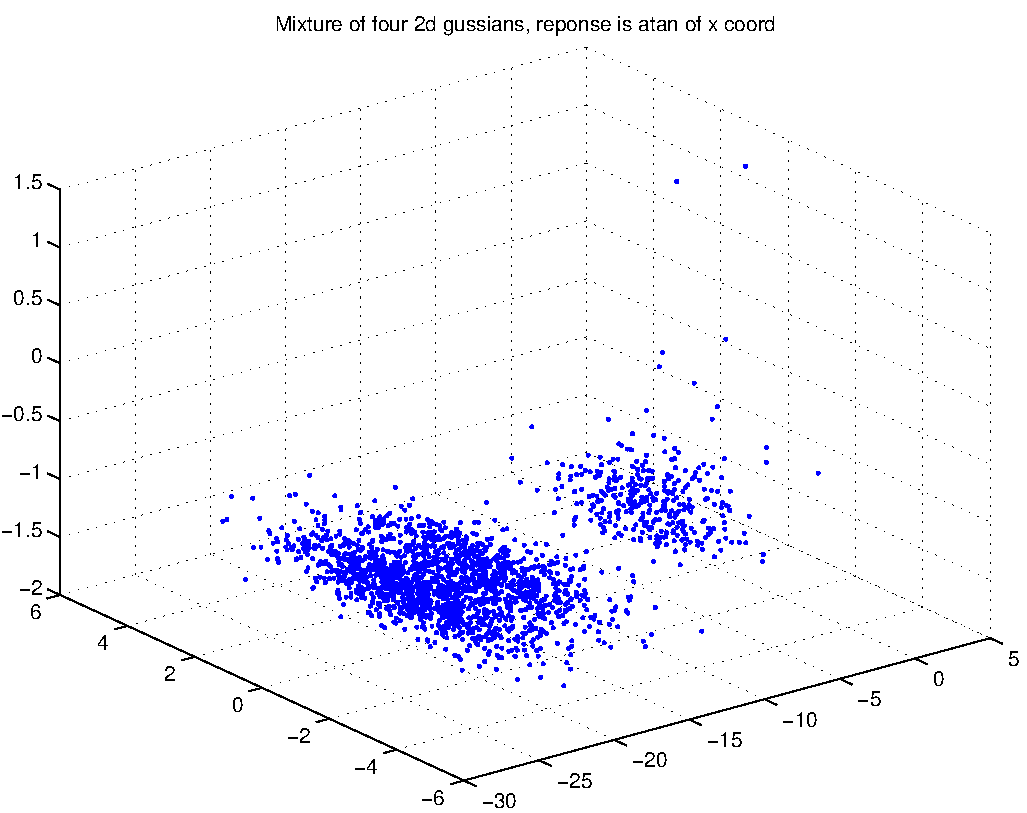
\includegraphics[width=10.0cm,height=10.0cm]{AtanDataSet.pdf}

\subsubsection{3 x 1 Linear Regression}
Sample size = 64

Number of features = 3

$\sigma = \left(
\begin{array}{
ccc}
+3.952 & -0.499 & -0.010 \\
-0.499 & +1.895 & +0.465 \\
-0.010 & +0.465 & +4.477 \\
\end{array}
\right)$ \newline 

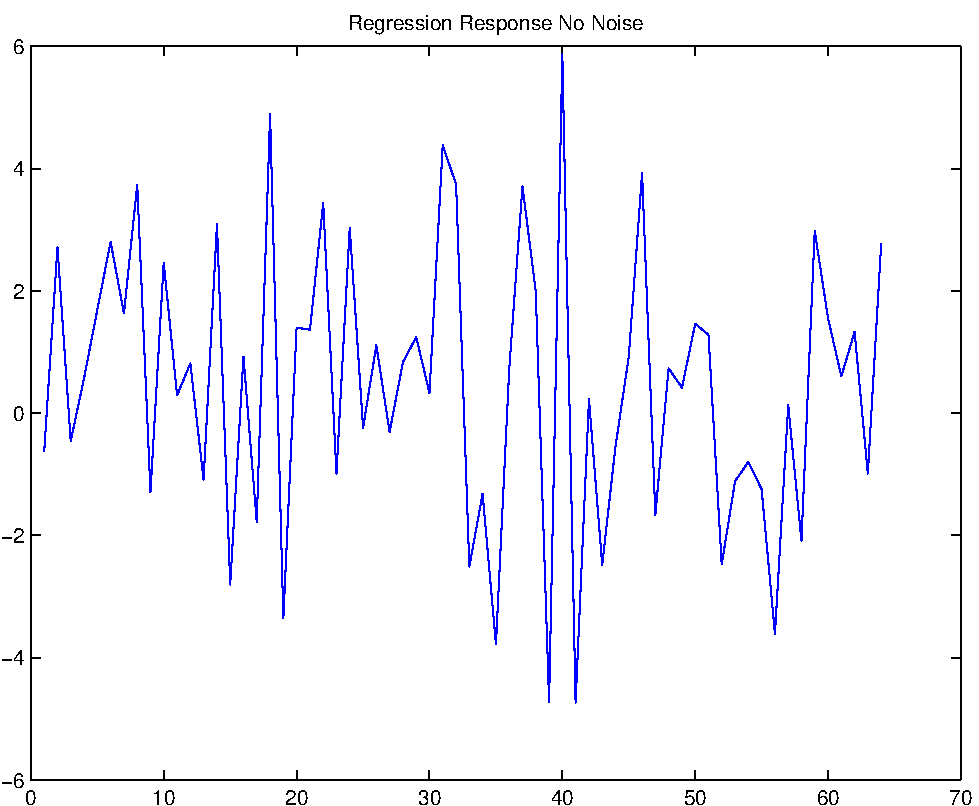
\includegraphics[width=10.0cm,height=10.0cm]{regression_response_no_noise.pdf}

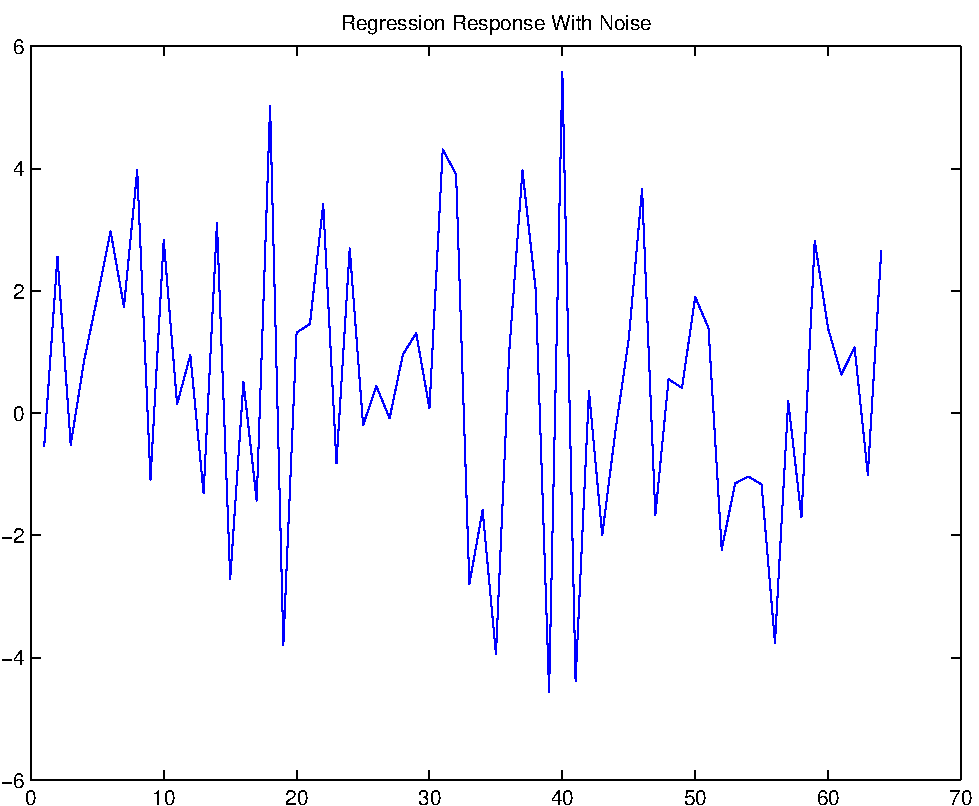
\includegraphics[width=10.0cm,height=10.0cm]{regression_response_with_noise.pdf}

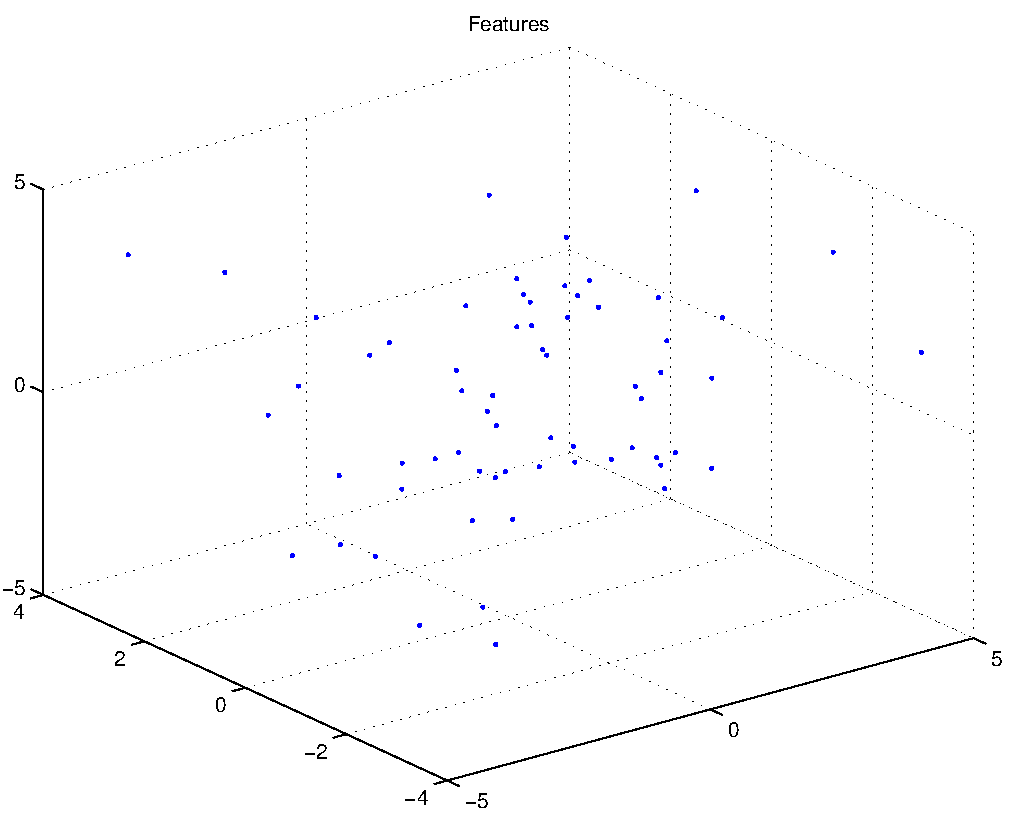
\includegraphics[width=10.0cm,height=10.0cm]{regression_features.pdf}

Beta
+0.817, +0.999, +0.510

Response
+1.137
+3.228
-3.779
+1.819
-5.792
+1.005
-1.506
+3.776
+3.015
+2.559
+0.297
-0.626
-2.981
+1.615
+3.906
+4.129
+0.909
+5.603
-2.563
+3.100
-0.172
-1.010
-0.087
+3.281
+1.523
-1.043
-0.970
-2.123
-4.241
+4.105
+0.366
+2.558
+0.471
+5.304
+0.149
+3.331
+1.370
+2.533
-1.250
+0.575
+2.665
-1.170
-0.659
+0.985
+1.760
-1.782
+1.684
-0.492
-2.543
+1.462
-1.424
-0.499
-0.894
-4.561
-0.578
-0.416
+0.062
+0.278
+2.604
-0.903
+1.477
+1.633
+2.501
+2.923
Estimate for Beta
+0.826
+1.013
+0.491
Error:
+0.008, +0.014, -0.020


QueryPerformanceCounter  =  +4.563
\subsubsection{Fast Gauss Transform}
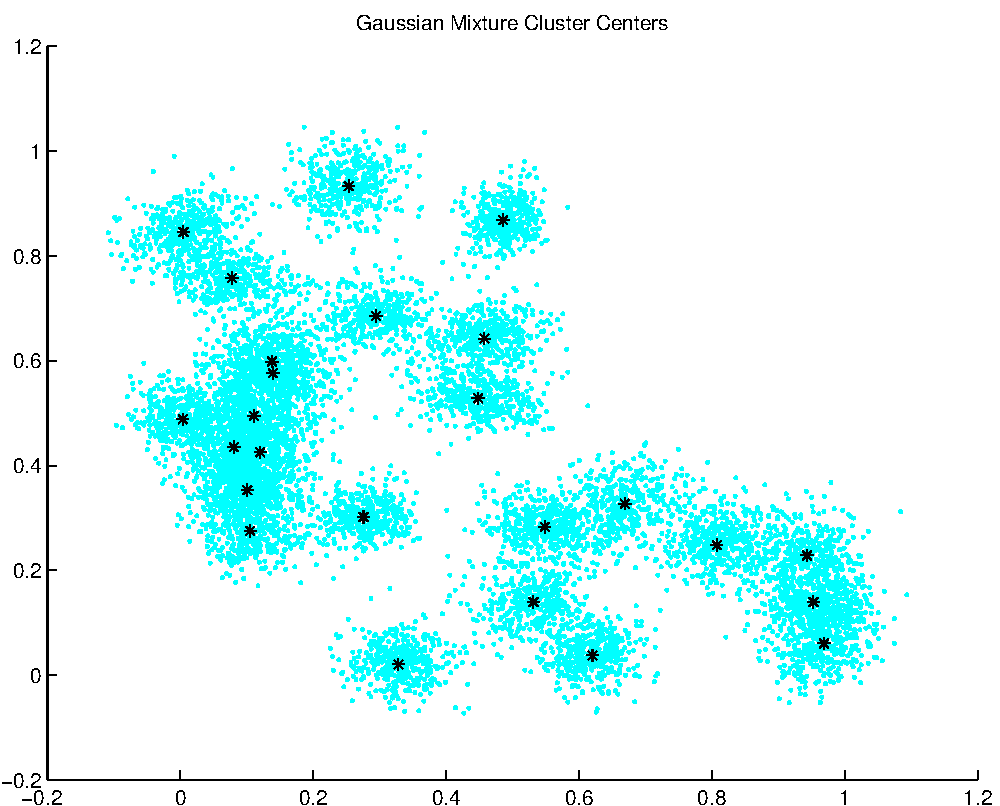
\includegraphics[width=10.0cm,height=10.0cm]{GaussianMixture_ClusterCenters25_Centers.pdf}

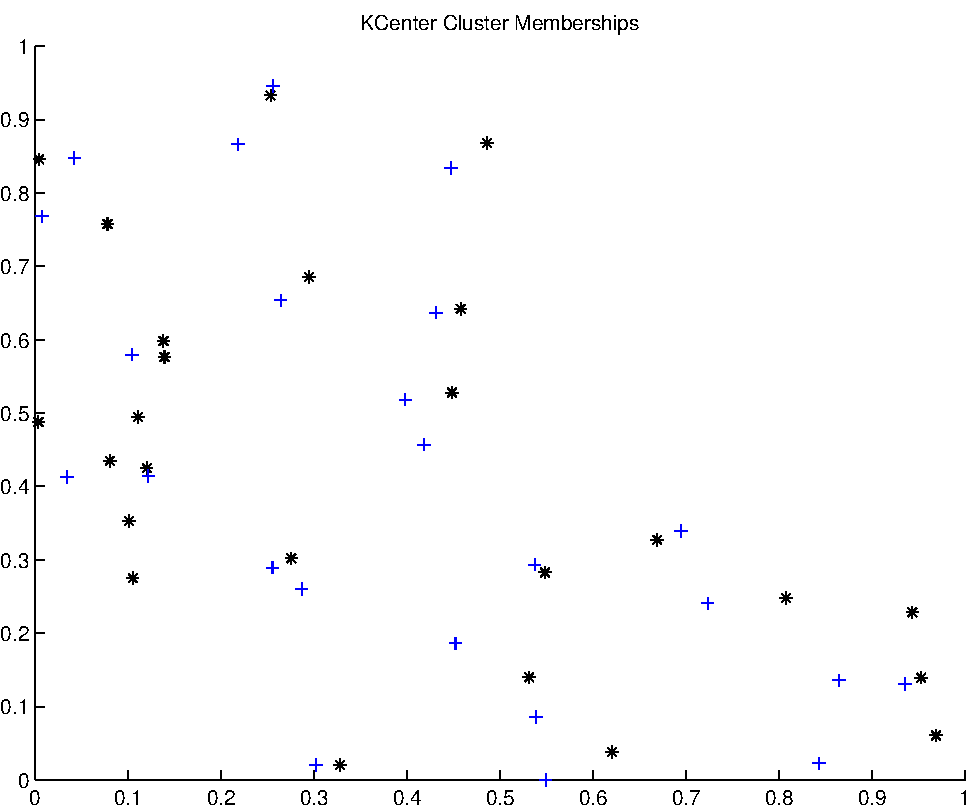
\includegraphics[width=10.0cm,height=10.0cm]{KCenterClusterMemberships_25_Centers.pdf}

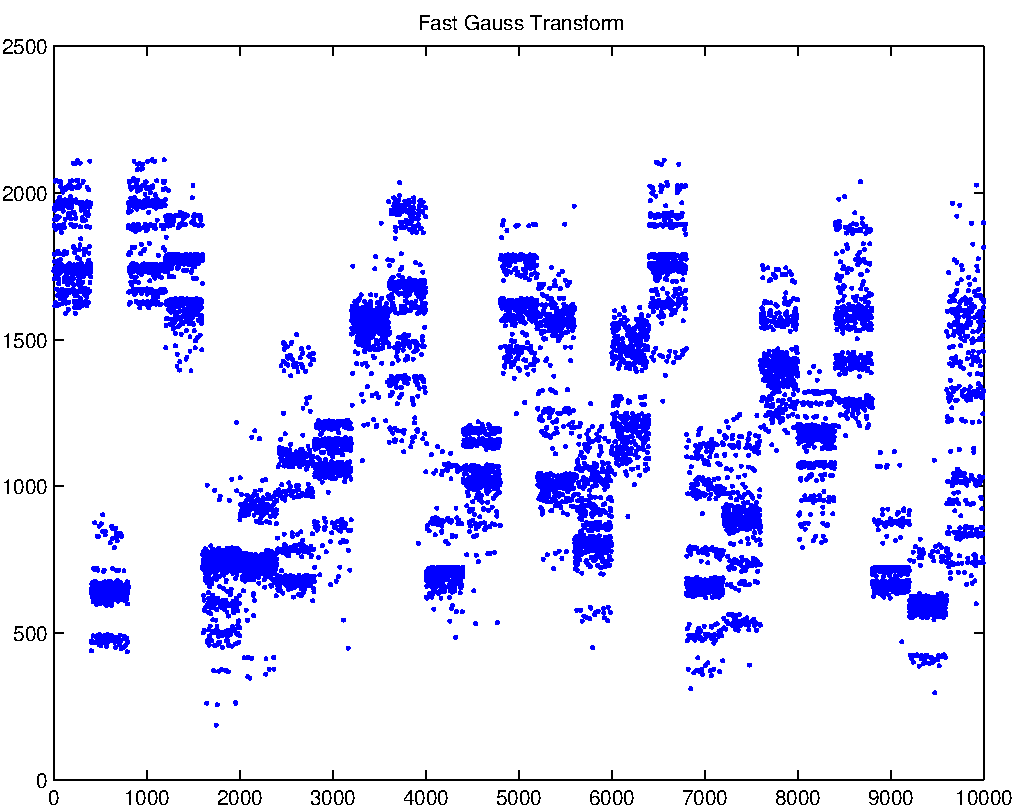
\includegraphics[width=10.0cm,height=10.0cm]{FGT25_Centers.pdf}

QueryPerformanceCounter  =  +7.041
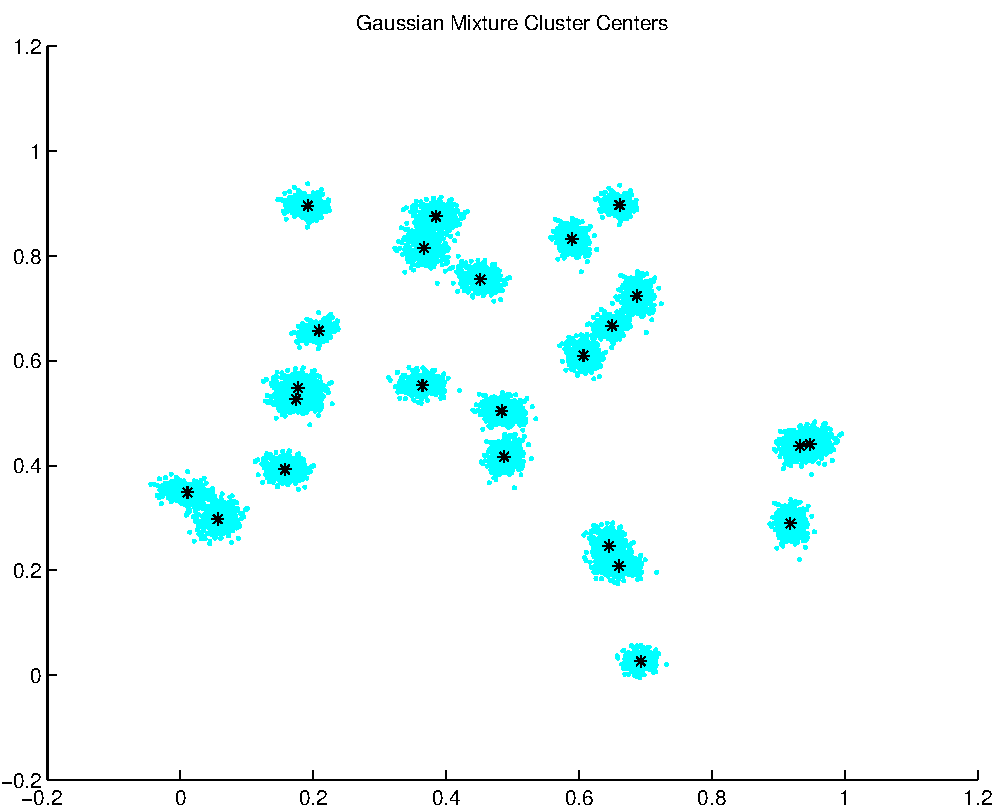
\includegraphics[width=10.0cm,height=10.0cm]{GaussianMixture_ClusterCenters24_Centers.pdf}

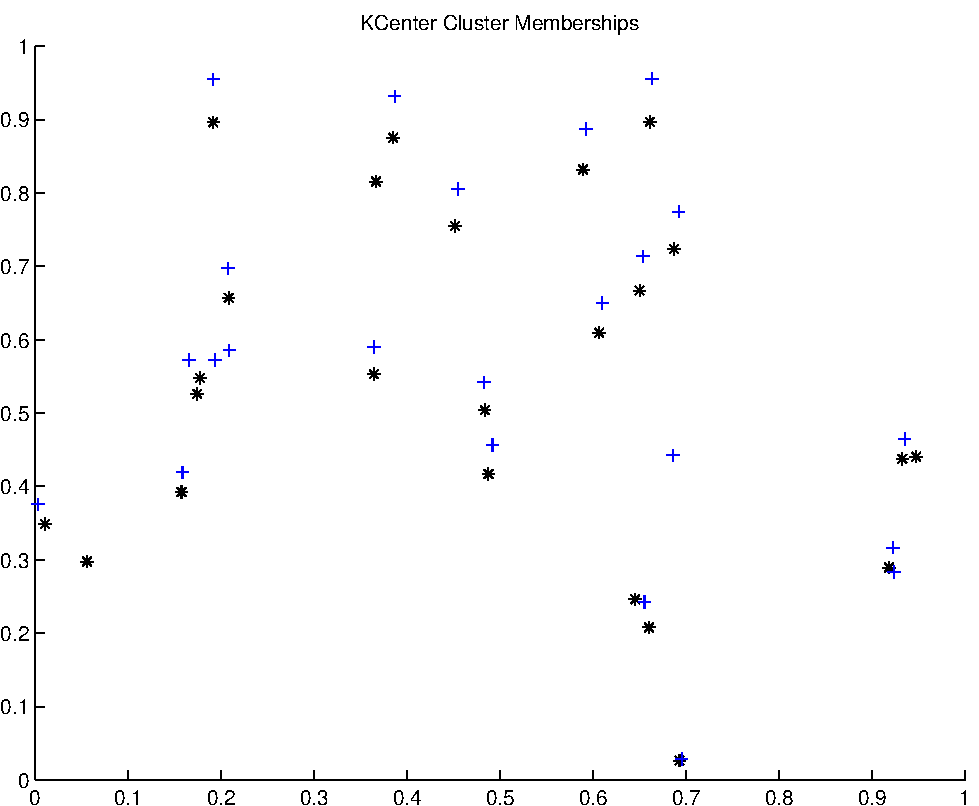
\includegraphics[width=10.0cm,height=10.0cm]{KCenterClusterMemberships_24_Centers.pdf}

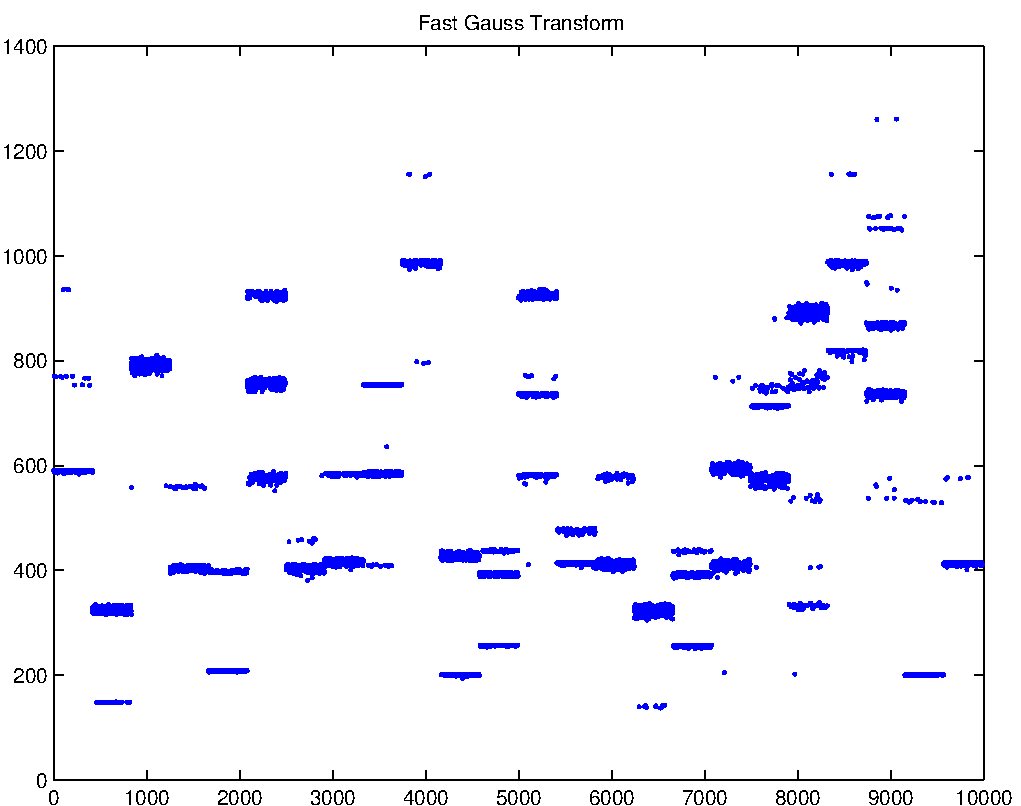
\includegraphics[width=10.0cm,height=10.0cm]{FGT24_Centers.pdf}

QueryPerformanceCounter  =  +7.482
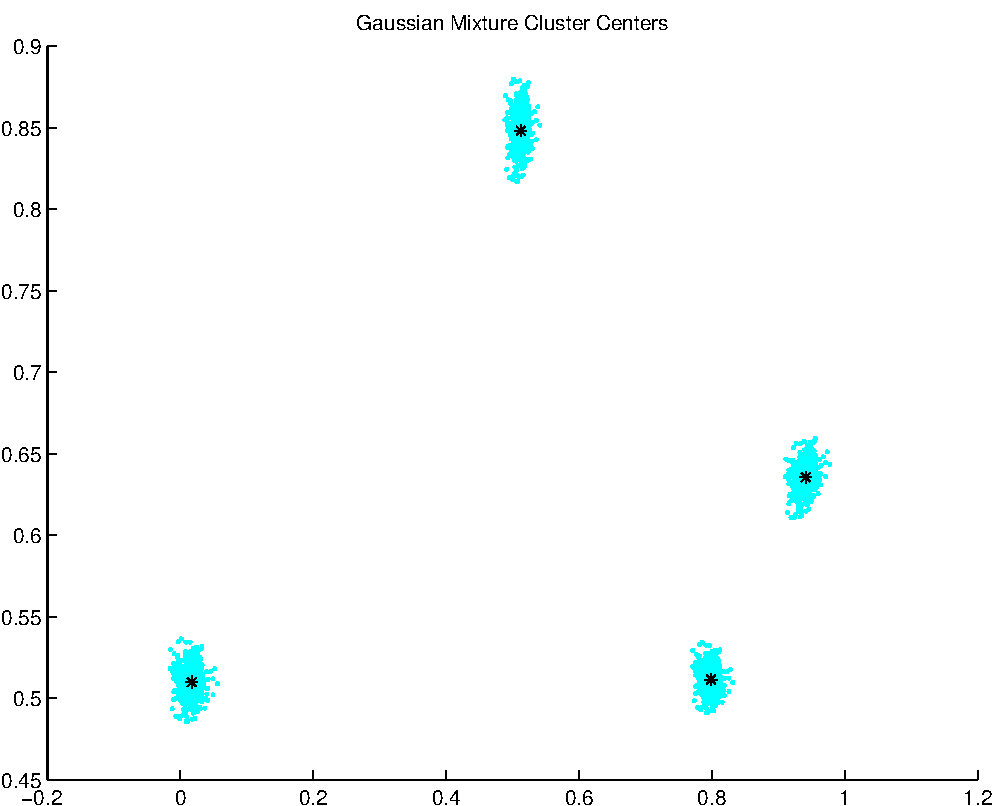
\includegraphics[width=10.0cm,height=10.0cm]{GaussianMixture_ClusterCenters4_Centers.pdf}

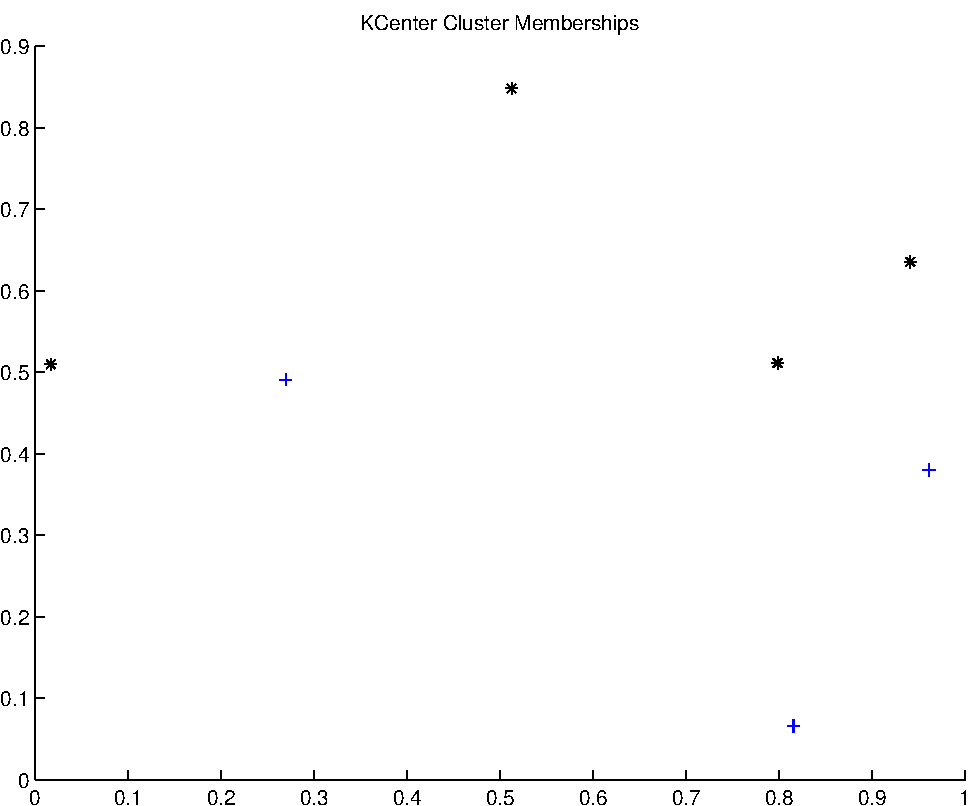
\includegraphics[width=10.0cm,height=10.0cm]{KCenterClusterMemberships_4_Centers.pdf}

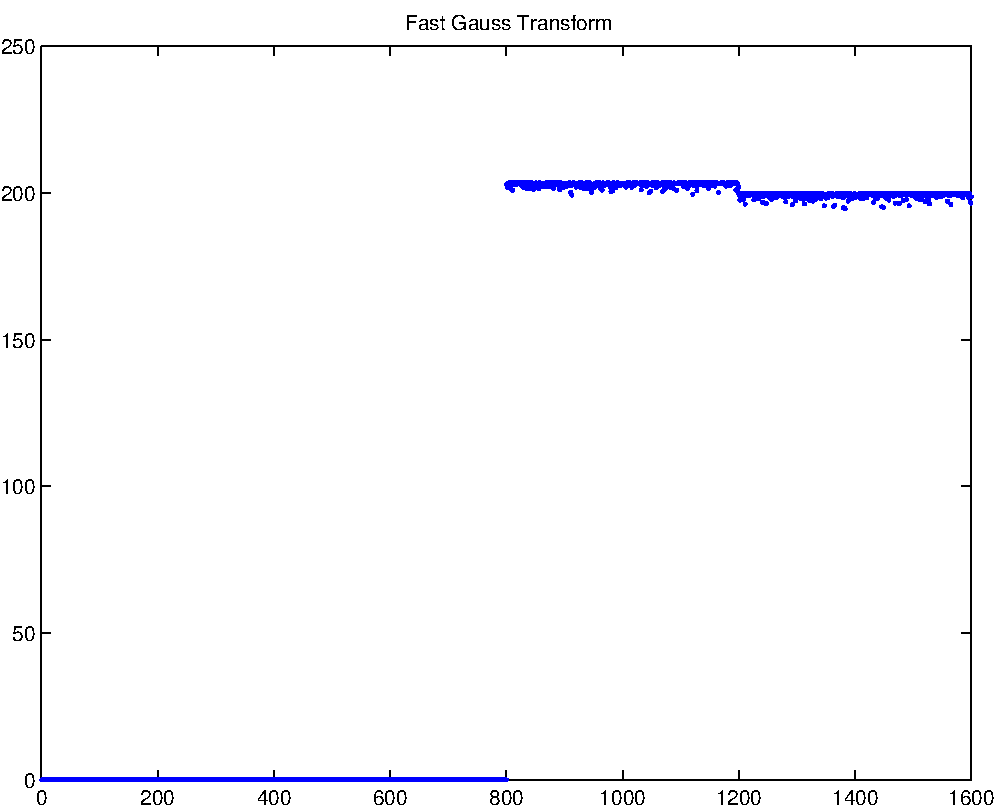
\includegraphics[width=10.0cm,height=10.0cm]{FGT4_Centers.pdf}

QueryPerformanceCounter  =  +3.838
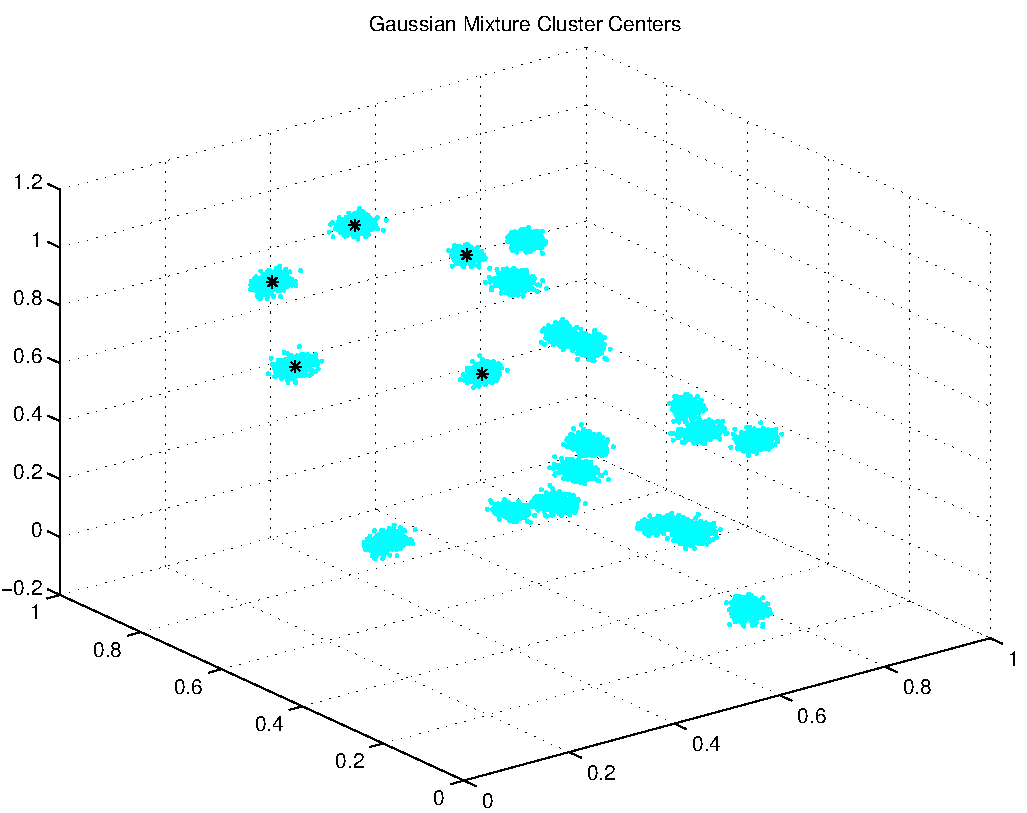
\includegraphics[width=10.0cm,height=10.0cm]{GaussianMixture_ClusterCenters20_Centers.pdf}

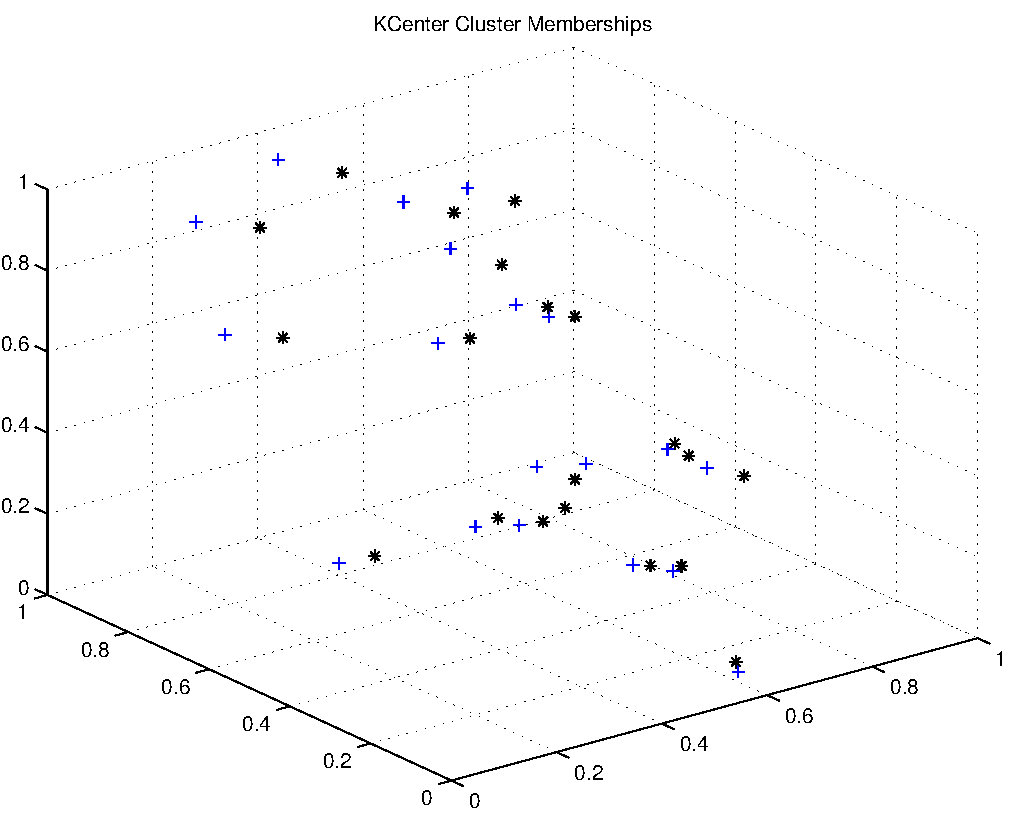
\includegraphics[width=10.0cm,height=10.0cm]{KCenterClusterMemberships_20_Centers.pdf}

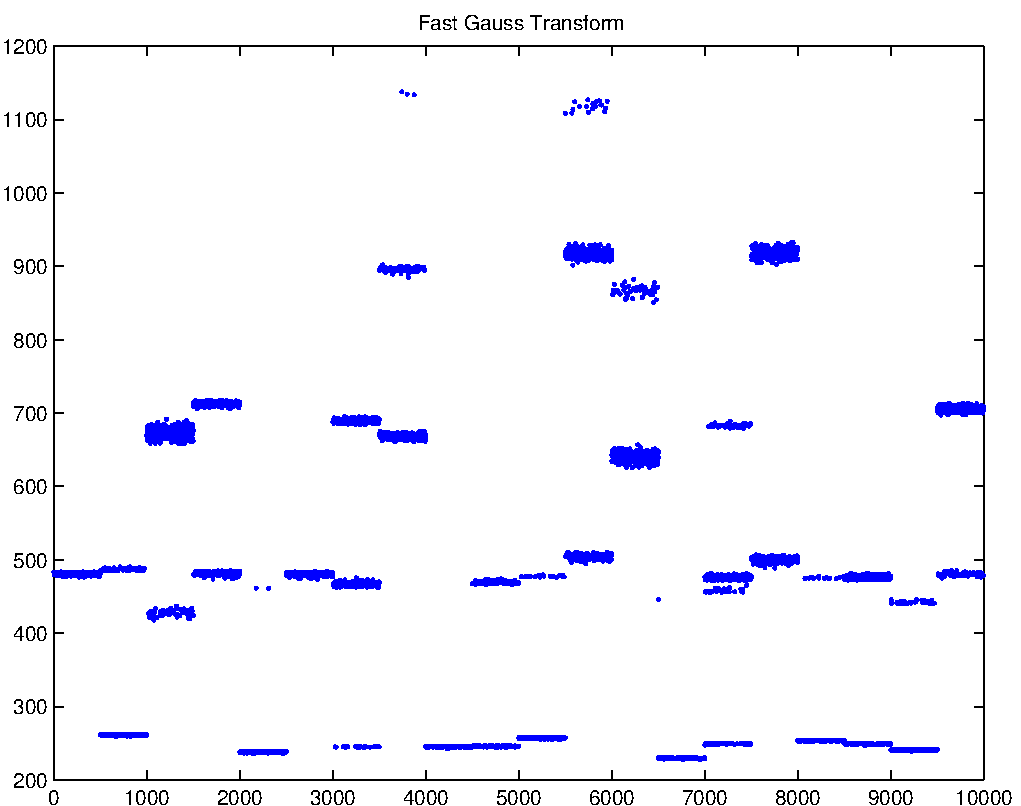
\includegraphics[width=10.0cm,height=10.0cm]{FGT20_Centers.pdf}

QueryPerformanceCounter  =  +6.111
\subsubsection{Matrix Norms}
\subsubsection{Haar Distributed Random Orthogonal Matrix $A \in O(n)$}
 Testing Operator Norm
Number of Dimensions: +12

$A = \left(
\begin{array}{
cccccccccccc}
-0.187 & -0.367 & -0.570 & +0.038 & -0.283 & -0.200 & -0.062 & +0.475 & -0.137 & -0.052 & -0.351 & -0.097 \\
+0.317 & -0.641 & +0.026 & +0.158 & -0.035 & +0.176 & +0.296 & -0.289 & +0.141 & +0.151 & -0.229 & +0.406 \\
+0.018 & +0.221 & -0.633 & -0.135 & +0.202 & +0.328 & -0.036 & -0.111 & -0.040 & +0.563 & +0.169 & +0.151 \\
-0.551 & +0.189 & +0.074 & -0.083 & -0.317 & +0.566 & +0.323 & -0.098 & -0.061 & -0.159 & -0.272 & +0.104 \\
+0.178 & +0.238 & -0.123 & +0.237 & -0.787 & -0.207 & +0.034 & -0.169 & +0.024 & +0.042 & +0.331 & +0.191 \\
-0.215 & +0.231 & -0.359 & +0.436 & +0.334 & -0.304 & +0.129 & -0.327 & +0.242 & -0.370 & -0.151 & +0.190 \\
-0.411 & -0.338 & -0.085 & -0.504 & -0.085 & -0.314 & +0.053 & -0.449 & +0.210 & +0.049 & +0.250 & -0.192 \\
-0.369 & -0.108 & +0.184 & +0.057 & +0.000 & -0.036 & -0.679 & +0.003 & -0.052 & +0.090 & +0.006 & +0.585 \\
-0.287 & +0.107 & +0.267 & +0.276 & -0.015 & -0.244 & +0.218 & +0.220 & +0.389 & +0.643 & -0.171 & -0.099 \\
-0.139 & -0.046 & +0.028 & -0.145 & +0.174 & -0.163 & +0.495 & +0.439 & -0.135 & -0.104 & +0.459 & +0.471 \\
+0.079 & +0.226 & +0.098 & -0.251 & +0.014 & -0.419 & +0.160 & -0.240 & -0.594 & +0.204 & -0.435 & +0.167 \\
+0.265 & +0.262 & -0.048 & -0.534 & -0.090 & -0.066 & -0.058 & +0.182 & +0.573 & -0.132 & -0.313 & +0.285 \\
\end{array}
\right)$ \newline 

$Det(A) :   A \in O(n)$ = (-1.000,+0.000)

$L = \left(
\begin{array}{
cccccccccccc}
+1.000 & +0.000 & +0.000 & +0.000 & +0.000 & +0.000 & +0.000 & +0.000 & +0.000 & +0.000 & +0.000 & +0.000 \\
-0.575 & +1.000 & +0.000 & +0.000 & +0.000 & +0.000 & +0.000 & +0.000 & +0.000 & +0.000 & +0.000 & +0.000 \\
+0.340 & +0.810 & +1.000 & +0.000 & +0.000 & +0.000 & +0.000 & +0.000 & +0.000 & +0.000 & +0.000 & +0.000 \\
+0.746 & +0.899 & +0.310 & +1.000 & +0.000 & +0.000 & +0.000 & +0.000 & +0.000 & +0.000 & +0.000 & +0.000 \\
-0.323 & -0.561 & +0.093 & -0.514 & +1.000 & +0.000 & +0.000 & +0.000 & +0.000 & +0.000 & +0.000 & +0.000 \\
-0.481 & -0.663 & -0.050 & +0.942 & +0.856 & +1.000 & +0.000 & +0.000 & +0.000 & +0.000 & +0.000 & +0.000 \\
+0.669 & +0.439 & -0.160 & -0.114 & -0.417 & -0.617 & +1.000 & +0.000 & +0.000 & +0.000 & +0.000 & +0.000 \\
-0.032 & -0.427 & +0.924 & +0.130 & -0.064 & +0.933 & -0.261 & +1.000 & +0.000 & +0.000 & +0.000 & +0.000 \\
+0.391 & -0.295 & +0.564 & -0.964 & -0.873 & -0.637 & -0.805 & +0.486 & +1.000 & +0.000 & +0.000 & +0.000 \\
+0.521 & -0.016 & -0.352 & -0.588 & -0.421 & -0.945 & -0.351 & -0.643 & +0.784 & +1.000 & +0.000 & +0.000 \\
-0.144 & -0.475 & -0.217 & +0.404 & +0.329 & +0.104 & -0.457 & -0.155 & -0.659 & -0.125 & +1.000 & +0.000 \\
+0.252 & +0.176 & +0.005 & +0.268 & -0.239 & -0.115 & -0.746 & -0.595 & -0.004 & +0.254 & -0.355 & +1.000 \\
\end{array}
\right)$ \newline 

$U = \left(
\begin{array}{
cccccccccccc}
-0.551 & +0.189 & +0.074 & -0.083 & -0.317 & +0.566 & +0.323 & -0.098 & -0.061 & -0.159 & -0.272 & +0.104 \\
+0.000 & -0.533 & +0.069 & +0.110 & -0.217 & +0.502 & +0.482 & -0.345 & +0.106 & +0.059 & -0.385 & +0.466 \\
+0.000 & +0.000 & -0.651 & -0.023 & +0.001 & -0.799 & -0.562 & +0.788 & -0.202 & -0.046 & +0.053 & -0.510 \\
+0.000 & +0.000 & +0.000 & -0.533 & +0.347 & -0.940 & -0.446 & -0.310 & +0.223 & +0.129 & +0.782 & -0.531 \\
+0.000 & +0.000 & +0.000 & +0.000 & -0.833 & -0.150 & +0.231 & -0.627 & +0.197 & +0.095 & +0.424 & +0.262 \\
+0.000 & +0.000 & +0.000 & +0.000 & +0.000 & +1.512 & +0.611 & +0.774 & +0.226 & -0.374 & -1.796 & +0.894 \\
+0.000 & +0.000 & +0.000 & +0.000 & +0.000 & +0.000 & -0.774 & +0.527 & +0.157 & -0.013 & -0.476 & +0.829 \\
+0.000 & +0.000 & +0.000 & +0.000 & +0.000 & +0.000 & +0.000 & -1.573 & +0.004 & +0.960 & +1.424 & +0.292 \\
+0.000 & +0.000 & +0.000 & +0.000 & +0.000 & +0.000 & +0.000 & +0.000 & +1.066 & -0.773 & -1.282 & +1.386 \\
+0.000 & +0.000 & +0.000 & +0.000 & +0.000 & +0.000 & +0.000 & +0.000 & +0.000 & +1.692 & +0.680 & -0.290 \\
+0.000 & +0.000 & +0.000 & +0.000 & +0.000 & +0.000 & +0.000 & +0.000 & +0.000 & +0.000 & -1.671 & +1.630 \\
+0.000 & +0.000 & +0.000 & +0.000 & +0.000 & +0.000 & +0.000 & +0.000 & +0.000 & +0.000 & +0.000 & +2.124 \\
\end{array}
\right)$ \newline 

$L * U  = \left(
\begin{array}{
cccccccccccc}
-0.551 & +0.189 & +0.074 & -0.083 & -0.317 & +0.566 & +0.323 & -0.098 & -0.061 & -0.159 & -0.272 & +0.104 \\
+0.317 & -0.641 & +0.026 & +0.158 & -0.035 & +0.176 & +0.296 & -0.289 & +0.141 & +0.151 & -0.229 & +0.406 \\
-0.187 & -0.367 & -0.570 & +0.038 & -0.283 & -0.200 & -0.062 & +0.475 & -0.137 & -0.052 & -0.351 & -0.097 \\
-0.411 & -0.338 & -0.085 & -0.504 & -0.085 & -0.314 & +0.053 & -0.449 & +0.210 & +0.049 & +0.250 & -0.192 \\
+0.178 & +0.238 & -0.123 & +0.237 & -0.787 & -0.207 & +0.034 & -0.169 & +0.024 & +0.042 & +0.331 & +0.191 \\
+0.265 & +0.262 & -0.048 & -0.534 & -0.090 & -0.066 & -0.058 & +0.182 & +0.573 & -0.132 & -0.313 & +0.285 \\
-0.369 & -0.108 & +0.184 & +0.057 & +0.000 & -0.036 & -0.679 & +0.003 & -0.052 & +0.090 & +0.006 & +0.585 \\
+0.018 & +0.221 & -0.633 & -0.135 & +0.202 & +0.328 & -0.036 & -0.111 & -0.040 & +0.563 & +0.169 & +0.151 \\
-0.215 & +0.231 & -0.359 & +0.436 & +0.334 & -0.304 & +0.129 & -0.327 & +0.242 & -0.370 & -0.151 & +0.190 \\
-0.287 & +0.107 & +0.267 & +0.276 & -0.015 & -0.244 & +0.218 & +0.220 & +0.389 & +0.643 & -0.171 & -0.099 \\
+0.079 & +0.226 & +0.098 & -0.251 & +0.014 & -0.419 & +0.160 & -0.240 & -0.594 & +0.204 & -0.435 & +0.167 \\
-0.139 & -0.046 & +0.028 & -0.145 & +0.174 & -0.163 & +0.495 & +0.439 & -0.135 & -0.104 & +0.459 & +0.471 \\
\end{array}
\right)$ \newline 

$Det(L) :    = (+1.000,+0.000)     Det(U) :    = (+1.000,+0.000)     Det(LU) :    = (+1.000,-0.000)$

$||A||_{L_1}$  = +3.137

$||A||_{L_{\infty}}$ = +3.287

$||A^{-1}||_{L_1}$  = +3.287

$||A^{-1}||_{L_{\infty}}$ = +3.137

$||A||_{L_{\infty}} * ||A^{-1}||_{L_{\infty}} = +10.310$

$||A||_{L_1} * ||A^{-1}||_{L_1} = +10.310$

Frobenious Norm  $||A||_{\textit{F}}$ via $\sum\limits_{i,j =0}^{n} \|A_{i,j}|$   of  $A \in O(n)$  +3.464

$L_1$ condition number of Haar Distributed Random Orthogonal Matrix $A \in O(n)$ +9.220

$A = \left(
\begin{array}{
cccccccccccc}
-0.187 & -0.367 & -0.570 & +0.038 & -0.283 & -0.200 & -0.062 & +0.475 & -0.137 & -0.052 & -0.351 & -0.097 \\
+0.317 & -0.641 & +0.026 & +0.158 & -0.035 & +0.176 & +0.296 & -0.289 & +0.141 & +0.151 & -0.229 & +0.406 \\
+0.018 & +0.221 & -0.633 & -0.135 & +0.202 & +0.328 & -0.036 & -0.111 & -0.040 & +0.563 & +0.169 & +0.151 \\
-0.551 & +0.189 & +0.074 & -0.083 & -0.317 & +0.566 & +0.323 & -0.098 & -0.061 & -0.159 & -0.272 & +0.104 \\
+0.178 & +0.238 & -0.123 & +0.237 & -0.787 & -0.207 & +0.034 & -0.169 & +0.024 & +0.042 & +0.331 & +0.191 \\
-0.215 & +0.231 & -0.359 & +0.436 & +0.334 & -0.304 & +0.129 & -0.327 & +0.242 & -0.370 & -0.151 & +0.190 \\
-0.411 & -0.338 & -0.085 & -0.504 & -0.085 & -0.314 & +0.053 & -0.449 & +0.210 & +0.049 & +0.250 & -0.192 \\
-0.369 & -0.108 & +0.184 & +0.057 & +0.000 & -0.036 & -0.679 & +0.003 & -0.052 & +0.090 & +0.006 & +0.585 \\
-0.287 & +0.107 & +0.267 & +0.276 & -0.015 & -0.244 & +0.218 & +0.220 & +0.389 & +0.643 & -0.171 & -0.099 \\
-0.139 & -0.046 & +0.028 & -0.145 & +0.174 & -0.163 & +0.495 & +0.439 & -0.135 & -0.104 & +0.459 & +0.471 \\
+0.079 & +0.226 & +0.098 & -0.251 & +0.014 & -0.419 & +0.160 & -0.240 & -0.594 & +0.204 & -0.435 & +0.167 \\
+0.265 & +0.262 & -0.048 & -0.534 & -0.090 & -0.066 & -0.058 & +0.182 & +0.573 & -0.132 & -0.313 & +0.285 \\
\end{array}
\right)$ \newline 

$L_{\infty}$ condition number of Haar Distributed Random Orthogonal Matrix $A \in O(n)$ +9.911

Eigenvalues of $A \in O(n)$

(+0.125,+0.992), (+0.125,-0.992), (-0.448,+0.894), (-0.448,-0.894), (-0.764,+0.646), (-0.764,-0.646), (-0.995,+0.100), (-0.995,-0.100), (-1.000,+0.000), (+0.860,+0.510), (+0.860,-0.510), (+1.000,+0.000)

 $|\lambda | : \lambda \in \sigma(A) , A \in O(n)$

+1.000, +1.000, +1.000, +1.000, +1.000, +1.000, +1.000, +1.000, +1.000, +1.000, +1.000, +1.000


Calculating $A^{\dag} A,$  we expect $A^{\dag} A \approx I$

$A^{\dag} A = \left(
\begin{array}{
cccccccccccc}
+1.000 & +0.000 & +0.000 & -0.000 & +0.000 & +0.000 & +0.000 & -0.000 & +0.000 & -0.000 & +0.000 & +0.000 \\
+0.000 & +1.000 & -0.000 & -0.000 & +0.000 & +0.000 & -0.000 & +0.000 & -0.000 & +0.000 & +0.000 & +0.000 \\
+0.000 & -0.000 & +1.000 & +0.000 & +0.000 & -0.000 & -0.000 & -0.000 & +0.000 & +0.000 & +0.000 & +0.000 \\
-0.000 & -0.000 & +0.000 & +1.000 & -0.000 & +0.000 & +0.000 & +0.000 & -0.000 & +0.000 & -0.000 & +0.000 \\
+0.000 & +0.000 & +0.000 & -0.000 & +1.000 & -0.000 & +0.000 & -0.000 & +0.000 & -0.000 & +0.000 & +0.000 \\
+0.000 & +0.000 & -0.000 & +0.000 & -0.000 & +1.000 & -0.000 & -0.000 & +0.000 & -0.000 & +0.000 & -0.000 \\
+0.000 & -0.000 & -0.000 & +0.000 & +0.000 & -0.000 & +1.000 & +0.000 & +0.000 & +0.000 & +0.000 & -0.000 \\
-0.000 & +0.000 & -0.000 & +0.000 & -0.000 & -0.000 & +0.000 & +1.000 & -0.000 & -0.000 & -0.000 & -0.000 \\
+0.000 & -0.000 & +0.000 & -0.000 & +0.000 & +0.000 & +0.000 & -0.000 & +1.000 & -0.000 & +0.000 & -0.000 \\
-0.000 & +0.000 & +0.000 & +0.000 & -0.000 & -0.000 & +0.000 & -0.000 & -0.000 & +1.000 & -0.000 & +0.000 \\
+0.000 & +0.000 & +0.000 & -0.000 & +0.000 & +0.000 & +0.000 & -0.000 & +0.000 & -0.000 & +1.000 & -0.000 \\
+0.000 & +0.000 & +0.000 & +0.000 & +0.000 & -0.000 & -0.000 & -0.000 & -0.000 & +0.000 & -0.000 & +1.000 \\
\end{array}
\right)$ \newline 

Calculating $A^{-1} ,  A \in O(n)$.

$A^{-1} = \left(
\begin{array}{
cccccccccccc}
-0.187 & +0.317 & +0.018 & -0.551 & +0.178 & -0.215 & -0.411 & -0.369 & -0.287 & -0.139 & +0.079 & +0.265 \\
-0.367 & -0.641 & +0.221 & +0.189 & +0.238 & +0.231 & -0.338 & -0.108 & +0.107 & -0.046 & +0.226 & +0.262 \\
-0.570 & +0.026 & -0.633 & +0.074 & -0.123 & -0.359 & -0.085 & +0.184 & +0.267 & +0.028 & +0.098 & -0.048 \\
+0.038 & +0.158 & -0.135 & -0.083 & +0.237 & +0.436 & -0.504 & +0.057 & +0.276 & -0.145 & -0.251 & -0.534 \\
-0.283 & -0.035 & +0.202 & -0.317 & -0.787 & +0.334 & -0.085 & +0.000 & -0.015 & +0.174 & +0.014 & -0.090 \\
-0.200 & +0.176 & +0.328 & +0.566 & -0.207 & -0.304 & -0.314 & -0.036 & -0.244 & -0.163 & -0.419 & -0.066 \\
-0.062 & +0.296 & -0.036 & +0.323 & +0.034 & +0.129 & +0.053 & -0.679 & +0.218 & +0.495 & +0.160 & -0.058 \\
+0.475 & -0.289 & -0.111 & -0.098 & -0.169 & -0.327 & -0.449 & +0.003 & +0.220 & +0.439 & -0.240 & +0.182 \\
-0.137 & +0.141 & -0.040 & -0.061 & +0.024 & +0.242 & +0.210 & -0.052 & +0.389 & -0.135 & -0.594 & +0.573 \\
-0.052 & +0.151 & +0.563 & -0.159 & +0.042 & -0.370 & +0.049 & +0.090 & +0.643 & -0.104 & +0.204 & -0.132 \\
-0.351 & -0.229 & +0.169 & -0.272 & +0.331 & -0.151 & +0.250 & +0.006 & -0.171 & +0.459 & -0.435 & -0.313 \\
-0.097 & +0.406 & +0.151 & +0.104 & +0.191 & +0.190 & -0.192 & +0.585 & -0.099 & +0.471 & +0.167 & +0.285 \\
\end{array}
\right)$ \newline 

Calculating $A^{-1} *A  ,  A \in O(n)$.   We expect $A^{-1} *A  \approx I$. 

$A^{-1} *A = \left(
\begin{array}{
cccccccccccc}
+1.000 & -0.000 & -0.000 & +0.000 & +0.000 & +0.000 & +0.000 & -0.000 & -0.000 & -0.000 & -0.000 & -0.000 \\
-0.000 & +1.000 & -0.000 & +0.000 & +0.000 & -0.000 & -0.000 & +0.000 & -0.000 & +0.000 & +0.000 & -0.000 \\
+0.000 & -0.000 & +1.000 & -0.000 & +0.000 & -0.000 & -0.000 & +0.000 & +0.000 & -0.000 & -0.000 & -0.000 \\
+0.000 & -0.000 & -0.000 & +1.000 & +0.000 & -0.000 & +0.000 & -0.000 & +0.000 & +0.000 & +0.000 & -0.000 \\
+0.000 & -0.000 & -0.000 & +0.000 & +1.000 & -0.000 & +0.000 & -0.000 & +0.000 & +0.000 & -0.000 & -0.000 \\
+0.000 & +0.000 & -0.000 & +0.000 & +0.000 & +1.000 & -0.000 & +0.000 & -0.000 & +0.000 & -0.000 & +0.000 \\
+0.000 & -0.000 & +0.000 & +0.000 & -0.000 & -0.000 & +1.000 & -0.000 & -0.000 & +0.000 & +0.000 & -0.000 \\
-0.000 & +0.000 & -0.000 & -0.000 & -0.000 & -0.000 & +0.000 & +1.000 & +0.000 & -0.000 & -0.000 & -0.000 \\
+0.000 & +0.000 & -0.000 & -0.000 & +0.000 & +0.000 & -0.000 & +0.000 & +1.000 & -0.000 & +0.000 & -0.000 \\
+0.000 & +0.000 & -0.000 & -0.000 & +0.000 & -0.000 & -0.000 & +0.000 & +0.000 & +1.000 & -0.000 & -0.000 \\
-0.000 & +0.000 & +0.000 & +0.000 & +0.000 & -0.000 & -0.000 & +0.000 & -0.000 & +0.000 & +1.000 & +0.000 \\
+0.000 & -0.000 & +0.000 & +0.000 & -0.000 & +0.000 & +0.000 & -0.000 & +0.000 & +0.000 & -0.000 & +1.000 \\
\end{array}
\right)$ \newline 

Calculating SVD of  $A \in O(n)$

$U = \left(
\begin{array}{
cccccccccccc}
+0.953 & -0.063 & -0.209 & -0.043 & +0.144 & +0.004 & -0.028 & +0.092 & +0.019 & +0.018 & -0.093 & -0.051 \\
+0.066 & -0.353 & +0.343 & -0.118 & -0.069 & -0.150 & -0.227 & -0.303 & -0.304 & -0.008 & -0.481 & +0.495 \\
-0.055 & -0.080 & -0.088 & +0.274 & +0.306 & -0.661 & -0.084 & -0.173 & +0.256 & +0.523 & +0.027 & -0.034 \\
-0.187 & -0.367 & -0.570 & +0.038 & -0.283 & -0.200 & -0.062 & +0.475 & -0.137 & -0.052 & -0.351 & -0.097 \\
-0.139 & +0.341 & -0.345 & -0.485 & +0.385 & +0.128 & +0.255 & +0.009 & -0.210 & +0.345 & -0.231 & +0.253 \\
+0.043 & +0.578 & -0.070 & +0.061 & -0.135 & -0.241 & -0.596 & +0.059 & -0.453 & -0.039 & +0.114 & -0.028 \\
+0.085 & +0.423 & +0.179 & -0.123 & -0.303 & -0.432 & +0.313 & +0.244 & +0.390 & -0.232 & -0.221 & +0.276 \\
-0.050 & +0.141 & -0.195 & +0.120 & +0.212 & -0.165 & +0.194 & -0.508 & -0.099 & -0.506 & -0.366 & -0.397 \\
+0.016 & -0.272 & -0.085 & -0.589 & -0.031 & -0.421 & +0.094 & -0.125 & -0.162 & -0.235 & +0.536 & -0.025 \\
+0.012 & +0.023 & -0.512 & +0.339 & -0.112 & +0.099 & +0.031 & -0.301 & +0.104 & -0.189 & +0.274 & +0.622 \\
-0.021 & -0.064 & +0.198 & +0.352 & +0.522 & -0.146 & +0.254 & +0.438 & -0.379 & -0.274 & +0.134 & +0.212 \\
-0.132 & -0.050 & -0.055 & -0.232 & +0.461 & +0.067 & -0.553 & +0.158 & +0.481 & -0.356 & -0.077 & +0.107 \\
\end{array}
\right)$ \newline 

$S = \left(
\begin{array}{
cccccccccccc}
+1.000 & +0.000 & +0.000 & +0.000 & +0.000 & +0.000 & +0.000 & +0.000 & +0.000 & +0.000 & +0.000 & +0.000 \\
+0.000 & +1.000 & +0.000 & +0.000 & +0.000 & +0.000 & +0.000 & +0.000 & +0.000 & +0.000 & +0.000 & +0.000 \\
+0.000 & +0.000 & +1.000 & +0.000 & +0.000 & +0.000 & +0.000 & +0.000 & +0.000 & +0.000 & +0.000 & +0.000 \\
+0.000 & +0.000 & +0.000 & +1.000 & +0.000 & +0.000 & +0.000 & +0.000 & +0.000 & +0.000 & +0.000 & +0.000 \\
+0.000 & +0.000 & +0.000 & +0.000 & +1.000 & +0.000 & +0.000 & +0.000 & +0.000 & +0.000 & +0.000 & +0.000 \\
+0.000 & +0.000 & +0.000 & +0.000 & +0.000 & +1.000 & +0.000 & +0.000 & +0.000 & +0.000 & +0.000 & +0.000 \\
+0.000 & +0.000 & +0.000 & +0.000 & +0.000 & +0.000 & +1.000 & +0.000 & +0.000 & +0.000 & +0.000 & +0.000 \\
+0.000 & +0.000 & +0.000 & +0.000 & +0.000 & +0.000 & +0.000 & +1.000 & +0.000 & +0.000 & +0.000 & +0.000 \\
+0.000 & +0.000 & +0.000 & +0.000 & +0.000 & +0.000 & +0.000 & +0.000 & +1.000 & +0.000 & +0.000 & +0.000 \\
+0.000 & +0.000 & +0.000 & +0.000 & +0.000 & +0.000 & +0.000 & +0.000 & +0.000 & +1.000 & +0.000 & +0.000 \\
+0.000 & +0.000 & +0.000 & +0.000 & +0.000 & +0.000 & +0.000 & +0.000 & +0.000 & +0.000 & +1.000 & +0.000 \\
+0.000 & +0.000 & +0.000 & +0.000 & +0.000 & +0.000 & +0.000 & +0.000 & +0.000 & +0.000 & +0.000 & +1.000 \\
\end{array}
\right)$ \newline 

$V = \left(
\begin{array}{
cccccccccccc}
-0.000 & +0.000 & -0.000 & +1.000 & -0.000 & -0.000 & -0.000 & +0.000 & +0.000 & -0.000 & -0.000 & -0.000 \\
+0.297 & +0.501 & +0.067 & +0.000 & -0.088 & -0.687 & -0.119 & -0.093 & -0.116 & +0.323 & -0.040 & -0.186 \\
+0.149 & -0.299 & +0.151 & +0.000 & +0.668 & +0.085 & -0.385 & -0.227 & -0.100 & +0.355 & -0.272 & -0.046 \\
-0.594 & +0.028 & -0.605 & +0.000 & +0.234 & -0.217 & +0.087 & +0.126 & -0.305 & +0.076 & -0.172 & -0.164 \\
+0.000 & -0.085 & +0.000 & +0.000 & -0.356 & +0.314 & +0.340 & -0.184 & +0.103 & +0.475 & -0.342 & -0.514 \\
-0.149 & -0.082 & +0.351 & +0.000 & +0.045 & -0.010 & +0.218 & +0.620 & -0.160 & +0.540 & +0.211 & +0.226 \\
-0.396 & +0.020 & +0.266 & +0.000 & +0.019 & -0.272 & -0.100 & +0.140 & +0.678 & -0.062 & -0.446 & +0.076 \\
-0.396 & +0.530 & +0.123 & +0.000 & -0.066 & +0.330 & -0.128 & -0.428 & -0.099 & +0.236 & +0.025 & +0.410 \\
-0.297 & -0.166 & +0.594 & +0.000 & +0.026 & -0.226 & +0.279 & -0.284 & -0.426 & -0.316 & -0.038 & -0.194 \\
-0.149 & -0.146 & -0.079 & +0.000 & +0.246 & -0.193 & +0.271 & -0.375 & +0.429 & +0.206 & +0.635 & -0.096 \\
+0.050 & +0.558 & +0.146 & +0.000 & +0.483 & +0.308 & +0.183 & +0.253 & +0.111 & -0.210 & +0.065 & -0.423 \\
+0.297 & +0.064 & -0.128 & +0.000 & +0.251 & -0.091 & +0.675 & -0.131 & +0.017 & -0.024 & -0.355 & +0.470 \\
\end{array}
\right)$ \newline 

$U S V = \left(
\begin{array}{
cccccccccccc}
-0.078 & +0.005 & -0.001 & +0.953 & -0.255 & +0.086 & +0.084 & -0.048 & +0.016 & +0.015 & +0.056 & +0.001 \\
+0.463 & -0.615 & -0.365 & +0.066 & +0.148 & +0.116 & +0.064 & -0.139 & +0.017 & +0.011 & -0.174 & +0.425 \\
-0.162 & -0.177 & -0.341 & -0.055 & +0.024 & -0.092 & +0.253 & -0.599 & +0.150 & -0.262 & +0.105 & -0.538 \\
-0.348 & +0.107 & -0.279 & -0.187 & -0.490 & +0.224 & -0.110 & -0.133 & -0.003 & -0.336 & +0.241 & +0.513 \\
+0.290 & +0.099 & +0.160 & -0.139 & -0.470 & -0.219 & +0.345 & -0.135 & +0.551 & +0.368 & +0.068 & +0.110 \\
+0.512 & +0.505 & -0.490 & +0.043 & -0.035 & -0.127 & -0.218 & -0.087 & -0.275 & +0.135 & +0.258 & -0.090 \\
+0.059 & +0.215 & +0.274 & +0.085 & +0.047 & -0.481 & -0.198 & -0.484 & -0.089 & -0.280 & -0.440 & +0.285 \\
+0.059 & -0.277 & -0.182 & -0.050 & -0.564 & -0.249 & -0.349 & +0.327 & -0.026 & -0.121 & -0.380 & -0.340 \\
+0.433 & +0.205 & +0.191 & +0.016 & +0.022 & +0.485 & -0.110 & +0.054 & +0.387 & -0.550 & -0.088 & -0.157 \\
+0.017 & +0.219 & -0.238 & +0.012 & +0.044 & -0.235 & +0.690 & +0.401 & -0.116 & -0.366 & -0.208 & +0.097 \\
-0.228 & +0.315 & -0.328 & -0.021 & +0.045 & +0.386 & +0.013 & -0.117 & +0.149 & +0.363 & -0.650 & -0.015 \\
+0.199 & -0.052 & +0.313 & -0.132 & -0.355 & +0.353 & +0.310 & -0.237 & -0.636 & +0.062 & -0.123 & -0.125 \\
\end{array}
\right)$ \newline 

\subsubsection{Wishart Matrix $A \in W(n)$}
$L_1$ condition number of Wishart Matrix +56267.800
$L_infty$ condition number of Wishart Matrix +56267.800
\subsubsection{Gaussian Orthogonal Ensemble $A \in GOE(n)$}
$L_1$ condition number of GOE Matrix +470.231
$L_\infty$ condition number of GOE Matrix +470.231
\subsubsection{The Identity Matrix $I \in M(n)$}
$L_1$ condition number of $I$ = +1.000
$L_\infty$ condition number of $I$ = +1.000
QueryPerformanceCounter  =  +0.362
\subsubsection{Principal Components Matlab }
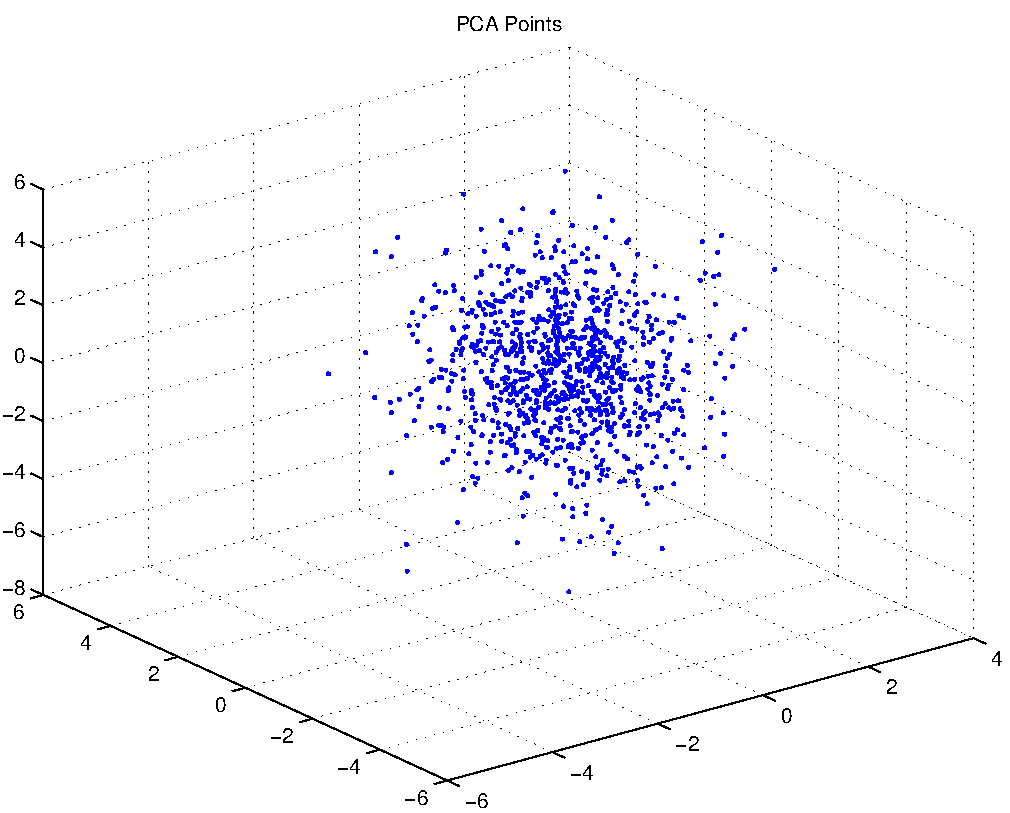
\includegraphics[width=10.0cm,height=10.0cm]{PCAPoints.pdf}

The eigenvectors:
+0.130, +0.312, +0.941
+0.178, +0.927, -0.332
-0.975, +0.210, +0.065

All of the eigenvalues of the covariance matrix:
(+0.958,+0.000), (+2.025,+0.000), (+3.017,+0.000)

QueryPerformanceCounter  =  +1.087
\subsubsection{Multi Variate Random Number Generator }
Sample from $N(\mu,\Sigma)$
mean= -0.002, variance=+1.004, skewness=+0.006, kurtosis=+3.003
mean= -0.001, variance=+1.017, skewness=-0.005, kurtosis=+2.988
mean= -0.002, variance=+1.006, skewness=-0.016, kurtosis=+3.014
Covariance Matrix 
+1.004, +0.009, +0.003
+0.009, +1.017, -0.003
+0.003, -0.003, +1.006

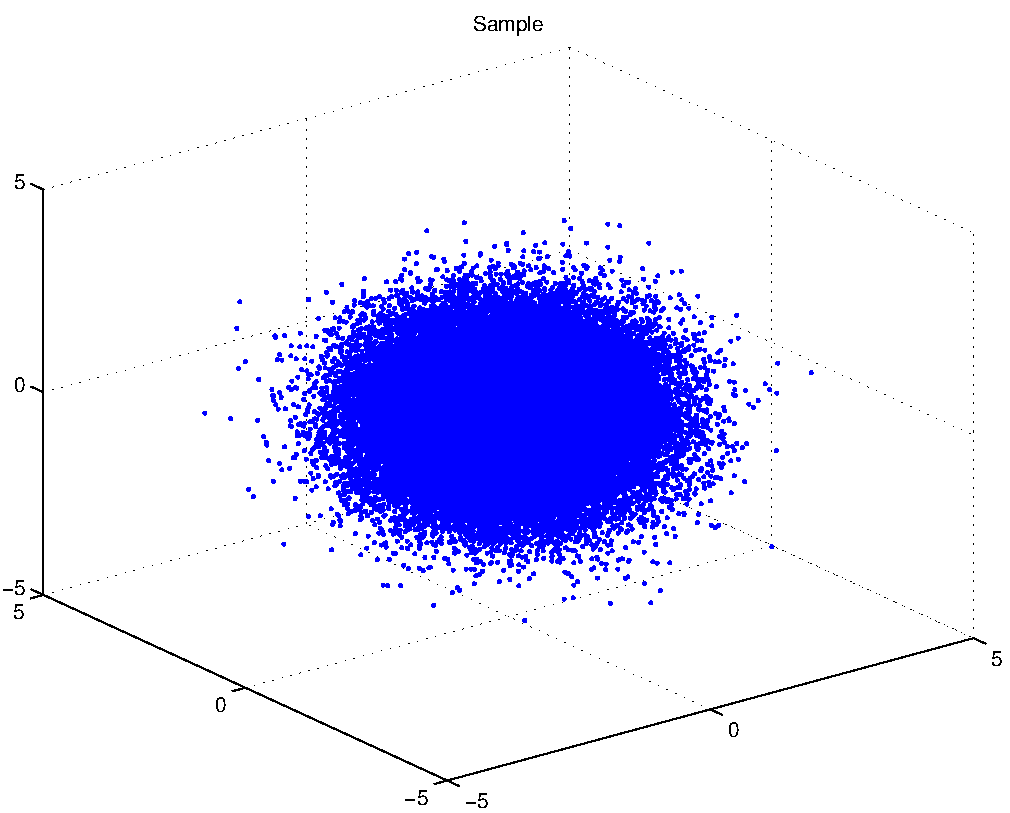
\includegraphics[width=10.0cm,height=10.0cm]{R_3_Normal.pdf}

Generate a sample from a unifom mixture of three Gaussians in $R^3$
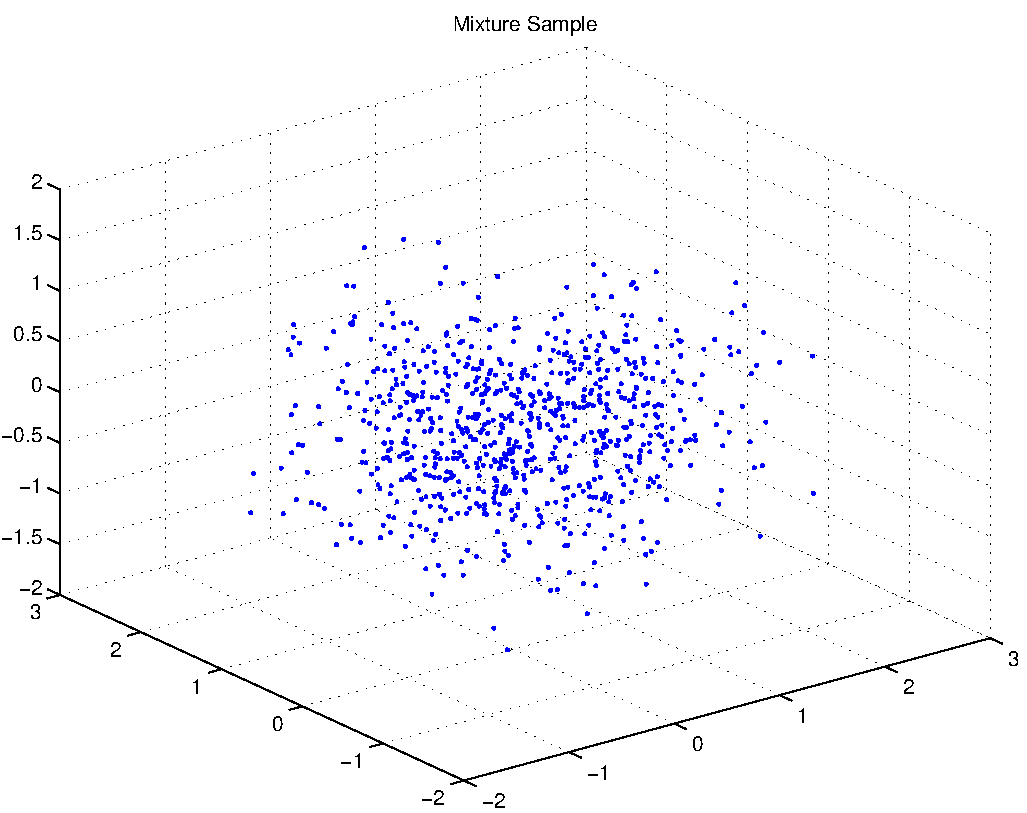
\includegraphics[width=10.0cm,height=10.0cm]{R_3_Normal_Mixture.pdf}

QueryPerformanceCounter  =  +16.605
\subsubsection{Matrix Multiply}
Comparing naive matrix multiply verus Intel MKL dgemm for matrix of size +2048.
This is for type double (hence the d in dgemm).
Naive type double matrix multiply tic toc  =  +0.387
dgemm plus row to column major transpose operation tic toc  =  +0.311
Comparing naive matrix multiply verus Intel MKL sgemm for matrix of size +2048.
This is for type float (hence the s in dgemm).
Naive type float matrix multiply tic toc  =  +0.253
sgemm plus row to column major transpose operation tic toc  =  +0.213
QueryPerformanceCounter  =  +1.290
\subsubsection{Descriptive Statistics}
Mean N(0,1): +0.003
Variance N(0,1): +1.006
Mean N(0,1) [recurrence relation method] :+0.003
Variance [recurrence relation method] :+1.006
Skewness : +0.007
Kurtosis : +2.997
QueryPerformanceCounter  =  +0.021
\subsubsection{Time Series }
+0.093
+0.726
+0.011
+2.178
QueryPerformanceCounter  =  +0.044
QueryPerformanceCounter  =  +6.353
\subsubsection{Iterated Exponential Filtering }
$\mu_1 =+0.093$
$\mu_2 =+0.726$
$\mu_3 =+0.011$
$\mu_4 =+2.178$
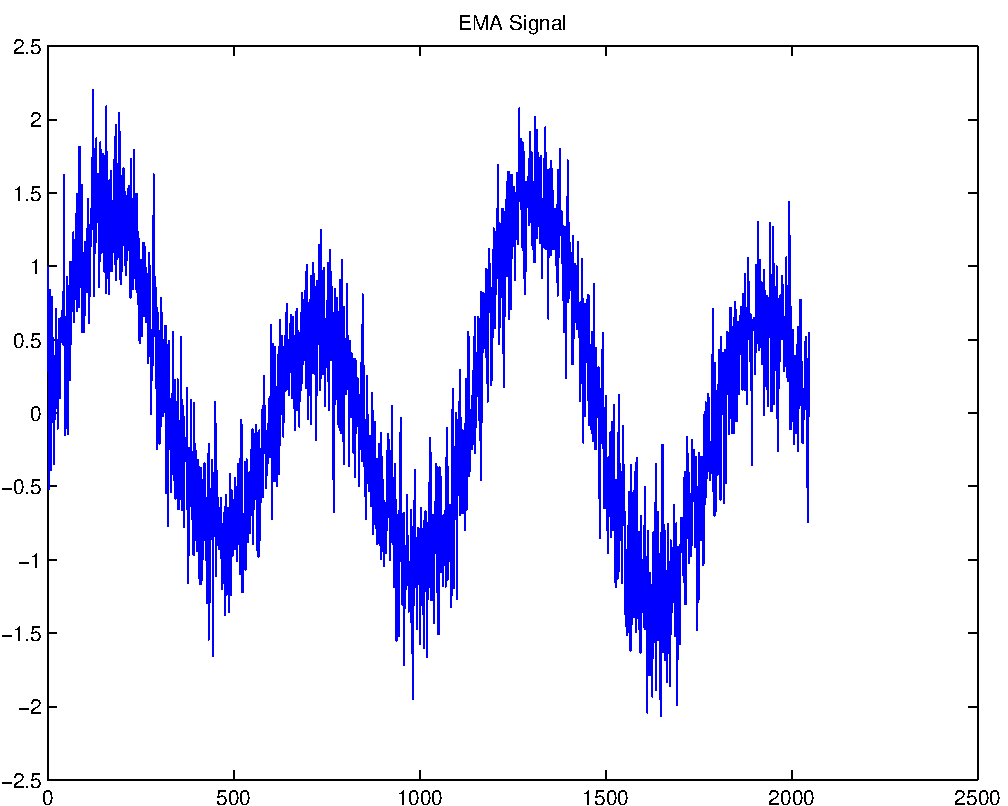
\includegraphics[width=10.0cm,height=10.0cm]{EMA_signal.pdf}

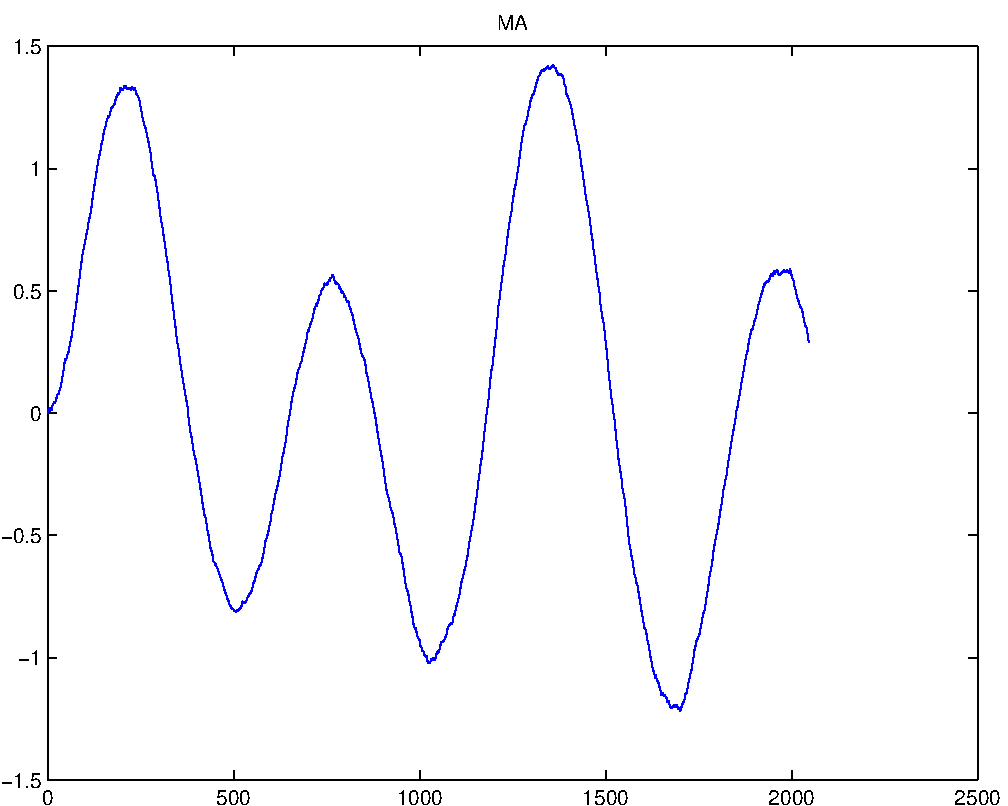
\includegraphics[width=10.0cm,height=10.0cm]{MA.pdf}

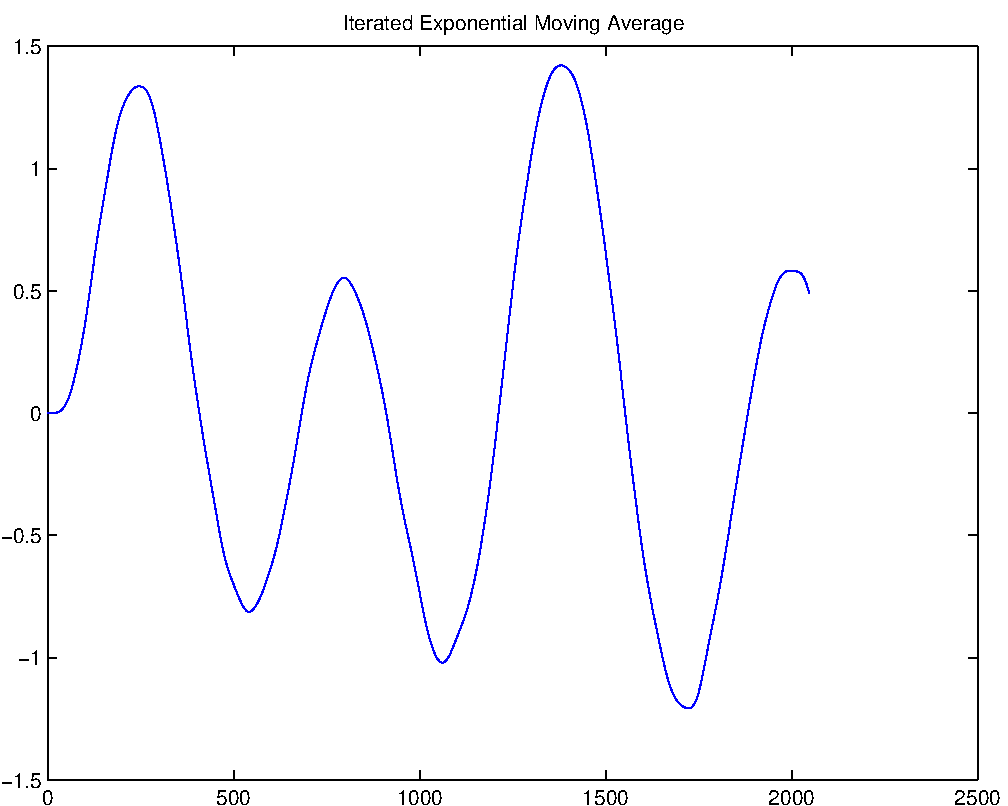
\includegraphics[width=10.0cm,height=10.0cm]{IEMA.pdf}

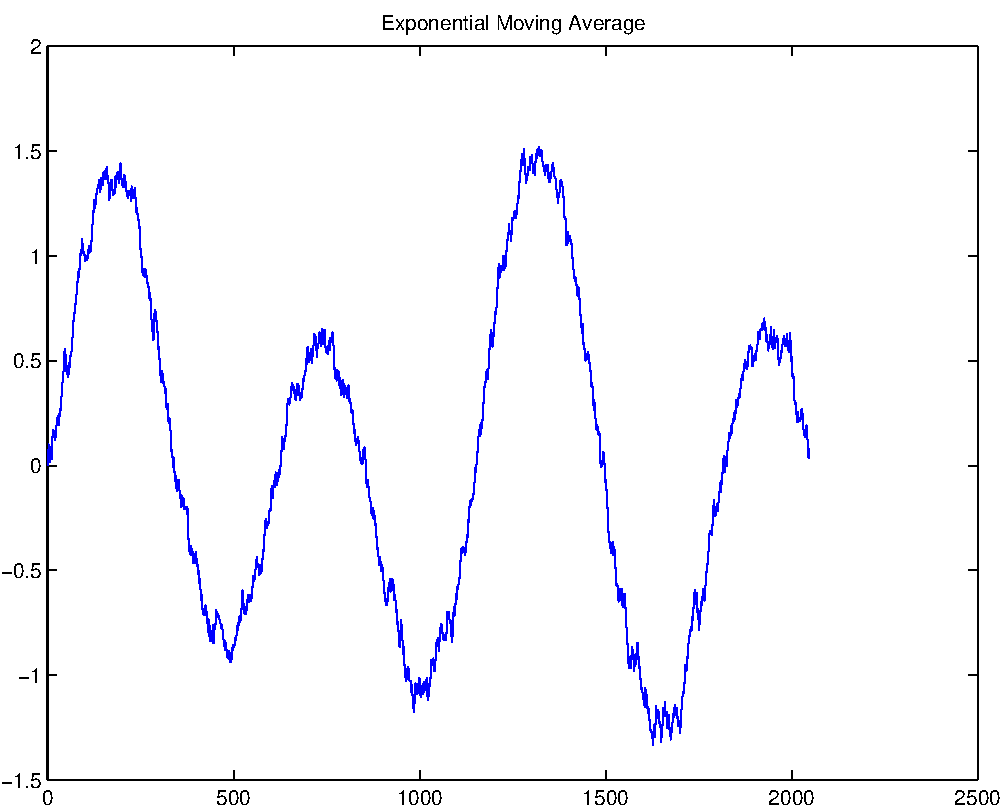
\includegraphics[width=10.0cm,height=10.0cm]{EMA.pdf}

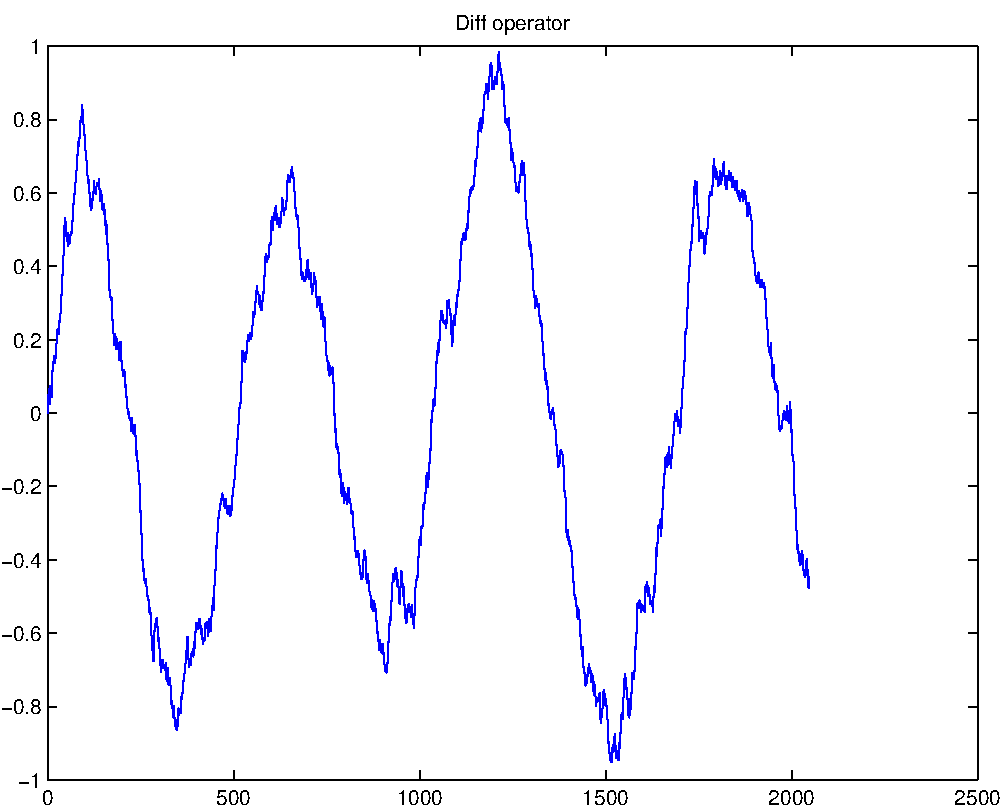
\includegraphics[width=10.0cm,height=10.0cm]{DIFF.pdf}

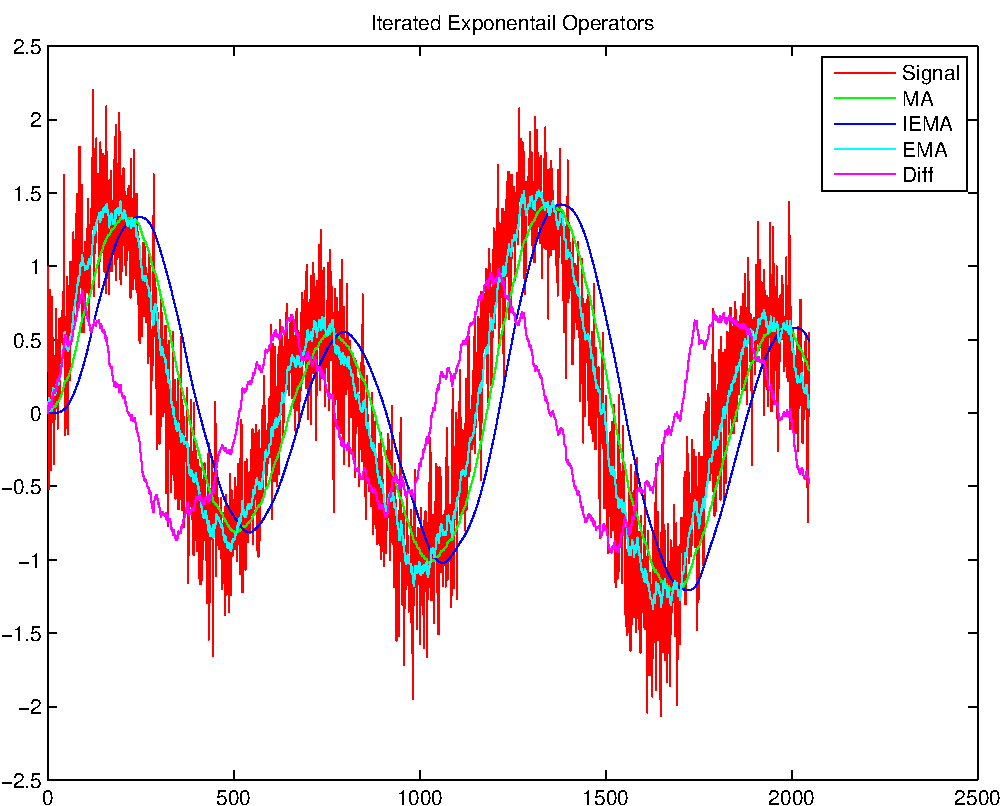
\includegraphics[width=10.0cm,height=10.0cm]{IteratedExponentailOperators.pdf}

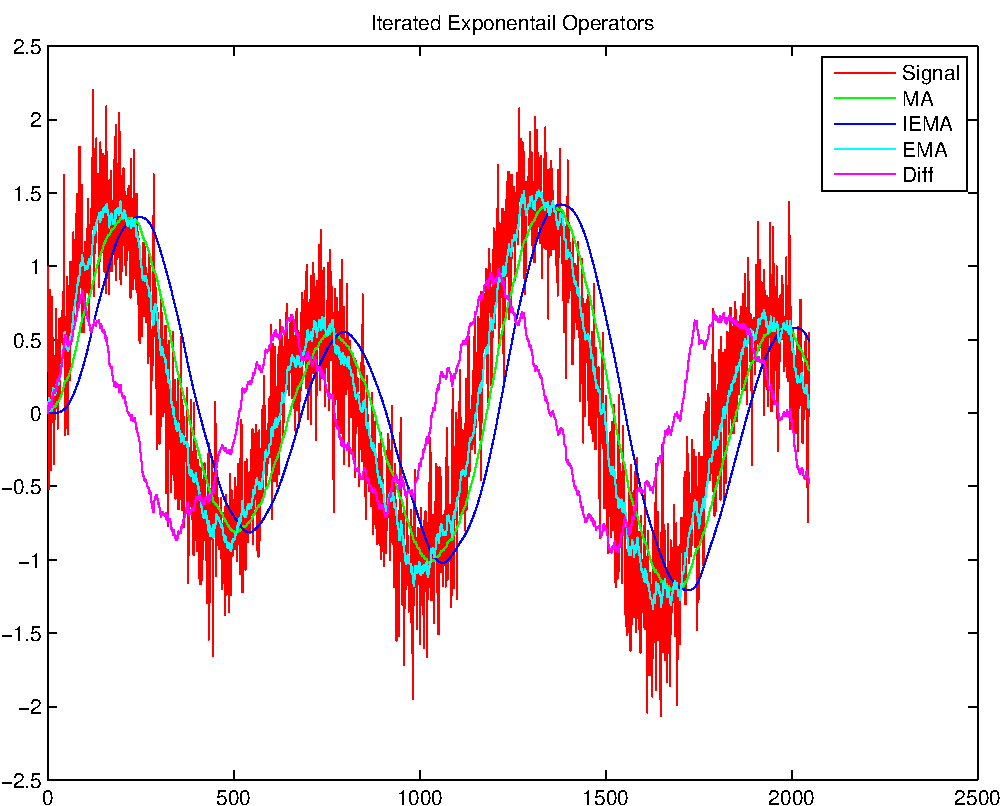
\includegraphics[width=10.0cm,height=10.0cm]{IteratedExponentailOperators.pdf}

QueryPerformanceCounter  =  +8.264
\subsubsection{Testing binary writer}
Binary writer Speedup 1GB Double Matrix +45.561

Binary reader Speedup 1GB Double Matrix +180.798

Binary writer Speedup 1GB Double vector +5.350

Binary reader Speedup 1GB Double Matrix +190.140

QueryPerformanceCounter  =  +0.908
\subsubsection{Testing Gaussian Mixture Point Cloud and Latex Plotting Capabilities.}
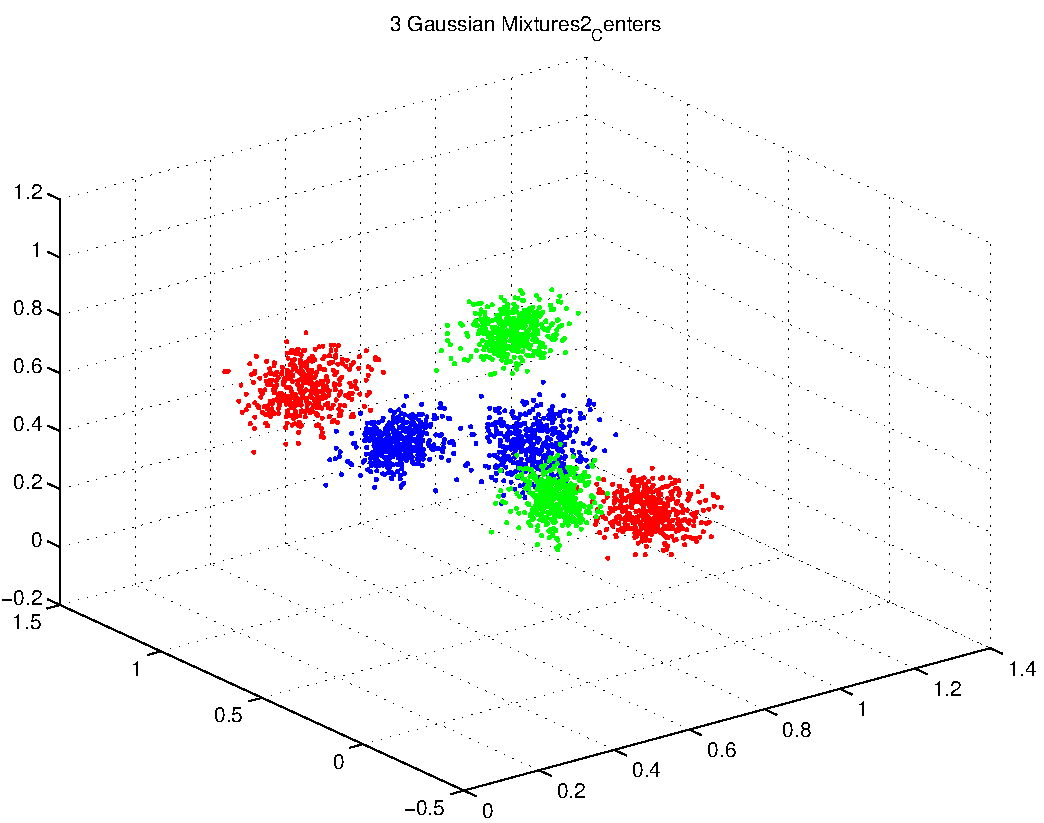
\includegraphics[width=10.0cm,height=10.0cm]{GaussianMixture_Dim_3_Centers2.pdf}

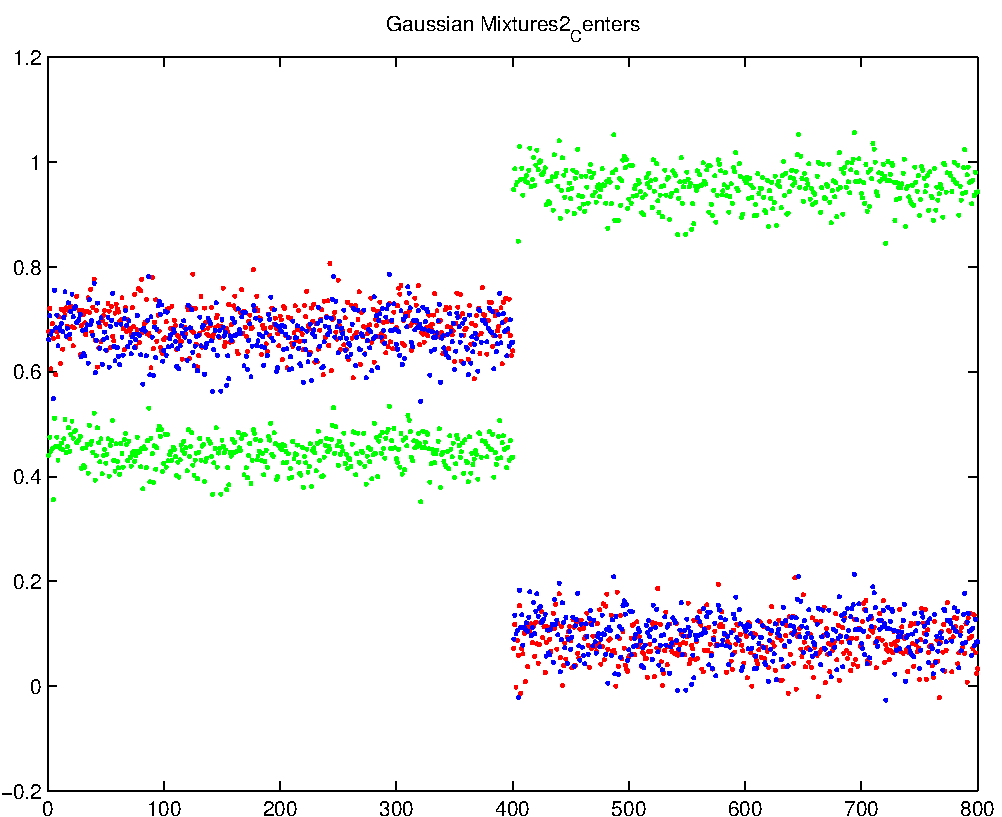
\includegraphics[width=10.0cm,height=10.0cm]{GaussianMixture_Dim_1_Centers2.pdf}

QueryPerformanceCounter  =  +2.898
\subsubsection{Intel VSL Function Check}
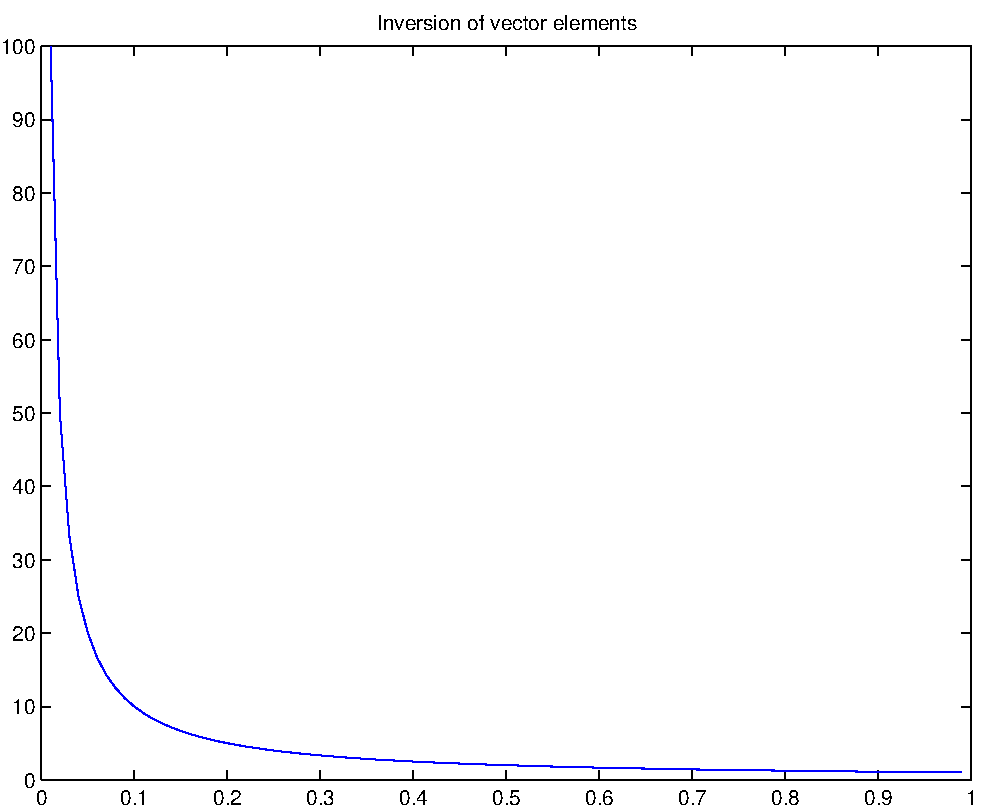
\includegraphics[width=10.0cm,height=10.0cm]{klVSLInv.pdf}

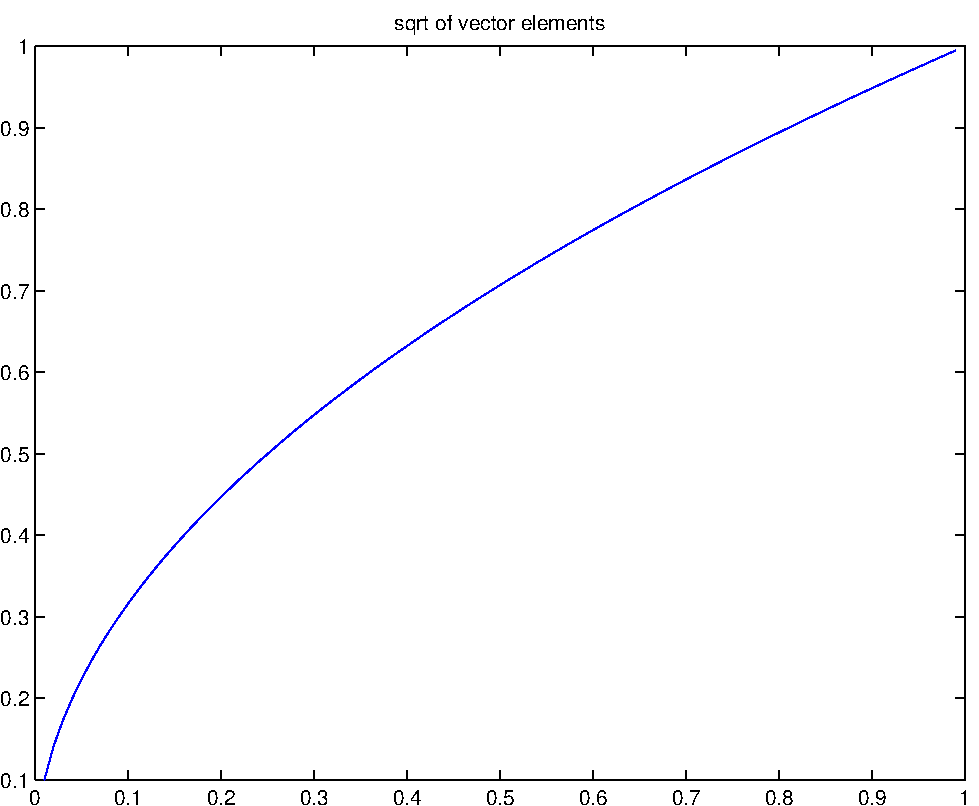
\includegraphics[width=10.0cm,height=10.0cm]{klVSLSqrt.pdf}

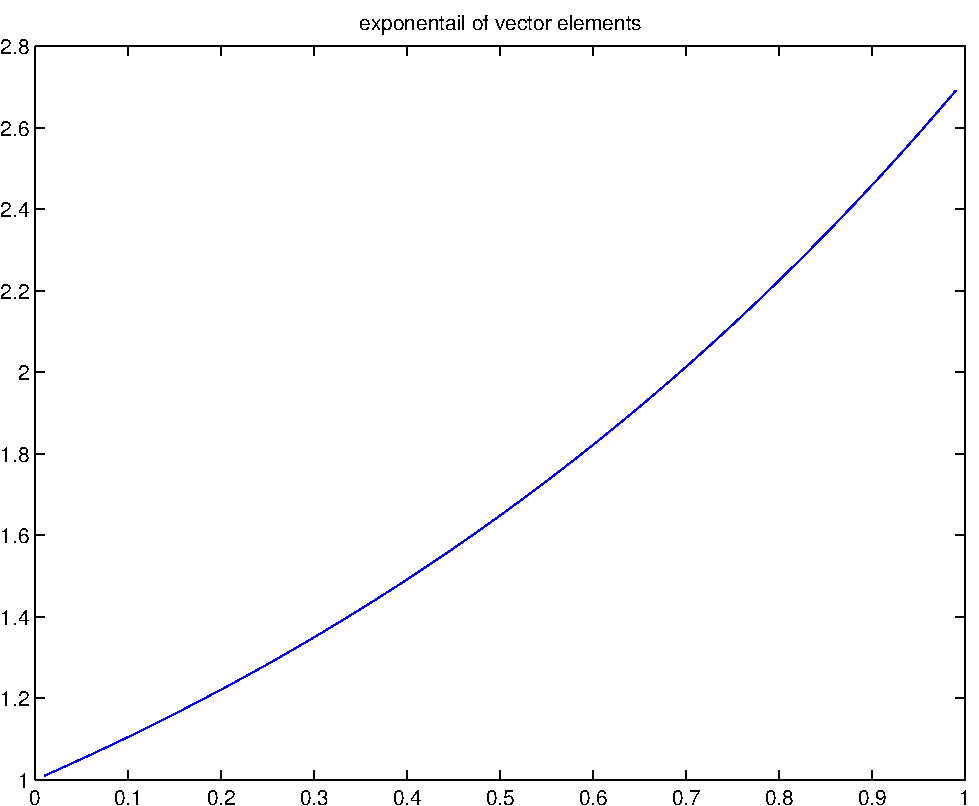
\includegraphics[width=10.0cm,height=10.0cm]{klVSLExp.pdf}

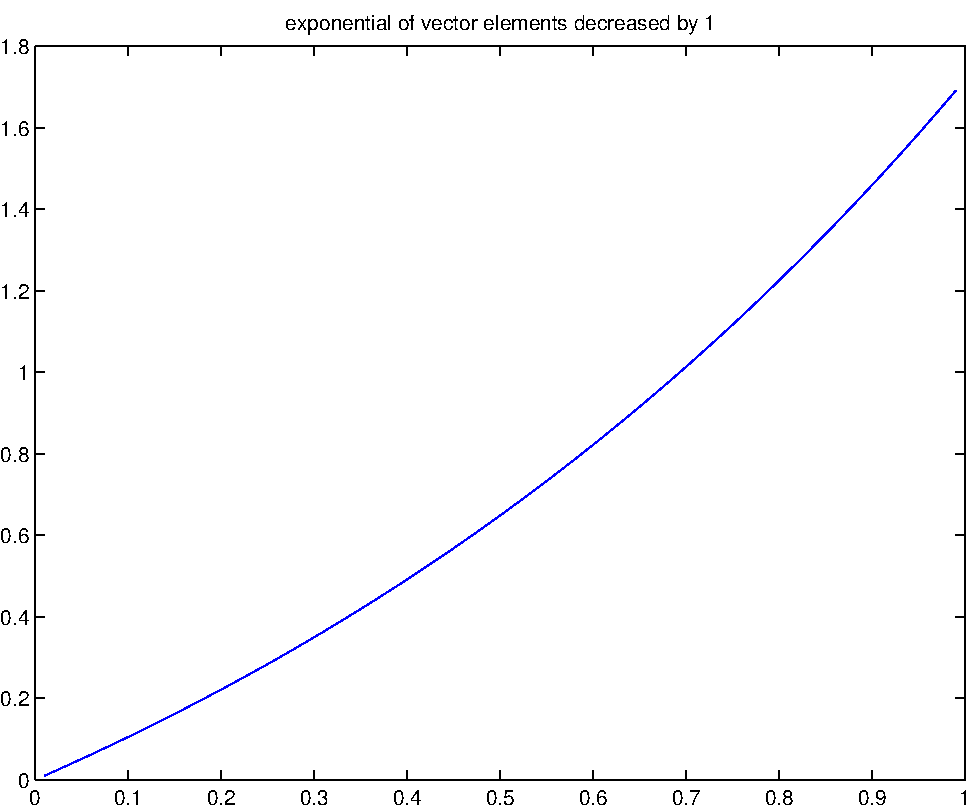
\includegraphics[width=10.0cm,height=10.0cm]{klVSLExpm1.pdf}

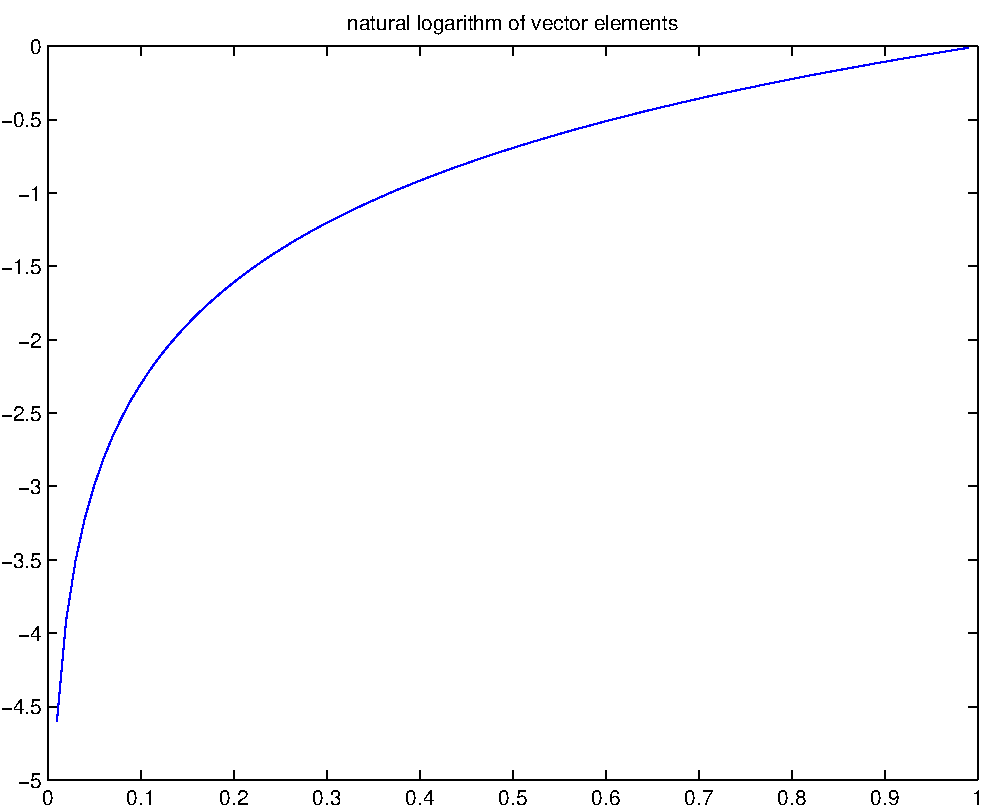
\includegraphics[width=10.0cm,height=10.0cm]{klVSLLn.pdf}

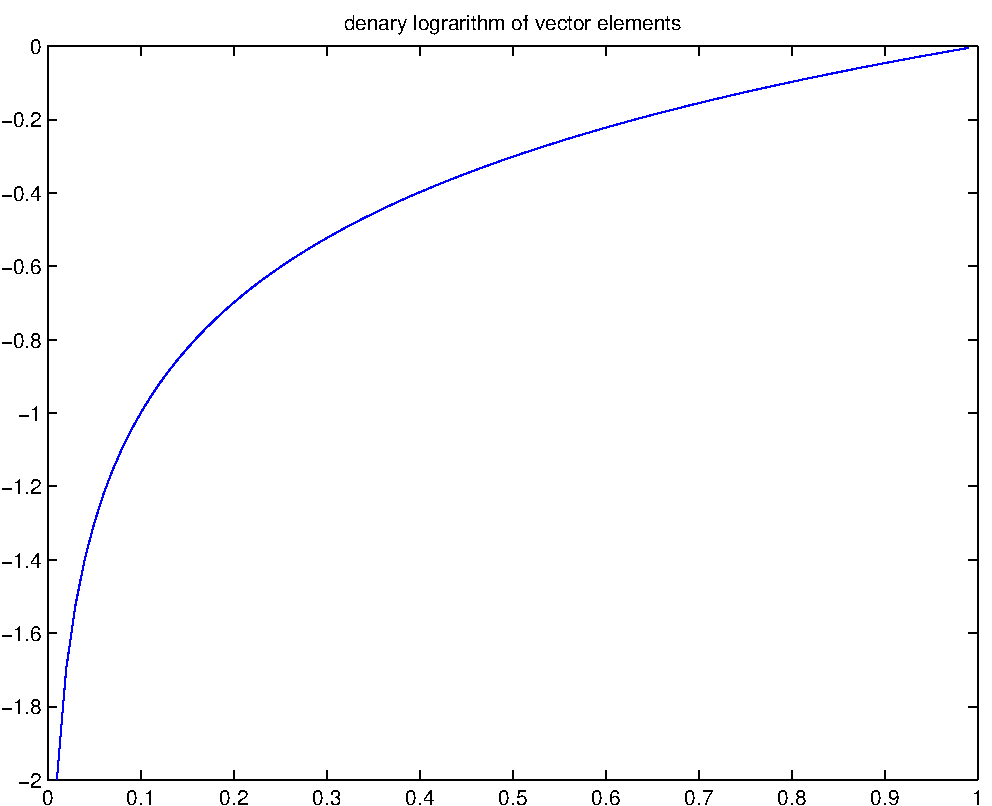
\includegraphics[width=10.0cm,height=10.0cm]{klVSLLog10.pdf}

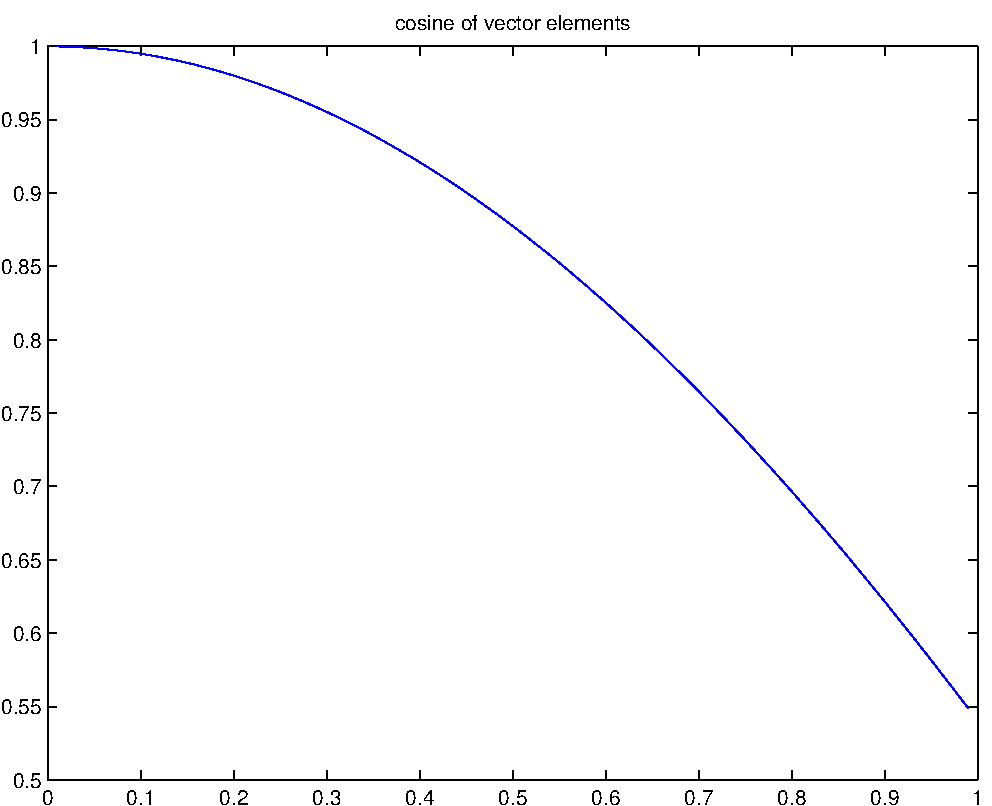
\includegraphics[width=10.0cm,height=10.0cm]{klVSLCos.pdf}

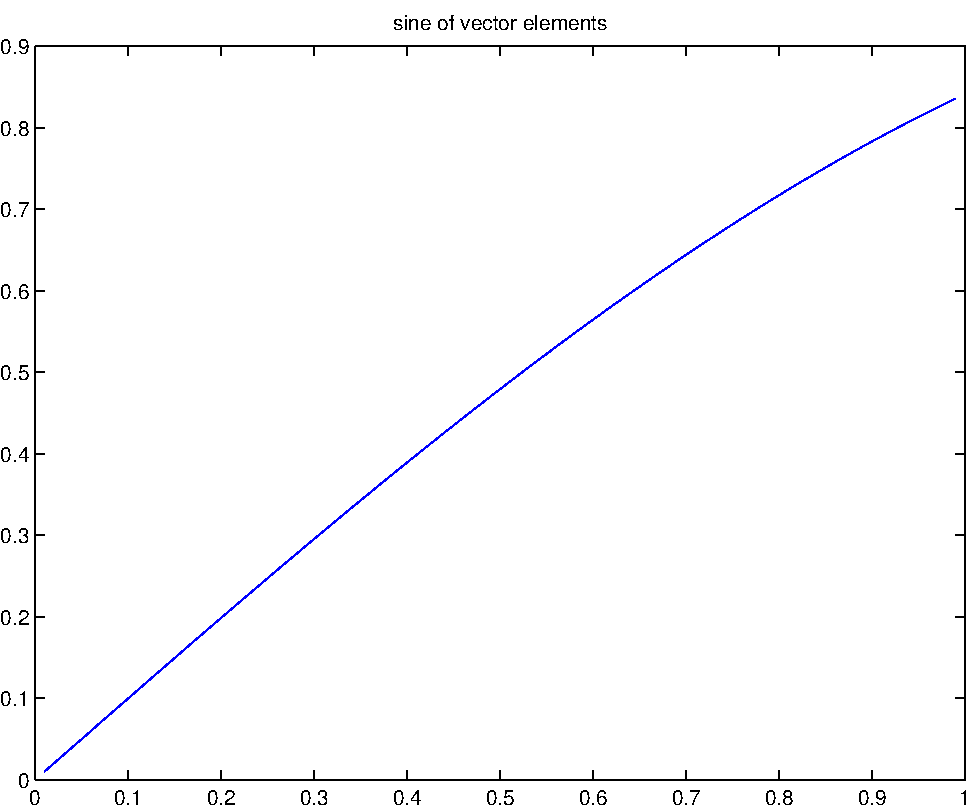
\includegraphics[width=10.0cm,height=10.0cm]{klVSLSin.pdf}

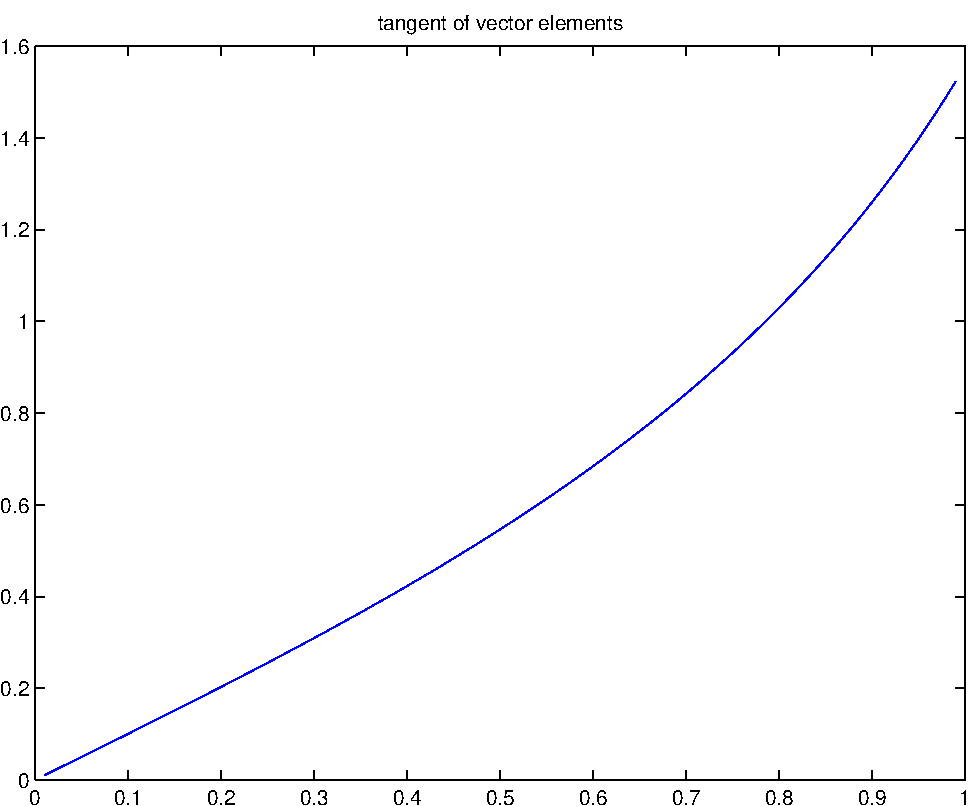
\includegraphics[width=10.0cm,height=10.0cm]{klVSLTan.pdf}

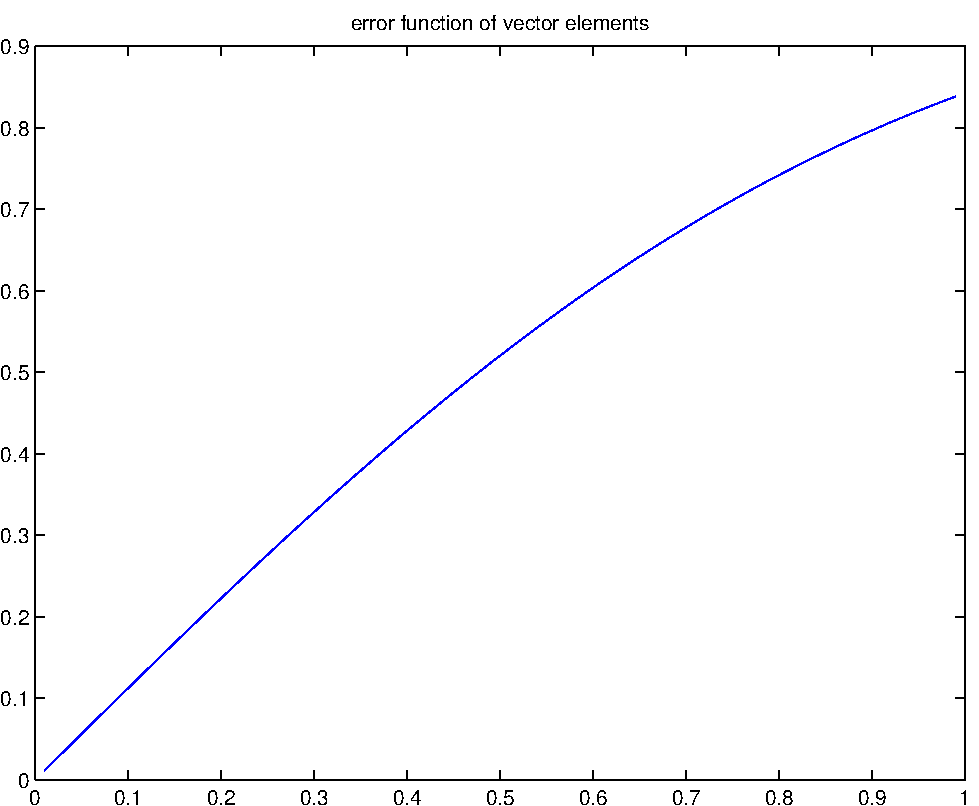
\includegraphics[width=10.0cm,height=10.0cm]{klVSLErf.pdf}

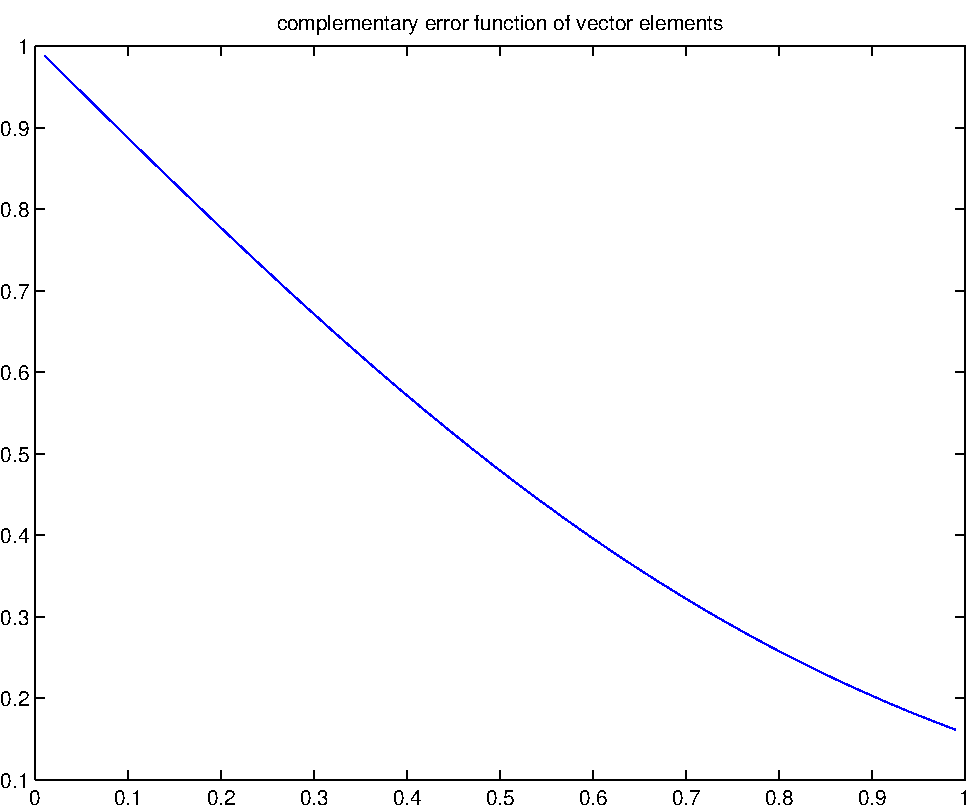
\includegraphics[width=10.0cm,height=10.0cm]{klVSLErfc.pdf}

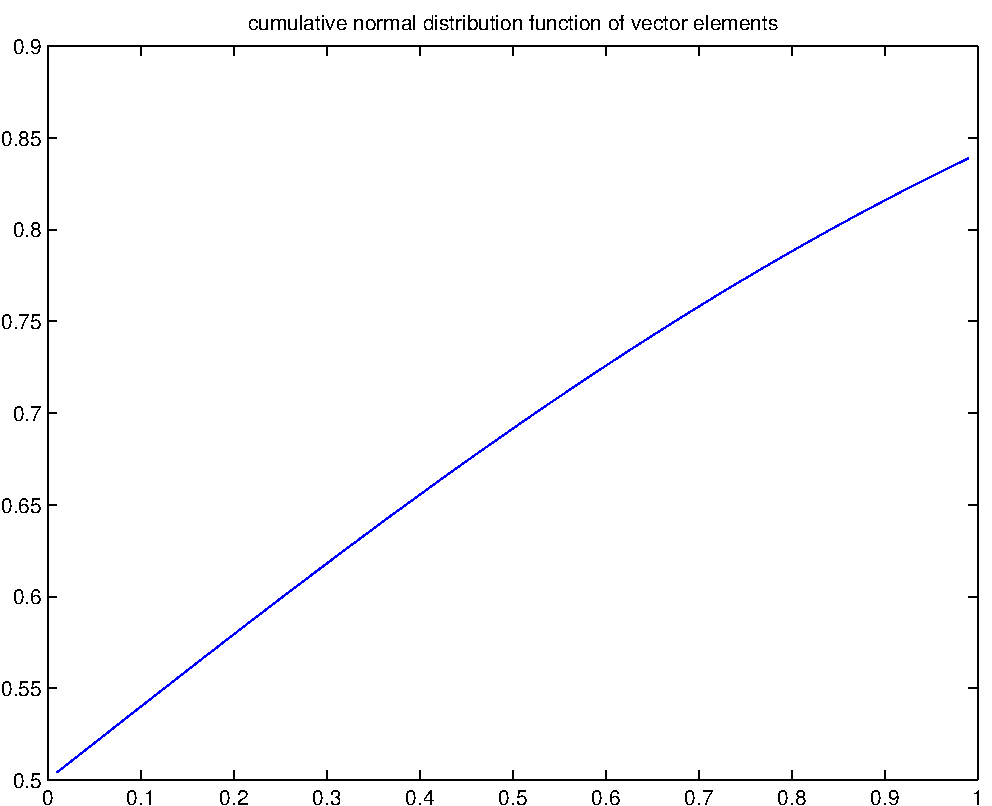
\includegraphics[width=10.0cm,height=10.0cm]{klVSLCdfNorm.pdf}

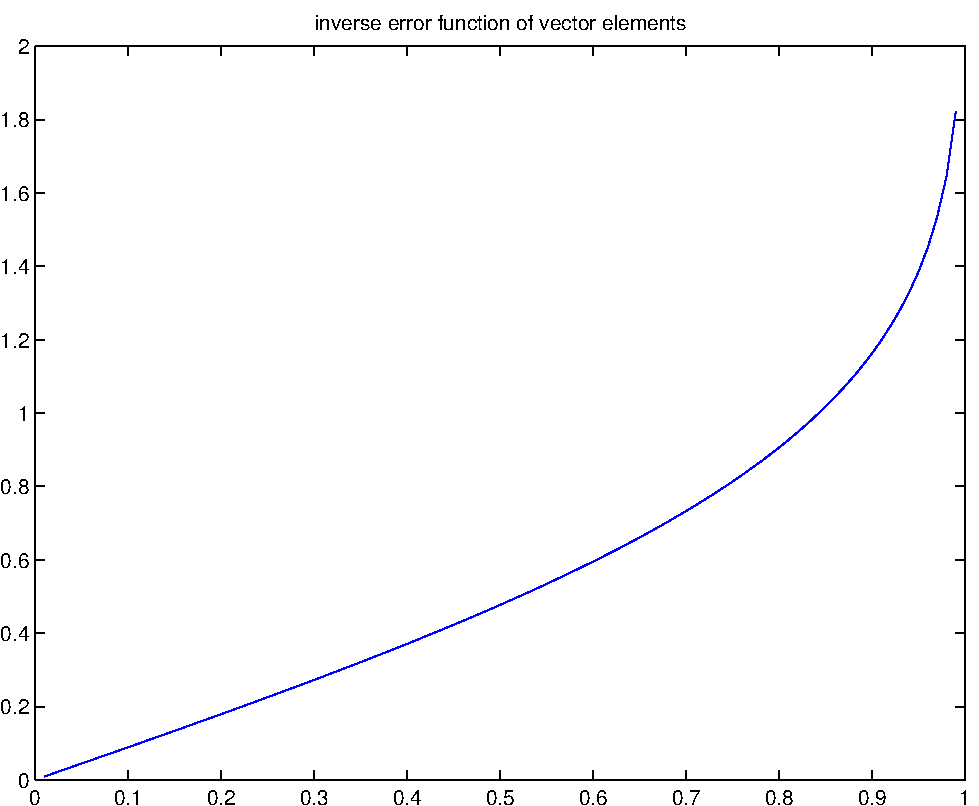
\includegraphics[width=10.0cm,height=10.0cm]{klVSLErfInv.pdf}

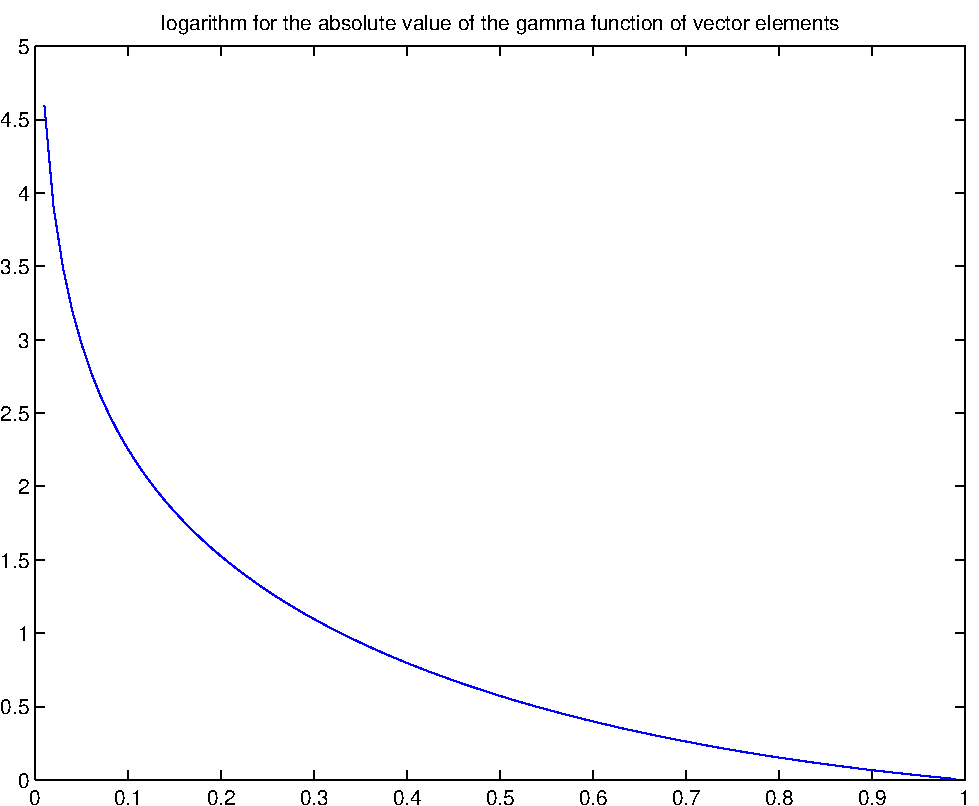
\includegraphics[width=10.0cm,height=10.0cm]{klVSLLGamma.pdf}

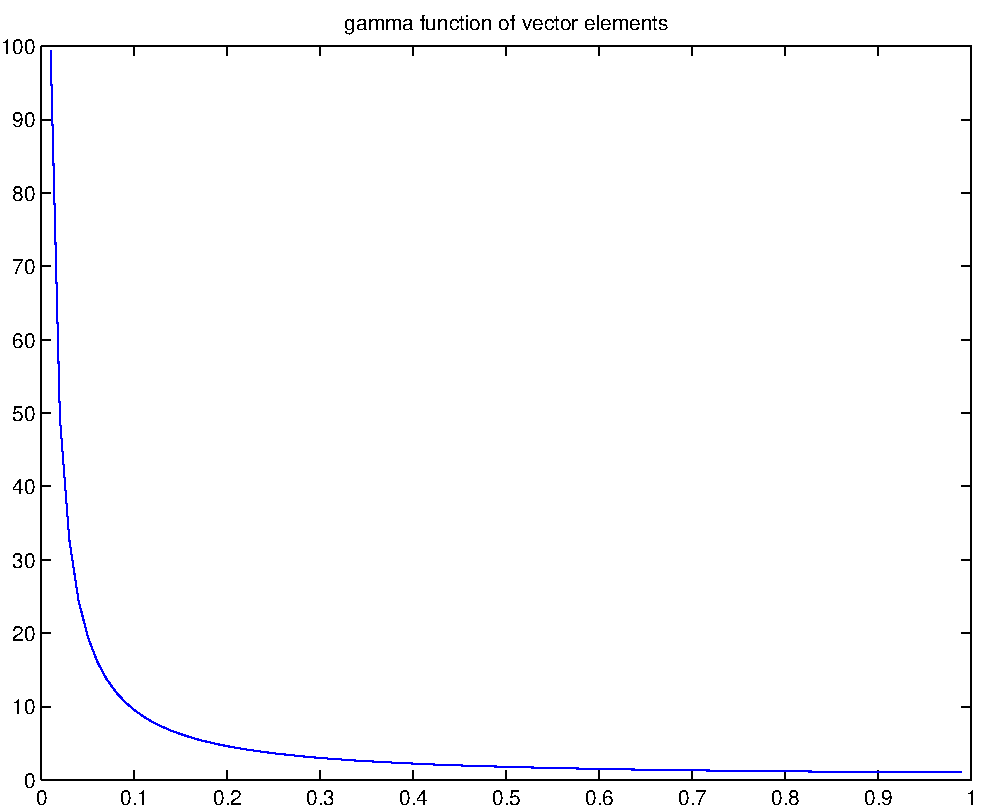
\includegraphics[width=10.0cm,height=10.0cm]{klVSLTGamma.pdf}

QueryPerformanceCounter  =  +14.153
\subsubsection{Gram Matrix Consistency Check}
Sample Size = 4096
Feature dim = 3

$$Sigma$ = \left(
\begin{array}{
ccc}
+1.140 & +1.535 & +0.581 \\
+1.535 & +9.988 & +1.605 \\
+0.581 & +1.605 & +0.428 \\
\end{array}
\right)$ \newline 

$Sample Covariance = \left(
\begin{array}{
ccc}
+1.153 & +1.590 & +0.599 \\
+1.590 & +10.053 & +1.649 \\
+0.599 & +1.649 & +0.444 \\
\end{array}
\right)$ \newline 

$Sample Mean = \left(
\begin{array}{
ccc}
+1.00515 & +1.00962 & +1.00407 \\
\end{array}
\right)$ \newline 

$Sample Covariance-$Omega$ = \left(
\begin{array}{
ccc}
+0.013 & +0.055 & +0.017 \\
+0.055 & +0.065 & +0.043 \\
+0.017 & +0.043 & +0.016 \\
\end{array}
\right)$ \newline 

$Sample Covariance Eigs = \left(
\begin{array}{
ccc}
(+10.62183,+0.00000) & (+0.98708,+0.00000) & (+0.04018,+0.00000) \\
\end{array}
\right)$ \newline 

$Centered Mean = \left(
\begin{array}{
ccc}
-0.00000 & -0.00000 & -0.00000 \\
\end{array}
\right)$ \newline 

$Centered Covariance = \left(
\begin{array}{
ccc}
+1.153 & +1.590 & +0.599 \\
+1.590 & +10.053 & +1.649 \\
+0.599 & +1.649 & +0.444 \\
\end{array}
\right)$ \newline 

$Gram Matrix Gf Not scaled by sample size = \left(
\begin{array}{
ccc}
+4720.734 & +6511.864 & +2451.199 \\
+6511.864 & +41177.080 & +6751.978 \\
+2451.199 & +6751.978 & +1816.834 \\
\end{array}
\right)$ \newline 

$Gram Matrix Gf  scaled by sample size = \left(
\begin{array}{
ccc}
+1.153 & +1.590 & +0.598 \\
+1.590 & +10.053 & +1.648 \\
+0.598 & +1.648 & +0.444 \\
\end{array}
\right)$ \newline 

$SampleCovariance - Scaled Gf = \left(
\begin{array}{
ccc}
+0.000 & +0.000 & +0.000 \\
+0.000 & +0.002 & +0.000 \\
+0.000 & +0.000 & +0.000 \\
\end{array}
\right)$ \newline 

$EigenDecomp of SampleCovariance = \left(
\begin{array}{
ccc}
-0.174 & -0.970 & -0.167 \\
+0.915 & -0.222 & +0.336 \\
-0.363 & -0.095 & +0.927 \\
\end{array}
\right)$ \newline 

$EigenDecomp of Gram Matrix = \left(
\begin{array}{
ccc}
-0.121 & -0.974 & -0.190 \\
-0.326 & +0.220 & -0.919 \\
+0.938 & -0.050 & -0.344 \\
\end{array}
\right)$ \newline 

QueryPerformanceCounter  =  +1.191
\subsubsection{Eigen Solver Checks}
\subsubsection{Haar Distributed Random Orthogonal Matrix $A \in O(n)$}
 Testing Operator Norm
Number of Dimensions: +8

$A = \left(
\begin{array}{
cccccccc}
+0.541 & +0.173 & -0.001 & -0.352 & +0.058 & +0.295 & +0.128 & -0.668 \\
-0.257 & +0.518 & +0.153 & +0.401 & +0.153 & +0.319 & -0.548 & -0.237 \\
+0.191 & -0.528 & +0.159 & -0.252 & +0.101 & -0.124 & -0.754 & -0.040 \\
+0.088 & -0.306 & +0.762 & +0.258 & +0.263 & +0.305 & +0.292 & +0.067 \\
-0.648 & -0.214 & +0.225 & -0.168 & -0.291 & -0.174 & +0.108 & -0.573 \\
+0.375 & -0.011 & +0.165 & +0.426 & -0.792 & -0.113 & -0.089 & -0.060 \\
-0.096 & +0.348 & +0.382 & -0.611 & -0.354 & +0.247 & -0.093 & +0.395 \\
-0.164 & -0.404 & -0.384 & +0.046 & -0.240 & +0.774 & -0.018 & +0.056 \\
\end{array}
\right)$ \newline 

$Det(A) :   A \in O(n)$ = (+1.000,+0.000)

$L = \left(
\begin{array}{
cccccccc}
+1.000 & +0.000 & +0.000 & +0.000 & +0.000 & +0.000 & +0.000 & +0.000 \\
+0.397 & +1.000 & +0.000 & +0.000 & +0.000 & +0.000 & +0.000 & +0.000 \\
-0.136 & -0.556 & +1.000 & +0.000 & +0.000 & +0.000 & +0.000 & +0.000 \\
+0.147 & +0.631 & +0.373 & +1.000 & +0.000 & +0.000 & +0.000 & +0.000 \\
-0.578 & -0.224 & +0.374 & -0.233 & +1.000 & +0.000 & +0.000 & +0.000 \\
+0.254 & -0.580 & -0.489 & -0.566 & +0.151 & +1.000 & +0.000 & +0.000 \\
-0.295 & -0.981 & +0.348 & +0.014 & -0.133 & -0.010 & +1.000 & +0.000 \\
-0.835 & -0.008 & +0.226 & +0.564 & -0.069 & +0.084 & -0.060 & +1.000 \\
\end{array}
\right)$ \newline 

$U = \left(
\begin{array}{
cccccccc}
-0.648 & -0.214 & +0.225 & -0.168 & -0.291 & -0.174 & +0.108 & -0.573 \\
+0.000 & +0.602 & +0.064 & +0.468 & +0.268 & +0.388 & -0.591 & -0.010 \\
+0.000 & +0.000 & +0.828 & +0.496 & +0.372 & +0.497 & -0.022 & -0.016 \\
+0.000 & +0.000 & +0.000 & -1.066 & -0.619 & -0.157 & +0.273 & +0.491 \\
+0.000 & +0.000 & +0.000 & +0.000 & -1.183 & -0.349 & -0.087 & -0.273 \\
+0.000 & +0.000 & +0.000 & +0.000 & +0.000 & +1.250 & -0.232 & +0.507 \\
+0.000 & +0.000 & +0.000 & +0.000 & +0.000 & +0.000 & -1.312 & -0.252 \\
+0.000 & +0.000 & +0.000 & +0.000 & +0.000 & +0.000 & +0.000 & -1.497 \\
\end{array}
\right)$ \newline 

$L * U  = \left(
\begin{array}{
cccccccc}
-0.648 & -0.214 & +0.225 & -0.168 & -0.291 & -0.174 & +0.108 & -0.573 \\
-0.257 & +0.518 & +0.153 & +0.401 & +0.153 & +0.319 & -0.548 & -0.237 \\
+0.088 & -0.306 & +0.762 & +0.258 & +0.263 & +0.305 & +0.292 & +0.067 \\
-0.096 & +0.348 & +0.382 & -0.611 & -0.354 & +0.247 & -0.093 & +0.395 \\
+0.375 & -0.011 & +0.165 & +0.426 & -0.792 & -0.113 & -0.089 & -0.060 \\
-0.164 & -0.404 & -0.384 & +0.046 & -0.240 & +0.774 & -0.018 & +0.056 \\
+0.191 & -0.528 & +0.159 & -0.252 & +0.101 & -0.124 & -0.754 & -0.040 \\
+0.541 & +0.173 & -0.001 & -0.352 & +0.058 & +0.295 & +0.128 & -0.668 \\
\end{array}
\right)$ \newline 

$Det(L) :    = (+1.000,+0.000)     Det(U) :    = (-1.000,+0.000)     Det(LU) :    = (-1.000,+0.000)$

$||A||_{L_1}$  = +2.515

$||A||_{L_{\infty}}$ = +2.586

$||A^{-1}||_{L_1}$  = +2.586

$||A^{-1}||_{L_{\infty}}$ = +2.515

$||A||_{L_{\infty}} * ||A^{-1}||_{L_{\infty}} = +6.503$

$||A||_{L_1} * ||A^{-1}||_{L_1} = +6.503$

Frobenious Norm  $||A||_{\textit{F}}$ via $\sum\limits_{i,j =0}^{n} \|A_{i,j}|$   of  $A \in O(n)$  +2.828

$L_1$ condition number of Haar Distributed Random Orthogonal Matrix $A \in O(n)$ +5.405

$A = \left(
\begin{array}{
cccccccc}
+0.541 & +0.173 & -0.001 & -0.352 & +0.058 & +0.295 & +0.128 & -0.668 \\
-0.257 & +0.518 & +0.153 & +0.401 & +0.153 & +0.319 & -0.548 & -0.237 \\
+0.191 & -0.528 & +0.159 & -0.252 & +0.101 & -0.124 & -0.754 & -0.040 \\
+0.088 & -0.306 & +0.762 & +0.258 & +0.263 & +0.305 & +0.292 & +0.067 \\
-0.648 & -0.214 & +0.225 & -0.168 & -0.291 & -0.174 & +0.108 & -0.573 \\
+0.375 & -0.011 & +0.165 & +0.426 & -0.792 & -0.113 & -0.089 & -0.060 \\
-0.096 & +0.348 & +0.382 & -0.611 & -0.354 & +0.247 & -0.093 & +0.395 \\
-0.164 & -0.404 & -0.384 & +0.046 & -0.240 & +0.774 & -0.018 & +0.056 \\
\end{array}
\right)$ \newline 

$L_{\infty}$ condition number of Haar Distributed Random Orthogonal Matrix $A \in O(n)$ +6.468

Eigenvalues of $A \in O(n)$

(-0.781,+0.625), (-0.781,-0.625), (-0.236,+0.972), (-0.236,-0.972), (+0.637,+0.771), (+0.637,-0.771), (+0.897,+0.442), (+0.897,-0.442)

 $|\lambda | : \lambda \in \sigma(A) , A \in O(n)$

+1.000, +1.000, +1.000, +1.000, +1.000, +1.000, +1.000, +1.000


Calculating $A^{\dag} A,$  we expect $A^{\dag} A \approx I$

$A^{\dag} A = \left(
\begin{array}{
cccccccc}
+1.000 & -0.000 & -0.000 & -0.000 & +0.000 & +0.000 & +0.000 & +0.000 \\
-0.000 & +1.000 & -0.000 & +0.000 & +0.000 & +0.000 & -0.000 & +0.000 \\
-0.000 & -0.000 & +1.000 & +0.000 & -0.000 & +0.000 & +0.000 & -0.000 \\
-0.000 & +0.000 & +0.000 & +1.000 & +0.000 & +0.000 & -0.000 & +0.000 \\
+0.000 & +0.000 & -0.000 & +0.000 & +1.000 & +0.000 & -0.000 & +0.000 \\
+0.000 & +0.000 & +0.000 & +0.000 & +0.000 & +1.000 & -0.000 & +0.000 \\
+0.000 & -0.000 & +0.000 & -0.000 & -0.000 & -0.000 & +1.000 & +0.000 \\
+0.000 & +0.000 & -0.000 & +0.000 & +0.000 & +0.000 & +0.000 & +1.000 \\
\end{array}
\right)$ \newline 

Calculating $A^{-1} ,  A \in O(n)$.

$A^{-1} = \left(
\begin{array}{
cccccccc}
+0.541 & -0.257 & +0.191 & +0.088 & -0.648 & +0.375 & -0.096 & -0.164 \\
+0.173 & +0.518 & -0.528 & -0.306 & -0.214 & -0.011 & +0.348 & -0.404 \\
-0.001 & +0.153 & +0.159 & +0.762 & +0.225 & +0.165 & +0.382 & -0.384 \\
-0.352 & +0.401 & -0.252 & +0.258 & -0.168 & +0.426 & -0.611 & +0.046 \\
+0.058 & +0.153 & +0.101 & +0.263 & -0.291 & -0.792 & -0.354 & -0.240 \\
+0.295 & +0.319 & -0.124 & +0.305 & -0.174 & -0.113 & +0.247 & +0.774 \\
+0.128 & -0.548 & -0.754 & +0.292 & +0.108 & -0.089 & -0.093 & -0.018 \\
-0.668 & -0.237 & -0.040 & +0.067 & -0.573 & -0.060 & +0.395 & +0.056 \\
\end{array}
\right)$ \newline 

Calculating $A^{-1} *A  ,  A \in O(n)$.   We expect $A^{-1} *A  \approx I$. 

$A^{-1} *A = \left(
\begin{array}{
cccccccc}
+1.000 & -0.000 & +0.000 & -0.000 & -0.000 & +0.000 & -0.000 & +0.000 \\
-0.000 & +1.000 & -0.000 & +0.000 & +0.000 & -0.000 & +0.000 & -0.000 \\
+0.000 & -0.000 & +1.000 & +0.000 & +0.000 & +0.000 & -0.000 & +0.000 \\
-0.000 & -0.000 & +0.000 & +1.000 & +0.000 & +0.000 & +0.000 & +0.000 \\
-0.000 & -0.000 & +0.000 & +0.000 & +1.000 & +0.000 & -0.000 & -0.000 \\
+0.000 & -0.000 & +0.000 & +0.000 & +0.000 & +1.000 & +0.000 & -0.000 \\
-0.000 & +0.000 & -0.000 & -0.000 & -0.000 & -0.000 & +1.000 & +0.000 \\
+0.000 & +0.000 & -0.000 & -0.000 & +0.000 & +0.000 & +0.000 & +1.000 \\
\end{array}
\right)$ \newline 

Calculating SVD of  $A \in O(n)$

$U = \left(
\begin{array}{
cccccccc}
+0.731 & -0.069 & -0.260 & -0.053 & +0.263 & -0.236 & -0.036 & +0.514 \\
-0.113 & +0.785 & +0.138 & -0.318 & +0.093 & -0.361 & -0.328 & +0.066 \\
-0.018 & -0.215 & -0.188 & -0.549 & -0.523 & +0.280 & -0.471 & +0.207 \\
+0.256 & +0.269 & -0.205 & +0.677 & -0.382 & +0.091 & -0.428 & -0.155 \\
+0.214 & +0.157 & +0.746 & +0.091 & -0.103 & +0.459 & +0.068 & +0.372 \\
-0.220 & +0.308 & -0.459 & +0.035 & +0.416 & +0.652 & +0.029 & +0.213 \\
-0.019 & -0.333 & +0.261 & +0.054 & +0.561 & +0.064 & -0.681 & -0.185 \\
-0.541 & -0.173 & +0.001 & +0.352 & -0.058 & -0.295 & -0.128 & +0.668 \\
\end{array}
\right)$ \newline 

$S = \left(
\begin{array}{
cccccccc}
+1.000 & +0.000 & +0.000 & +0.000 & +0.000 & +0.000 & +0.000 & +0.000 \\
+0.000 & +1.000 & +0.000 & +0.000 & +0.000 & +0.000 & +0.000 & +0.000 \\
+0.000 & +0.000 & +1.000 & +0.000 & +0.000 & +0.000 & +0.000 & +0.000 \\
+0.000 & +0.000 & +0.000 & +1.000 & +0.000 & +0.000 & +0.000 & +0.000 \\
+0.000 & +0.000 & +0.000 & +0.000 & +1.000 & +0.000 & +0.000 & +0.000 \\
+0.000 & +0.000 & +0.000 & +0.000 & +0.000 & +1.000 & +0.000 & +0.000 \\
+0.000 & +0.000 & +0.000 & +0.000 & +0.000 & +0.000 & +1.000 & +0.000 \\
+0.000 & +0.000 & +0.000 & +0.000 & +0.000 & +0.000 & +0.000 & +1.000 \\
\end{array}
\right)$ \newline 

$V = \left(
\begin{array}{
cccccccc}
+0.000 & +0.000 & -0.000 & -0.000 & -0.000 & +0.000 & -0.000 & -1.000 \\
-0.422 & +0.392 & -0.137 & +0.556 & +0.182 & +0.365 & +0.418 & -0.000 \\
+0.211 & -0.035 & +0.478 & -0.017 & -0.080 & -0.355 & +0.770 & +0.000 \\
-0.105 & -0.404 & -0.396 & -0.250 & +0.720 & -0.124 & +0.268 & +0.000 \\
-0.843 & -0.048 & +0.042 & -0.245 & -0.275 & -0.386 & -0.009 & +0.000 \\
+0.000 & -0.172 & +0.143 & +0.687 & +0.241 & -0.565 & -0.317 & +0.000 \\
-0.105 & +0.465 & +0.570 & -0.286 & +0.554 & +0.027 & -0.240 & +0.000 \\
-0.211 & -0.659 & +0.499 & +0.121 & +0.019 & +0.506 & -0.043 & +0.000 \\
\end{array}
\right)$ \newline 

$U S V = \left(
\begin{array}{
cccccccc}
-0.346 & -0.324 & +0.119 & -0.174 & -0.170 & +0.365 & -0.185 & -0.731 \\
-0.326 & +0.293 & -0.118 & +0.344 & -0.390 & +0.470 & +0.538 & +0.113 \\
+0.556 & -0.235 & +0.010 & +0.501 & -0.465 & +0.192 & -0.362 & +0.018 \\
+0.172 & -0.256 & -0.727 & +0.244 & +0.440 & +0.094 & +0.220 & -0.256 \\
+0.083 & -0.288 & +0.584 & +0.419 & +0.218 & -0.249 & +0.488 & -0.214 \\
-0.629 & -0.136 & -0.042 & +0.534 & +0.181 & -0.149 & -0.442 & +0.220 \\
-0.173 & -0.394 & -0.299 & -0.124 & -0.563 & -0.586 & +0.223 & +0.019 \\
-0.042 & -0.657 & +0.100 & -0.255 & +0.108 & +0.416 & +0.119 & +0.541 \\
\end{array}
\right)$ \newline 

Calculating first few eigenvectors of $A \in O(n)$ using LAPACK syevx

\subsubsection{Wishart Matrix $A \in W(n)$}
$L_1$ condition number of Wishart Matrix +1489.694
$L_infty$ condition number of Wishart Matrix +1489.694
\subsubsection{Gaussian Orthogonal Ensemble $A \in GOE(n)$}
$L_1$ condition number of GOE Matrix +66.900
$L_\infty$ condition number of GOE Matrix +66.900
\subsubsection{The Identity Matrix $I \in M(n)$}
$L_1$ condition number of $I$ = +1.000
$L_\infty$ condition number of $I$ = +1.000
QueryPerformanceCounter  =  +0.275
\subsubsection{Generate Tracey Widom Sample}
\subsubsection{Sample from $W_n m$ times and calculate empirical PDF of the first eig}
Here we generate histograms of $\lambda_1$ for GOE (Gaussian Orthogonal Ensemble), and W (Wishart) 		 distributed of random matrices
These should approximate the celebrated Tracy Widom distribution.
Dimension $n = +128$

Sample size $m = 32$

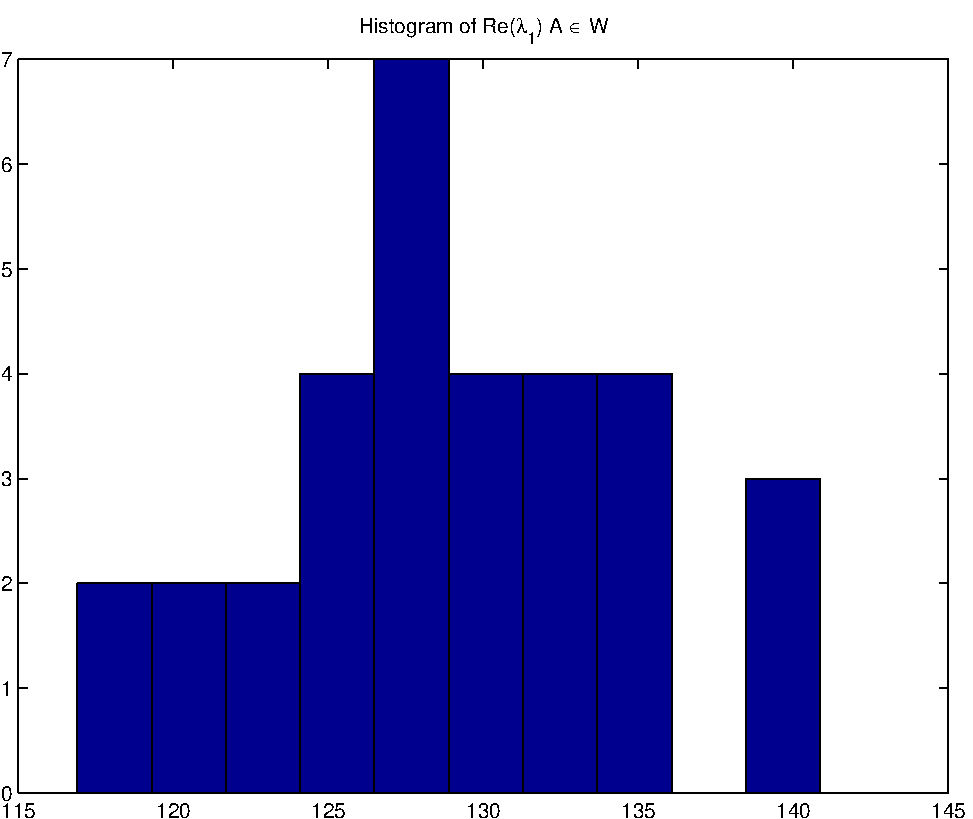
\includegraphics[width=10.0cm,height=10.0cm]{Re_TraceyWidom.pdf}

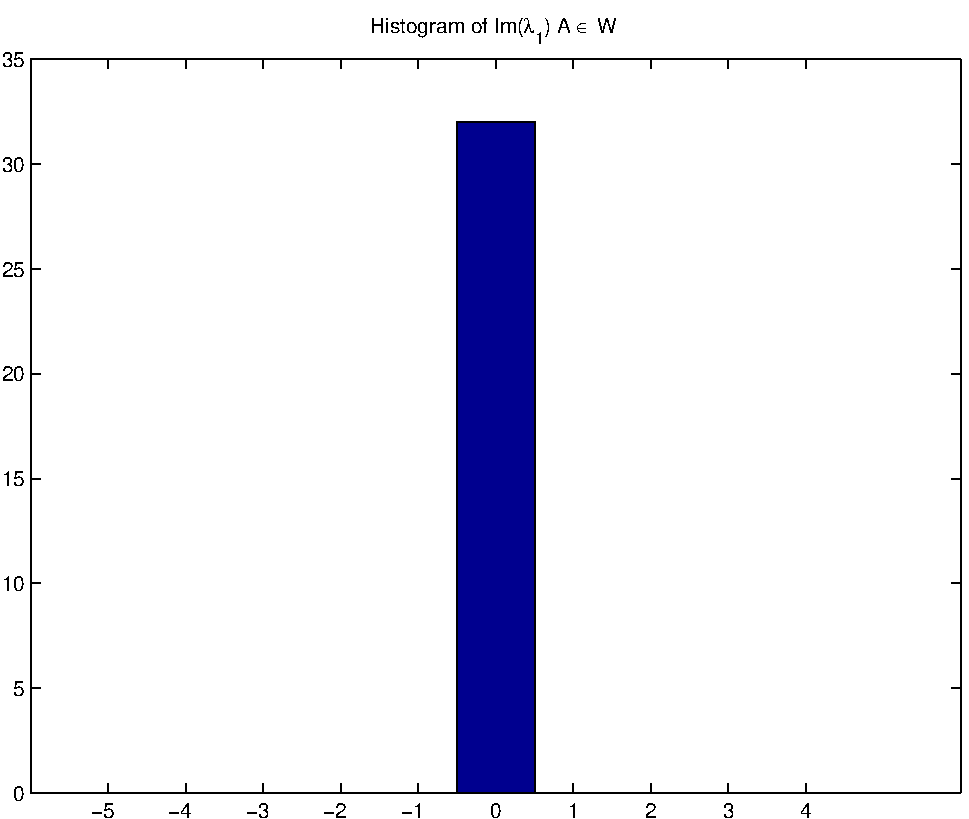
\includegraphics[width=10.0cm,height=10.0cm]{Im_TraceyWidom.pdf}

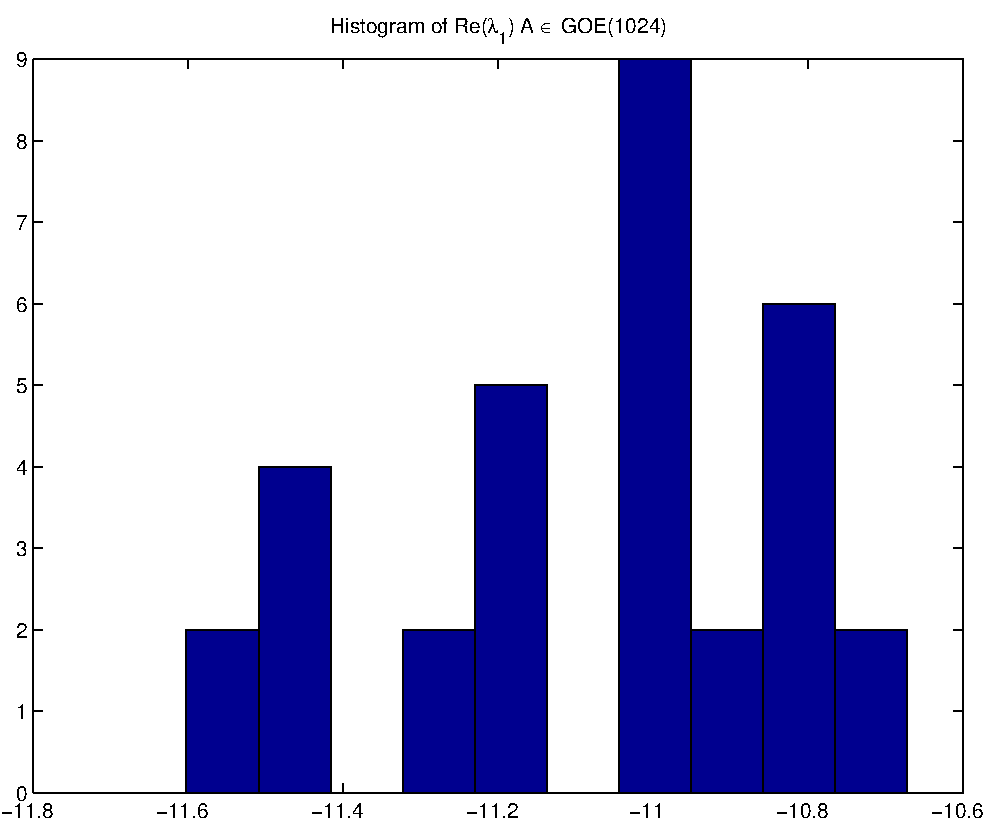
\includegraphics[width=10.0cm,height=10.0cm]{Re_Winger.pdf}

\includegraphics[width=10.0cm,height=10.0cm]{Im_Winger.pdf}

QueryPerformanceCounter  =  +4.791
\subsubsection{Approximate Winger Distribution}
\subsubsection{Verfy Winger Law.}
Let $M_n = [X_{ij} ]$ a symmetric n x n matrix with Random entries such that $X_{i,j} = X_{j,i}$, 		  and $X_{i,j}$ are iid $orall i < j,$ and $Xjj$ are iid $orall j  :  ; E[X^2_{ij} ] = 1, & E[X_{ij}] = 0$ 		  and that all moments exists for each of the entries.  		  The eigenvector of this random matrix; $ lambda_1 leq ... leq lambda_n$ depends continuously on $Mn$.
Dimension $n = +512$

\includegraphics[width=10.0cm,height=10.0cm]{Re_lambda_n.pdf}

\includegraphics[width=10.0cm,height=10.0cm]{Im_lambda_n.pdf}

QueryPerformanceCounter  =  +2.538
\subsubsection{Matrix Exponential }
$SPD Matrix = \left(
\begin{array}{
cccccccc}
+10.539 & -0.499 & -0.010 & +0.368 & +0.465 & -0.492 & -0.126 & +0.437 \\
-0.499 & +7.286 & +0.365 & -0.481 & -0.337 & -0.466 & +0.279 & +0.056 \\
-0.010 & +0.365 & +6.705 & -0.205 & +0.467 & +0.131 & +0.077 & -0.089 \\
+0.368 & -0.481 & -0.205 & +6.496 & -0.402 & -0.209 & +0.043 & -0.041 \\
+0.465 & -0.337 & +0.467 & -0.402 & +4.578 & +0.272 & +0.289 & -0.285 \\
-0.492 & -0.466 & +0.131 & -0.209 & +0.272 & +8.181 & +0.343 & -0.244 \\
-0.126 & +0.279 & +0.077 & +0.043 & +0.289 & +0.343 & +5.938 & -0.212 \\
+0.437 & +0.056 & -0.089 & -0.041 & -0.285 & -0.244 & -0.212 & +9.691 \\
\end{array}
\right)$ \newline 

$SPD Eigs = \left(
\begin{array}{
cccccccc}
(+10.93611,+0.00000) & (+9.60778,+0.00000) & (+4.23666,+0.00000) & (+8.36911,+0.00000) & (+7.56229,+0.00000) & (+5.82791,+0.00000) & (+6.54198,+0.00000) & (+6.33139,+0.00000) \\
\end{array}
\right)$ \newline 

$exp(SPD) = \left(
\begin{array}{
cccccccc}
+47863.969 & -6460.093 & -1078.770 & +4706.958 & +2535.224 & -8475.398 & -2406.368 & +12977.552 \\
-6460.093 & +2780.574 & +516.920 & -1069.918 & -548.083 & -109.707 & +386.466 & -807.216 \\
-1078.770 & +516.920 & +1015.281 & -385.755 & +176.069 & +458.541 & +212.284 & -859.022 \\
+4706.958 & -1069.918 & -385.755 & +1267.210 & +111.181 & -1018.272 & -287.809 & +1036.628 \\
+2535.224 & -548.083 & +176.069 & +111.181 & +413.265 & +135.193 & +45.490 & -502.411 \\
-8475.398 & -109.707 & +458.541 & -1018.272 & +135.193 & +5613.026 & +968.003 & -4270.737 \\
-2406.368 & +386.466 & +212.284 & -287.809 & +45.490 & +968.003 & +632.432 & -1645.725 \\
+12977.552 & -807.216 & -859.022 & +1036.628 & -502.411 & -4270.737 & -1645.725 & +19362.944 \\
\end{array}
\right)$ \newline 

$exp(SPD) eigs = \left(
\begin{array}{
cccccccc}
(+56168.17045,+0.00000) & (+14880.07985,+0.00000) & (+4311.77579,+0.00000) & (+1924.25027,+0.00000) & (+69.17669,+0.00000) & (+339.64809,+0.00000) & (+693.66208,+0.00000) & (+561.93669,+0.00000) \\
\end{array}
\right)$ \newline 

$log(exp(SPD) eigs)  = \left(
\begin{array}{
cccccccc}
(+10.93611,+0.00000) & (+9.60778,+0.00000) & (+8.36911,+0.00000) & (+7.56229,+0.00000) & (+4.23666,+0.00000) & (+5.82791,+0.00000) & (+6.54198,+0.00000) & (+6.33139,+0.00000) \\
\end{array}
\right)$ \newline 

$exp(Id) = \left(
\begin{array}{
cccccccc}
+2.718 & +0.000 & +0.000 & +0.000 & +0.000 & +0.000 & +0.000 & +0.000 \\
+0.000 & +2.718 & +0.000 & +0.000 & +0.000 & +0.000 & +0.000 & +0.000 \\
+0.000 & +0.000 & +2.718 & +0.000 & +0.000 & +0.000 & +0.000 & +0.000 \\
+0.000 & +0.000 & +0.000 & +2.718 & +0.000 & +0.000 & +0.000 & +0.000 \\
+0.000 & +0.000 & +0.000 & +0.000 & +2.718 & +0.000 & +0.000 & +0.000 \\
+0.000 & +0.000 & +0.000 & +0.000 & +0.000 & +2.718 & +0.000 & +0.000 \\
+0.000 & +0.000 & +0.000 & +0.000 & +0.000 & +0.000 & +2.718 & +0.000 \\
+0.000 & +0.000 & +0.000 & +0.000 & +0.000 & +0.000 & +0.000 & +2.718 \\
\end{array}
\right)$ \newline 

$exp(Id) eigs = \left(
\begin{array}{
cccccccc}
(+2.71828,+0.00000) & (+2.71828,+0.00000) & (+2.71828,+0.00000) & (+2.71828,+0.00000) & (+2.71828,+0.00000) & (+2.71828,+0.00000) & (+2.71828,+0.00000) & (+2.71828,+0.00000) \\
\end{array}
\right)$ \newline 

$log(exp(Id) eigs)  = \left(
\begin{array}{
cccccccc}
(+1.00000,+0.00000) & (+1.00000,+0.00000) & (+1.00000,+0.00000) & (+1.00000,+0.00000) & (+1.00000,+0.00000) & (+1.00000,+0.00000) & (+1.00000,+0.00000) & (+1.00000,+0.00000) \\
\end{array}
\right)$ \newline 

For $n  \in  \dblz [16,128)$ we calculate  $|( SPD(n) Eigs - log(exp(SPD(n)) eigs)|_{l^2}$

$|( SPD(n) Eigs - log(exp(SPD(n)) eigs)|_{l^2} = \left(
\begin{array}{
cccccccccccccccccccccccccccccccccccccccccccccccccccccccccccccccccccccccccccccccccccccccccccccccccccccccccccccccc}
(+5.36543,+0.00000) & (+5.36543,+0.00000) & (+5.36543,+0.00000) & (+5.36543,+0.00000) & (+5.36543,+0.00000) & (+5.36543,+0.00000) & (+5.36543,+0.00000) & (+5.36543,+0.00000) & (+5.36543,+0.00000) & (+5.36543,+0.00000) & (+5.36543,+0.00000) & (+5.36543,+0.00000) & (+5.36543,+0.00000) & (+5.36543,+0.00000) & (+5.36543,+0.00000) & (+5.36543,+0.00000) & (+5.36543,+0.00000) & (+5.36543,+0.00000) & (+5.36543,+0.00000) & (+5.36543,+0.00000) & (+5.36543,+0.00000) & (+5.36543,+0.00000) & (+5.36543,+0.00000) & (+5.36543,+0.00000) & (+5.36543,+0.00000) & (+5.36543,+0.00000) & (+5.36543,+0.00000) & (+5.36543,+0.00000) & (+5.36543,+0.00000) & (+5.36543,+0.00000) & (+5.36543,+0.00000) & (+5.36543,+0.00000) & (+5.36543,+0.00000) & (+5.36543,+0.00000) & (+5.36543,+0.00000) & (+5.36543,+0.00000) & (+5.36543,+0.00000) & (+5.36543,+0.00000) & (+5.36543,+0.00000) & (+5.36543,+0.00000) & (+5.36543,+0.00000) & (+5.36543,+0.00000) & (+5.36543,+0.00000) & (+5.36543,+0.00000) & (+5.36543,+0.00000) & (+5.36543,+0.00000) & (+5.36543,+0.00000) & (+5.36543,+0.00000) & (-2.44429,+0.00000) & (-2.23416,+0.00000) & (-2.12272,+0.00000) & (-1.68408,+0.00000) & (-1.46701,+0.00000) & (-1.42424,+0.00000) & (-1.19344,+0.00000) & (-1.00106,+0.00000) & (-0.79899,+0.00000) & (-1.32863,+0.00000) & (-0.03334,+0.00000) & (-0.18953,+0.00000) & (-0.70439,+0.00000) & (-0.53235,+0.00000) & (-0.34237,+0.00000) & (-2.07773,+0.00000) & (-0.59962,+0.00000) & (+11.22991,+0.00000) & (+10.41441,+0.00000) & (+10.46783,+0.00000) & (+9.90149,+0.00000) & (+9.80254,+0.00000) & (+9.43560,+0.00000) & (+9.32668,+0.00000) & (+8.69531,+0.00000) & (+8.60839,+0.00000) & (+8.50649,+0.00000) & (+8.10449,+0.00000) & (+8.00930,+0.00000) & (+7.80818,+0.00000) & (+7.62980,+0.00000) & (+7.49638,+0.00000) & (+7.27792,+0.00000) & (+7.03568,+0.00000) & (+6.93971,+0.00000) & (+6.68496,+0.00000) & (+6.65899,+0.00000) & (+6.18603,+0.00000) & (+6.36871,+0.00000) & (+6.35404,+0.00000) & (+5.89747,+0.00000) & (+5.79944,+0.00000) & (+5.64551,+0.00000) & (+5.48740,+0.00000) & (+5.39983,+0.00000) & (+5.21111,+0.00000) & (+5.10213,+0.00000) & (+5.05172,+0.00000) & (+4.79593,+0.00000) & (+4.74556,+0.00000) & (+4.57093,+0.00000) & (+4.35876,+0.00000) & (+3.88183,+0.00000) & (+4.00029,+0.00000) & (+3.64260,+0.00000) & (+3.45729,+0.00000) & (+3.28400,+0.00000) & (+3.19484,+0.00000) & (+3.07091,+0.00000) & (+2.94105,+0.00000) & (+2.86247,+0.00000) & (+2.58917,+0.00000) & (+2.40251,+0.00000) & (+2.34452,+0.00000) \\
\end{array}
\right)$ \newline 

QueryPerformanceCounter  =  +0.00978
The sample size generated for this run is 100000.

\newpage
uniform \begin{tabular}{|c|c|c|c|}  mean & variance & skewness & kurtosis \\  \hline
$\mu_1 = +0.50030$ & $\mu_2 = +0.08353$ & $\mu_3 = +0.00339$ & $\mu_4 =+1.80113$ \\
\end{tabular}

\includegraphics[width=5cm,height=5cm]{uniform.pdf}

cauchy \begin{tabular}{|c|c|c|c|}  mean & variance & skewness & kurtosis \\  \hline
$\mu_1 = +0.44288$ & $\mu_2 = +0.05341$ & $\mu_3 = +0.63935$ & $\mu_4 =+3.28094$ \\
\end{tabular}

\includegraphics[width=5cm,height=5cm]{cauchy.pdf}

exponential \begin{tabular}{|c|c|c|c|}  mean & variance & skewness & kurtosis \\  \hline
$\mu_1 = +1.99647$ & $\mu_2 = +3.99339$ & $\mu_3 = +2.03097$ & $\mu_4 =+9.30842$ \\
\end{tabular}

\includegraphics[width=5cm,height=5cm]{exponential.pdf}

\newpage
gamma \begin{tabular}{|c|c|c|c|}  mean & variance & skewness & kurtosis \\  \hline
$\mu_1 = +1.89981$ & $\mu_2 = +1.91148$ & $\mu_3 = +1.47441$ & $\mu_4 =+6.41265$ \\
\end{tabular}

\includegraphics[width=5cm,height=5cm]{gamma.pdf}

GIG \begin{tabular}{|c|c|c|c|}  mean & variance & skewness & kurtosis \\  \hline
$\mu_1 = +0.80533$ & $\mu_2 = +10.87636$ & $\mu_3 = +15.18764$ & $\mu_4 =+311.57355$ \\
\end{tabular}

\includegraphics[width=5cm,height=5cm]{GIG.pdf}

normal-box-muller \begin{tabular}{|c|c|c|c|}  mean & variance & skewness & kurtosis \\  \hline
$\mu_1 = +0.00294$ & $\mu_2 = +0.99767$ & $\mu_3 = +0.00740$ & $\mu_4 =+2.98667$ \\
\end{tabular}

\includegraphics[width=5cm,height=5cm]{normal-box-muller.pdf}

\newpage
normal-inverse-approximation \begin{tabular}{|c|c|c|c|}  mean & variance & skewness & kurtosis \\  \hline
$\mu_1 = +0.00230$ & $\mu_2 = +1.00486$ & $\mu_3 = +0.01163$ & $\mu_4 =+2.99254$ \\
\end{tabular}

\includegraphics[width=5cm,height=5cm]{normal-inverse-approximation.pdf}

pareto \begin{tabular}{|c|c|c|c|}  mean & variance & skewness & kurtosis \\  \hline
$\mu_1 = +3184578.26493$ & $\mu_2 = +888468246174112900.00000$ & $\mu_3 = +315.36997$ & $\mu_4 =+99629.09819$ \\
\end{tabular}

\includegraphics[width=5cm,height=5cm]{pareto.pdf}

poisson \begin{tabular}{|c|c|c|c|}  mean & variance & skewness & kurtosis \\  \hline
$\mu_1 = +1.10742$ & $\mu_2 = +0.13228$ & $\mu_3 = +3.87626$ & $\mu_4 =+20.57559$ \\
\end{tabular}

\includegraphics[width=5cm,height=5cm]{poisson.pdf}

\newpage
beta \begin{tabular}{|c|c|c|c|}  mean & variance & skewness & kurtosis \\  \hline
$\mu_1 = +0.33169$ & $\mu_2 = +0.12640$ & $\mu_3 = +0.68838$ & $\mu_4 =+1.92228$ \\
\end{tabular}

\includegraphics[width=5cm,height=5cm]{beta.pdf}

QueryPerformanceCounter  =  +10.69541
\subsubsection{Multiclass Support Vector Machine }
\begin{itemize}
\item Number or training points = 1024
\item Feature dimension = 3
\item Number or classes = 3
\end{itemize}
{The mean vectors of the 3 classes}

$\mu_1 = \left(
\begin{array}{
ccc}
+1.90000 & +0.10000 & +0.10000 \\
\end{array}
\right)$ \newline 

$\mu_2 = \left(
\begin{array}{
ccc}
+0.10000 & +1.90000 & +0.10000 \\
\end{array}
\right)$ \newline 

$\mu_3 = \left(
\begin{array}{
ccc}
+0.00000 & +0.00000 & +1.90000 \\
\end{array}
\right)$ \newline 

A random SPD covairance matrix is generated for each of the classes.\newline

$\rho_1 = \left(
\begin{array}{
ccc}
+3.695 & -0.493 & +0.034 \\
-0.493 & +4.274 & -0.222 \\
+0.034 & -0.222 & +3.709 \\
\end{array}
\right)$ \newline 

$\rho_2 = \left(
\begin{array}{
ccc}
+1.743 & +0.102 & -0.369 \\
+0.102 & +3.495 & -0.053 \\
-0.369 & -0.053 & +3.080 \\
\end{array}
\right)$ \newline 

$\rho_3 = \left(
\begin{array}{
ccc}
+2.926 & -0.175 & +0.045 \\
-0.175 & +1.789 & -0.411 \\
+0.045 & -0.411 & +3.866 \\
\end{array}
\right)$ \newline 

Verify $L_1$ condition number of covariance. The diagonal entries of the matrix have the form $(0.5 + U(0,1) )*dim(Dom(Cov))$
The lower-diagonal entries take the form $U(0,1) - 0.5$. 
The $L_1$ condition numbers are :
\begin{itemize}
\item +1.533
\item +2.466
\item +2.899
\end{itemize}
\includegraphics[width=10.0cm,height=10.0cm]{rv1_corr.pdf}

\includegraphics[width=10.0cm,height=10.0cm]{rv2_corr.pdf}

\includegraphics[width=10.0cm,height=10.0cm]{rv3_corr.pdf}

\includegraphics[width=10.0cm,height=10.0cm]{trainingPoints.pdf}

These are the SVM parameters - the RBF kernel is used\begin{itemize}
\item allOutlierFraction=0.05
\item mixingCoeff=0.3
\item smoThresh=1.0/10000.0
\item sigma=1
\end{itemize}
\includegraphics[width=10.0cm,height=10.0cm]{testPoints.pdf}

The marginal sample moments (mean var skew kurtosis) for training points.\newline
\begin{tabular}{ c |  c  c  c  c}
Feature & $\mu_1$ & $\mu_2$ & $\mu_3$ & $\mu_4$ \\
0 & +0.671 & +1.313 & +0.434& +2.521 \\
\hline
1 & +0.703 & +1.311 & +0.413& +2.501 \\
\hline
2 & +0.701 & +1.417 & +0.347& +2.604 \\
\hline
\end{tabular}
\newline
The marginal sample moments (mean var skew kurtosis) for test points.\newline
\begin{tabular}{ c | c  c  c  c}
Feature & $\mu_1$ & $\mu_2$ & $\mu_3$ & $\mu_4$ \\
0 & +0.677 & +1.240 & +0.566& +2.706\\
\hline
1 & +0.664 & +1.313 & +0.428& +2.526\\
\hline
2 & +0.724 & +1.329 & +0.358& +2.539\\
\hline
\end{tabular}\newline
\includegraphics[width=10.0cm,height=10.0cm]{classDiffs.pdf}

The error rate for this run is +0.229\newline
QueryPerformanceCounter  =  +6.280
\subsubsection{Semidefinite Programming SDPA}
QueryPerformanceCounter  =  +0.005
\end{document}
